%% Dokumentenklasse (Koma Script) -----------------------------------------
\documentclass[%
   %draft,     % Entwurfsstadium
   final,      % fertiges Dokument
	 % --- Paper Settings ---
   paper=a4,% [Todo: add alternatives]
   paper=portrait, % landscape
   pagesize=auto, % driver
   % --- Base Font Size ---
   fontsize=11.5pt,%
	 % --- Koma Script Version ---
   version=last, %
 ]{scrreprt} % Classes: scrartcl, scrreprt, scrbook


% Encoding der Dateien (sonst funktionieren Umlaute nicht)
% Fuer Linux -> utf8
% Fuer Windows, alte Linux Distributionen -> latin1

% Empfohlen latin1, da einige Pakete mit utf8 Zeichen nicht
% funktionieren, z.B: listings, soul.
\usepackage[latin1]{inputenc}
%\usepackage[ansinew]{inputenc}
%\usepackage[utf8]{inputenc}
%\usepackage{ucs}
%\usepackage[utf8x]{inputenc}

%%% Preambel
%%% === Textbody ==============================================================
\KOMAoptions{%
   DIV=11,% (Size of Text Body, higher values = greater textbody)
   % DIV=calc % (also areaset/classic/current/default/last) 
   % -> after setting of spacing necessary!   
   BCOR=5mm% (Bindekorrektur)
}%
%%% === Headings ==============================================================
\KOMAoptions{%
   %%%% headings
	% headings=small,  % Small Font Size, thin spacing above and below
    headings=normal, % Medium Font Size, medium spacing above and below
   %headings=big, % Big Font Size, large spacing above and below
   %
   headings=noappendixprefix, % chapter in appendix as in body text
	headings=nochapterprefix,  % no prefix at chapters
   % headings=appendixprefix,   % inverse of 'noappendixprefix'
   % headings=chapterprefix,    % inverse of 'nochapterprefix'
   % headings=openany,   % Chapters start at any side
   % headings=openleft,  % Chapters start at left side
   %headings=openright, % Chapters start at right side      
   %%% Add/Dont/Auto Dot behind section numbers 
   %%% (see DUDEN as reference)
   % numbers=autoenddot
   % numbers=enddot
   numbers=noenddot
   % secnumdepth=3 % depth of sections numbering (???)
}%
\setcounter{secnumdepth}{3}
%%% === Page Layout ===========================================================
\KOMAoptions{% (most options are for package typearea)
   % twoside=true, % two side layout (alternating margins, standard in books)
    twoside=false, % single side layout 
   % twoside=semi,  % two side layout (non alternating margins!)
   %
   twocolumn=false, % (true)
   %
   headinclude=false,%
   footinclude=false,%
   mpinclude=false,%      
   %
   headlines=2.1,%
	% headheight=2em,%
   headsepline=true,%
   footsepline=false%,%
   %cleardoublepage=empty %plain, headings
}%
%%% === Paragraph Separation ==================================================
\KOMAoptions{%
	% parskip=relative, % change indentation according to fontsize (recommanded)
   parskip=absolute, % do not change indentation according to fontsize
   parskip=false    % indentation of 1em
   % parskip=true   % parksip of 1 line - with free space in last line of 1em
   % parskip=full-  % parksip of 1 line - no adjustment
   % parskip=full+  % parksip of 1 line - with free space in last line of 1/4
   % parskip=full*  % parksip of 1 line - with free space in last line of 1/3
   % parskip=half   % parksip of 1/2 line - with free space in last line of 1em
   % parskip=half-  % parksip of 1/2 line - no adjustment
   % parskip=half+  % parksip of 1/2 line - with free space in last line of 1/3
   % parskip=half*  % parksip of 1/2 line - with free space in last line of 1em
}%
%%% === Table of Contents =====================================================
\setcounter{tocdepth}{3} % Depth of TOC Display
\KOMAoptions{%
   %%% Setting of 'Style' and 'Content' of TOC
   % toc=left, %
   toc=indented,%
   %
   toc=bib,
   % toc=nobib,
   % toc=bibnumbered,
   %
	% toc=index,%
   toc=noindex,
   %
   % toc=listof,
   toc=nolistof
   % toc=listofnumbered,
   %   
}%  
%%% === Lists of figures, tables etc. =========================================
\KOMAoptions{%
   %%% Setting of 'Style' and 'Content' of Lists 
   %%% (figures, tables etc)
	% --- General List Style ---
   listof=left, % tabular styles
   listof=indented, % hierarchical style
   % --- chapter highlighting ---
   % listof=chapterentry, % ??? Chapter starts are marked in figure/table
   % listof=chaptergapline, % New chapter starts are marked by a gap 
      		  			   	 % of a single line
	listof=chaptergapsmall, % New chapter starts are marked by a gap 
   	    					   % of a smallsingle line
   % listof=nochaptergap, % No Gap between chapters
   %
   % listof=leveldown, % lists are moved one level down ???
   % --- Appearance of Lists in TOC
   % listof=notoc, % Lists are not part of the TOC
   listof=totoc % add Lists to TOC without number
   % listof=totocnumbered, % add Lists to TOC with number
}%  
%%% === Bibliography ==========================================================
%% Setting of 'Style' and 'Content' of Bibliography
\KOMAoptions{%
	% bibliography=oldstyle,%
   bibliography=openstyle,%
   % bibliography=nottotoc, % Bibliography is not part of the TOC
   % bibliography=totocnumbered, % add Bibliography to TOC with number
   bibliography=totoc % add Bibliography to TOC without number
}%
%%% === Index =================================================================
%% Setting of 'Style' and 'Content' of Index in TOC
\KOMAoptions{%
   %index=nottotoc % index is not part of the TOC
	 %index=totoc % add index to TOC without number
}%
%%% === Titlepage =============================================================
\KOMAoptions{%
   titlepage=true %
   %titlepage=false %
}%
%%% === Miscellaneous =========================================================
\KOMAoptions{% 	
   footnotes=multiple% nomultiple
   %open=any,%
   %open=left,%
   %open=right,%
   %chapterprefix=false,%
   %appendixprefix=false,%
   %chapteratlists=10pt,% entry
}%
% ------------------------------------------------------------------------
% LaTeX - Preambel  ******************************************************
% ------------------------------------------------------------------------
% von: Matthias Pospiech
% ========================================================================

% Strukturierung dieser Praeambel:
%    1.  Pakete die vor anderen geladen werden m�ssen
%        (calc, babel, xcolor, graphicx, amsmath, pst-pdf, ragged2e, ...)
%    2.  Schriften
%    3.  Mathematik (mathtools, fixmath, onlyamsmath, braket,
%        cancel, empheq, exscale, icomma, ...)
%    4.  Tabellen (booktabs, multirow, dcolumn, tabularx, ltxtable, supertabular)
%    5.  Text
%        5.1 Auszeichnungen (ulem, soul, url)
%        5.2 Fussnoten (footmisc)
%        5.3 Verweise (varioref)
%        5.4 Listen (enumitem, paralist, declist)
%    6.  Zitieren (csquotes, jurabib, natbib)
%    7.  PDF (microtype, hyperref, backref, hypcap, pdfpages
%    8.  Graphiken (float, flafter, placeins, subfig, wrapfig,
%        floatflt, picins, psfrag, sidecap, pict2e, curve2e)
%    9.  Sonstiges (makeidx, isodate, numprint, nomencl, acronym)
%    10. Verbatim (upquote, verbatim, fancyvrb, listings, examplep)
%    11. Wissenschaft (units)
%    12. Fancy Stuff
%    13. Layout
%       13.1.  Diverse Pakete und Einstellungen (multicol, ellipsis)
%       13.2.  Zeilenabstand (setspace)
%       13.3.  Seitenlayout (typearea, geometry)
%       13.4.  Farben
%       13.5.  Aussehen der URLS
%       13.6.  Kopf und Fusszeilen (scrpage2)
%       13.7.  Fussnoten
%       13.8.  Schriften (Sections )
%       13.9.  UeberSchriften (Chapter und Sections) (titlesec, indentfirst)
%       13.10. Captions (Schrift, Aussehen)
%              (caption, subfig, capt-of, mcaption, tocloft, multitoc, minitoc)
%    14.  Auszufuehrende Befehle


% ~~~~~~~~~~~~~~~~~~~~~~~~~~~~~~~~~~~~~~~~~~~~~~~~~~~~~~~~~~~~~~~~~~~~~~~~
% Einige Pakete muessen unbedingt vor allen anderen geladen werden
% ~~~~~~~~~~~~~~~~~~~~~~~~~~~~~~~~~~~~~~~~~~~~~~~~~~~~~~~~~~~~~~~~~~~~~~~~

%%% Packages for LaTeX - programming
%
% Define commands that don't eat spaces.
\usepackage{xspace}
% IfThenElse
\usepackage{ifthen}
%%% Doc: ftp://tug.ctan.org/pub/tex-archive/macros/latex/contrib/oberdiek/ifpdf.sty
% command for testing for pdf-creation
\usepackage{ifpdf} %\ifpdf \else \fi

%%% Internal Commands: ----------------------------------------------
\makeatletter
%
\providecommand{\IfPackageLoaded}[2]{\@ifpackageloaded{#1}{#2}{}}
\providecommand{\IfPackageNotLoaded}[2]{\@ifpackageloaded{#1}{}{#2}}
\providecommand{\IfElsePackageLoaded}[3]{\@ifpackageloaded{#1}{#2}{#3}}
%
\newboolean{chapteravailable}%
\setboolean{chapteravailable}{false}%

\ifcsname chapter\endcsname
  \setboolean{chapteravailable}{true}%
\else
  \setboolean{chapteravailable}{false}%
\fi


\providecommand{\IfChapterDefined}[1]{\ifthenelse{\boolean{chapteravailable}}{#1}{}}%
\providecommand{\IfElseChapterDefined}[2]{\ifthenelse{\boolean{chapteravailable}}{#1}{#2}}%

\providecommand{\IfDefined}[2]{%
\ifcsname #1\endcsname
   #2 %
\else
     % do nothing
\fi
}

\providecommand{\IfElseDefined}[3]{%
\ifcsname #1\endcsname
   #2 %
\else
   #3 %
\fi
}

\providecommand{\IfElseUnDefined}[3]{%
\ifcsname #1\endcsname
   #3 %
\else
   #2 %
\fi
}


%
% Check for 'draft' mode - commands.
\newcommand{\IfNotDraft}[1]{\ifx\@draft\@undefined #1 \fi}
\newcommand{\IfNotDraftElse}[2]{\ifx\@draft\@undefined #1 \else #2 \fi}
\newcommand{\IfDraft}[1]{\ifx\@draft\@undefined \else #1 \fi}
%

% Definde frontmatter, mainmatter and backmatter if not defined
\@ifundefined{frontmatter}{%
   \newcommand{\frontmatter}{%
      %In Roemischen Buchstaben nummerieren (i, ii, iii)
      \pagenumbering{roman}
   }
}{}
\@ifundefined{mainmatter}{%
   % scrpage2 benoetigt den folgenden switch
   % wenn \mainmatter definiert ist.
   \newif\if@mainmatter\@mainmattertrue
   \newcommand{\mainmatter}{%
      % -- Seitennummerierung auf Arabische Zahlen zuruecksetzen (1,2,3)
      \pagenumbering{arabic}%
      \setcounter{page}{1}%
   }
}{}
\@ifundefined{backmatter}{%
   \newcommand{\backmatter}{
      %In Roemischen Buchstaben nummerieren (i, ii, iii)
      \pagenumbering{roman}
   }
}{}

% Pakete speichern die spaeter geladen werden sollen
\newcommand{\LoadPackagesNow}{}
\newcommand{\LoadPackageLater}[1]{%
   \g@addto@macro{\LoadPackagesNow}{%
      \usepackage{#1}%
   }%
}



\makeatother
%%% ----------------------------------------------------------------
%
%%% Doc: www.cs.brown.edu/system/software/latex/doc/calc.pdf
% Calculation with LaTeX
\usepackage{calc}

%%% Doc: ftp://tug.ctan.org/pub/tex-archive/macros/latex/required/babel/babel.pdf
% Languagesetting
\usepackage[
%	german,
%	ngerman,
	english,
%	french,
]{babel}

%%% Doc: ftp://tug.ctan.org/pub/tex-archive/macros/latex/contrib/xcolor/xcolor.pdf
% Farben
% Incompatible: Do not load when using pstricks !
\usepackage[
	table % Load for using rowcolors command in tables
]{xcolor}


%%% Doc: ftp://tug.ctan.org/pub/tex-archive/macros/latex/required/graphics/grfguide.pdf
% Bilder
\usepackage[%
	%final,
	%draft % do not include images (faster)
]{graphicx}

%%% Doc: ftp://tug.ctan.org/pub/tex-archive/macros/latex/contrib/oberdiek/epstopdf.pdf
%% If an eps image is detected, epstopdf is automatically called to convert it to pdf format.
%% Requires: graphicx loaded
\usepackage{epstopdf}


%%% Doc: ftp://tug.ctan.org/pub/tex-archive/macros/latex/required/amslatex/math/amsldoc.pdf
% Amsmath - Mathematik Basispaket
%
% fuer pst-pdf displaymath Modus vor pst-pdf benoetigt.
\usepackage[
   centertags, % (default) center tags vertically
   %tbtags,    % 'Top-or-bottom tags': For a split equation, place equation numbers level
               % with the last (resp. first) line, if numbers are on the right (resp. left).
   sumlimits,  %(default) Place the subscripts and superscripts of summation
               % symbols above and below
   %nosumlimits, % Always place the subscripts and superscripts of summation-type
               % symbols to the side, even in displayed equations.
   intlimits,  % Like sumlimits, but for integral symbols.
   %nointlimits, % (default) Opposite of intlimits.
   namelimits, % (default) Like sumlimits, but for certain 'operator names' such as
               % det, inf, lim, max, min, that traditionally have subscripts placed underneath
               % when they occur in a displayed equation.
   %nonamelimits, % Opposite of namelimits.
   %leqno,     % Place equation numbers on the left.
   %reqno,     % Place equation numbers on the right.
   fleqn,     % Position equations at a fixed indent from the left margin
   			  % rather than centered in the text column.
]{amsmath} %
% eqnarray nicht zusammen mit amsmath benutzen, siehe l2tabu.pdf f�r
% Hintergruende.

%%% Doc: http://www.ctan.org/tex-archive/macros/latex/contrib/pst-pdf/pst-pdf-DE.pdf
% Used to automatically integrate eps graphics in an pdf document using pdflatex.
% Requires ps4pdf macro !!!
% Download macro from http://www.ctan.org/tex-archive/macros/latex/contrib/pst-pdf/scripts/
%
%\usepackage[%
%   %active,       % Aktiviert den Extraktionsmodus (DVI-Ausgabe). Die explizite Angabe ist
%                  % normalerweise unn�tig (Standard im LATEX-Modus).
%   %inactive,     % Das Paket wird deaktiviert, Zu�tzlich werden die Pakete pstricks und
%                  % graphicx geladen
%   nopstricks,    % Das Paket pstricks wird nicht geladen.
%   %draft,        % Im pdfLATEX-Modus werden aus der Containerdatei eingef�gte Grafiken nur
%                  % als Rahmen dargestellt.
%   %final,        % Im pdfLATEX-Modus werden aus der Containerdatei eingef�gte Grafiken
%                  % vollst�ndig dargestellt (Standard).
%   %tightpage,    % Die Abmessung Grafiken in der Containerdatei entsprechen denen der
%                  % zugeh�rigen TEX-Boxen (Standard).
%   %notightpage,  % die Grafiken in der Containerdatei nehmen
%                  % mindestens die Gr��e des gesamten Blattes einnehmen.
%   %displaymath,  % Es werden zus�tzlich die mathematischen Umgebungen displaymath,
%                  % eqnarray und $$ extrahiert und im pdf-Modus als Grafik eingef�gt.
%]{pst-pdf}
%
% Notwendiger Bugfix f�r natbib Paket bei Benutzung von pst-pdf (Version <= v1.1o)
\IfPackageLoaded{pst-pdf}{
   \providecommand\makeindex{}
   \providecommand\makeglossary{}
}{}


%% Doc: ftp://tug.ctan.org/pub/tex-archive/graphics/pstricks/README
% load before graphicx
% \usepackage{pstricks}
% \usepackage{pst-plot, pst-node, pst-coil, pst-eps}

% This package implements a workaround for the LaTeX bug that marginpars
% sometimes appear on the wrong margin.
% \usepackage{mparhack}
% in some case this causes an error in the index together with package pdfpages
% the reason is unkown. Therefore I recommend to use the margins of marginnote

%% Doc: ftp://tug.ctan.org/pub/tex-archive/macros/latex/contrib/marginnote/marginnote.pdf
% Summary description: marginnote allows margin note, where \marginpar fails
\usepackage{marginnote}


%% Doc: (inside relsize.sty )
%% ftp://tug.ctan.org/pub/tex-archive/macros/latex/contrib/misc/relsize.sty
%  Set the font size relative to the current font size
\usepackage{relsize}

%% Doc: ftp://tug.ctan.org/pub/tex-archive/macros/latex/contrib/ms/ragged2e.pdf
% Besserer Flatternsatz (Linksbuendig, statt Blocksatz)
\usepackage{ragged2e}

% ~~~~~~~~~~~~~~~~~~~~~~~~~~~~~~~~~~~~~~~~~~~~~~~~~~~~~~~~~~~~~~~~~~~~~~~~
% Fonts Fonts Fonts
% ~~~~~~~~~~~~~~~~~~~~~~~~~~~~~~~~~~~~~~~~~~~~~~~~~~~~~~~~~~~~~~~~~~~~~~~~

\usepackage[T1]{fontenc} % T1 Schrift Encoding
\usepackage{textcomp}	 % Zusatzliche Symbole (Text Companion font extension)

%%% Schriften werden in Fonts.tex geladen
% ~~~~~~~~~~~~~~~~~~~~~~~~~~~~~~~~~~~~~~~~~~~~~~~~~~~~~~~~~~~~~~~~~~~~~~~~
% Fonts Fonts Fonts
% ~~~~~~~~~~~~~~~~~~~~~~~~~~~~~~~~~~~~~~~~~~~~~~~~~~~~~~~~~~~~~~~~~~~~~~~~

% Alle Schriften die hier angegeben sind sehen im PDF richtig aus.
% Die LaTeX Standardschrift ist die Latin Modern (lmodern Paket).
% If Latin Modern is not available for your distribution you must install the
% package cm-super instead. Otherwise your fonts will look horrible in the PDF

% DO NOT LOAD ae Package for the font !

%% ==== Zusammengesetzte Schriften  (Sans + Serif) =======================

%% - Latin Modern
\usepackage{lmodern}
%% -------------------
%
%% - Times, Helvetica, Courier (Word Standard...)
%\usepackage{mathptmx}
%\usepackage[scaled=.90]{helvet}
%\usepackage{courier}
%% -------------------
%%
%% - Palantino , Helvetica, Courier
%\usepackage{mathpazo}
%\usepackage[scaled=.95]{helvet}
%\usepackage{courier}
%% -------------------
%
%% - Bera Schriften
%\usepackage{bera}
%% -------------------
%
%% - Charter, Bera Sans
%\usepackage{charter}\linespread{1.05}
%\renewcommand{\sfdefault}{fvs}

%% ===== Serifen =========================================================

%\usepackage{mathpazo}                 %% --- Palantino
%\usepackage{charter}\linespread{1.05} %% --- Charter
%\usepackage{bookman}                  %% --- Bookman (laedt Avant Garde !!)
%\usepackage{newcent}                  %% --- New Century Schoolbook (laedt Avant Garde !!)

%\usepackage[%                         %% --- Fourier
%   upright,     % Math fonts are upright
%   expert,      % Only for EXPERT Fonts!
%   oldstyle,    % Only for EXPERT Fonts!
%   fulloldstyle % Only for EXPERT Fonts!
%]{fourier} %



%% ===== Sans Serif ======================================================

%\usepackage[scaled=.95]{helvet}        %% --- Helvetica
%\usepackage{cmbright}                  %% --- CM-Bright (eigntlich eine Familie)
%\usepackage{tpslifonts}                %% --- tpslifonts % Font for Slides
%\usepackage{avantgar}                  %% --- Avantgarde

%%%% =========== Italics ================

%\usepackage{chancery}                  %% --- Zapf Chancery

%%%% =========== Typewriter =============

%\usepackage{courier}                   %% --- Courier
%\renewcommand{\ttdefault}{cmtl}        %% --- CmBright Typewriter Font
%\usepackage[%                          %% --- Luxi Mono (Typewriter)
%   scaled=0.9
%]{luximono}



%%%% =========== Mathe ================

%% Recommanded to use with fonts: Aldus, Garamond, Melior, Sabon
%\usepackage[                           %% --- EulerVM (MATH)
%   small,       %for smaller Fonts
%  euler-digits % digits in euler fonts style
%]{eulervm}

% \usepackage[
% %   utopia,
% %   garamond,
%    charter
% ]{mathdesign}

%%%% (((( !!! kommerzielle Schriften !!! )))))))))))))))))))))))))))))))))))))))))))))))))))

%% ===== Serifen (kommerzielle Schriften ) ================================

%% --- Adobe Aldus
%\renewcommand{\rmdefault}{pasx}
%\renewcommand{\rmdefault}{pasj} %%oldstyle digits
% math recommended: \usepackage[small]{eulervm}

%% --- Adobe Garamond
%\usepackage[%
%   osf,        % oldstyle digits
%   scaled=1.05 %appropriate in many cases
%]{xagaramon}
% math recommended: \usepackage{eulervm}

%% --- Adobe Stempel Garamond
%\renewcommand{\rmdefault}{pegx}
%\renewcommand{\rmdefault}{pegj} %%oldstyle digits

%% --- Adobe Melior
%\renewcommand{\rmdefault}{pml}
% math recommended: %\usepackage{eulervm}

%% --- Adobe Minion
%\renewcommand{\rmdefault}{pmnx}
%\renewcommand{\rmdefault}{pmnj} %oldstyle digits
% math recommended: \usepackage[small]{eulervm} or \usepackage{mathpmnt} % commercial

%% --- Adobe Sabon
%\renewcommand{\rmdefault}{psbx}
%\renewcommand{\rmdefault}{psbj} %oldstyle digits
% math recommended: \usepackage{eulervm}

%% --- Adobe Times
% math recommended: \usepackage{mathptmx} % load first !
%\renewcommand{\rmdefault}{ptmx}
%\renewcommand{\rmdefault}{ptmj} %oldstyle digits

%% --- Linotype ITC Charter
%\renewcommand{\rmdefault}{lch}

%% --- Linotype Meridien
%\renewcommand{\rmdefault}{lmd}

%%% ===== Sans Serif (kommerzielle Schriften) ============================

%% --- Adobe Frutiger
%\usepackage[
%   scaled=0.90
%]{frutiger}

%% --- Adobe Futura (=Linotype FuturaLT) : Sans Serif
%\usepackage[
%   scaled=0.94  % appropriate in many cases
%]{futura}

%% --- Adobe Gill Sans : Sans Serif
%\usepackage{gillsans}

%% -- Adobe Myriad  : Sans Serif
%\renewcommand{\sfdefault}{pmy}
%\renewcommand{\sfdefault}{pmyc} %% condensed Font

%% --- Syntax : sans serif font
%\usepackage[
%   scaled
%]{asyntax}

%% --- Adobe Optima : Semi Sans Serif
%\usepackage[
%   medium %darker medium weight fonts
%]{optima}

%% --- Linotype ITC Officina Sans
%\renewcommand{\sfdefault}{lo9}





% ~~~~~~~~~~~~~~~~~~~~~~~~~~~~~~~~~~~~~~~~~~~~~~~~~~~~~~~~~~~~~~~~~~~~~~~~
% Math Packages
% ~~~~~~~~~~~~~~~~~~~~~~~~~~~~~~~~~~~~~~~~~~~~~~~~~~~~~~~~~~~~~~~~~~~~~~~~

% *** Mathematik **************************************
%
% amsmath schon vorher geladen da es vor pst-pdf geladen werden muss


%%% Doc: ftp://tug.ctan.org/pub/tex-archive/macros/latex/contrib/mh/doc/mathtools.pdf
% Erweitert amsmath und behebt einige Bugs
\usepackage[fixamsmath,disallowspaces]{mathtools}

%%% Doc: http://www.ctan.org/info?id=fixmath
% LaTeX's default style of typesetting mathematics does not comply
% with the International Standards ISO31-0:1992 to ISO31-13:1992
% which indicate that uppercase Greek letters always be typset
% upright, as opposed to italic (even though they usually
% represent variables) and allow for typsetting of variables in a
% boldface italic style (even though the required fonts are
% available). This package ensures that uppercase Greek be typeset
% in italic style, that upright $\Delta$ and $\Omega$ symbols are
% available through the commands \upDelta and \upOmega; and
% provides a new math alphabet \mathbold for boldface
% italic letters, including Greek.
\usepackage{fixmath}

%%% Doc: ftp://tug.ctan.org/pub/tex-archive/macros/latex/contrib/onlyamsmath/onlyamsmath.dvi
% Warnt bei Benutzung von Befehlen die mit amsmath inkompatibel sind.
\usepackage[
	all,
	warning
]{onlyamsmath}


%------------------------------------------------------

% -- Vektor fett darstellen -----------------
% \let\oldvec\vec
% \def\vec#1{{\boldsymbol{#1}}} %Fetter Vektor
% \newcommand{\ve}{\vec} %
% -------------------------------------------


%%% Doc: ftp://tug.ctan.org/pub/tex-archive/macros/latex/contrib/misc/braket.sty
\usepackage{braket}  % Quantenmechanik Bracket Schreibweise

%%% Doc: ftp://tug.ctan.org/pub/tex-archive/macros/latex/contrib/misc/cancel.sty
\usepackage{cancel}  % Durchstreichen

%%% Doc: ftp://tug.ctan.org/pub/tex-archive/macros/latex/contrib/mh/doc/empheq.pdf
\usepackage{empheq}  % Hervorheben

%%% Doc: ftp://tug.ctan.org/pub/tex-archive/info/math/voss/mathmode/Mathmode.pdf
%\usepackage{exscale} % Skaliert Mathe-Modus Ausgaben in allen Umgebungen richtig.

%%% Doc: ftp://tug.ctan.org/pub/tex-archive/macros/latex/contrib/was/icomma.dtx
% Erlaubt die Benutzung von Kommas im Mathematikmodus
\usepackage{icomma}


%%% Doc: http://www.ctex.org/documents/packages/special/units.pdf
% \usepackage[nice]{nicefrac}

%%% Tauschen von Epsilon und andere:
% \let\ORGvarrho=\varrho
% \let\varrho=\rho
% \let\rho=\ORGvarrho
%
\let\ORGvarepsilon=\varepsilon
\let\varepsilon=\epsilon
\let\epsilon=\ORGvarepsilon
%
% \let\ORGvartheta=\vartheta
% \let\vartheta=\theta
% \let\theta=\ORGvartheta
%
% \let\ORGvarphi=\varphi
% \let\varphi=\phi
% \let\phi=\ORGvarphi

% ~~~~~~~~~~~~~~~~~~~~~~~~~~~~~~~~~~~~~~~~~~~~~~~~~~~~~~~~~~~~~~~~~~~~~~~~
% Symbole
% ~~~~~~~~~~~~~~~~~~~~~~~~~~~~~~~~~~~~~~~~~~~~~~~~~~~~~~~~~~~~~~~~~~~~~~~~
%
%%% General Doc: http://www.ctan.org/tex-archive/info/symbols/comprehensive/symbols-a4.pdf
%
%% Symbole f�r Mathematiksatz
%\usepackage{mathrsfs} %% Schreibschriftbuchstaben f�r den Mathematiksatz (nur Gro�buchstaben)
%\usepackage{dsfont}   %% Double Stroke Fonts
%\usepackage[mathcal]{euscript} %% adds euler mathcal font
%\usepackage{amssymb}
\usepackage[Symbolsmallscale]{upgreek} % upright symbols from euler package [Euler] or Adobe Symbols [Symbol]
\usepackage[upmu]{gensymb}             % Option upmu

%% Allgemeine Symbole
%\usepackage{wasysym}  %% Doc: http://www.ctan.org/tex-archive/macros/latex/contrib/wasysym/wasysym.pdf
%\usepackage{marvosym} %% Symbole aus der marvosym Schrift
%\usepackage{pifont}   %% ZapfDingbats


% ~~~~~~~~~~~~~~~~~~~~~~~~~~~~~~~~~~~~~~~~~~~~~~~~~~~~~~~~~~~~~~~~~~~~~~~~
% Tables (Tabular)
% ~~~~~~~~~~~~~~~~~~~~~~~~~~~~~~~~~~~~~~~~~~~~~~~~~~~~~~~~~~~~~~~~~~~~~~~~

% Basispaket fuer alle Tabellenfunktionen
% -> wird automatisch durch andere Pakete geladen
% \usepackage{array}
%
% bessere Abstaende innerhalb der Tabelle (Layout))
% -------------------------------------------------
%%% Doc: ftp://tug.ctan.org/pub/tex-archive/macros/latex/contrib/booktabs/booktabs.pdf
\usepackage{booktabs}
%
% Farbige Tabellen
% ----------------
% Das Paket colortbl wird inzwischen automatisch durch xcolor geladen
%
% Erweiterte Funktionen innerhalb von Tabellen
% --------------------------------------------
%%% Doc: ftp://tug.ctan.org/pub/tex-archive/macros/latex/contrib/multirow/multirow.sty
\usepackage{multirow} % Mehrfachspalten
%
%%% Doc: Documentation inside dtx Package
\usepackage{dcolumn}  % Ausrichtung an Komma oder Punkt

%%% Neue Tabellen-Umgebungen:
% ---------------------------
% Spalten automatischer Breite:
%%% Doc: Documentation inside dtx Package
% \usepackage{tabularx}
% -> nach hyperref Laden
% -> wird von ltxtable geladen
% \LoadPackageLater{tabularx}


% Tabellen ueber mehere Seiten
% ----------------------------
%%% Doc: ftp://tug.ctan.org/pub/tex-archive/macros/latex/contrib/carlisle/ltxtable.pdf
% \usepackage{ltxtable} % Longtable + tabularx
                        % (multi-page tables) + (auto-sized columns in a fixed width table)
% -> nach hyperref laden
\LoadPackageLater{ltxtable}


%%% Doc: ftp://tug.ctan.org/pub/tex-archive/macros/latex/contrib/supertabular/supertabular.pdf
%\usepackage{supertabular}


% ~~~~~~~~~~~~~~~~~~~~~~~~~~~~~~~~~~~~~~~~~~~~~~~~~~~~~~~~~~~~~~~~~~~~~~~~
% text related packages
% ~~~~~~~~~~~~~~~~~~~~~~~~~~~~~~~~~~~~~~~~~~~~~~~~~~~~~~~~~~~~~~~~~~~~~~~~

%%% Textverzierungen/Auszeichnungen ======================================
%
%%% Doc: ftp://tug.ctan.org/pub/tex-archive/macros/latex/contrib/misc/ulem.sty
\usepackage[normalem]{ulem}      % Zum Unterstreichen
%%% Doc: ftp://tug.ctan.org/pub/tex-archive/macros/latex/contrib/soul/soul.pdf
\usepackage{soul}		            % Unterstreichen, Sperren
%%% Doc: ftp://tug.ctan.org/pub/tex-archive/macros/latex/contrib/misc/url.sty
\usepackage{url} % Setzen von URLs. In Verbindung mit hyperref sind diese auch aktive Links.

%%% Fussnoten/Endnoten ===================================================
%
%%% Doc: ftp://tug.ctan.org/pub/tex-archive/macros/latex/contrib/footmisc/footmisc.pdf
%
\usepackage[
   bottom,      % Footnotes appear always on bottom. This is necessary
                % especially when floats are used
   stable,      % Make footnotes stable in section titles
   perpage,     % Reset on each page
   %para,       % Place footnotes side by side of in one paragraph.
   %side,       % Place footnotes in the margin
   ragged,      % Use RaggedRight
   %norule,     % suppress rule above footnotes
   multiple,    % rearrange multiple footnotes intelligent in the text.
   %symbol,     % use symbols instead of numbers
]{footmisc}

\renewcommand*{\multfootsep}{,\nobreakspace}

\deffootnote%
   [1em]% width of marker
   {1.5em}% indentation (general)
   {1em}% indentation (par)
   {\textsubscript{\thefootnotemark}}%


%% Einruecken der Fussnote einstellen
%\setlength\footnotemargin{10pt}

%--- footnote counter documentweit durchlaufend ------------------------------
\usepackage{chngcntr}
%\counterwithout{footnote}{chapter}
%-----------------------------------------------------------------------------

%%% Doc: ftp://tug.ctan.org/pub/tex-archive/macros/latex/contrib/misc/endnotes.sty
%\usepackage{endnotes}
% From the Documentation:
% To turn all the footnotes in your documents into endnotes, say
%
%     \let\footnote=\endnote
%
%  in your preamble, and then add something like
%
%     \newpage
%     \begingroup
%     \parindent 0pt
%     \parskip 2ex
%     \def\enotesize{\normalsize}
%     \theendnotes
%     \endgroup
%
% as the last thing in your document.  (But \theendnotes all
% by itself will work.)

%%% Verweise =============================================================
%
%%% Doc: Documentation inside dtx File
%\usepackage[ngerman]{varioref} % Intelligente Querverweise
\usepackage[english]{varioref} % Intelligente Querverweise

%%% Listen ===============================================================
%
%
%%% Doc: ftp://tug.ctan.org/pub/tex-archive/macros/latex/contrib/paralist/paralist.pdf
% \usepackage{paralist}
%
%%% Doc: ftp://tug.ctan.org/pub/tex-archive/macros/latex/contrib/enumitem/enumitem.pdf
% Better than 'paralist' and 'enumerate' because it uses a keyvalue interface !
% Do not load together with enumerate.
\IfPackageNotLoaded{enumerate}{
	\usepackage{enumitem}
}
%
%%% Doc: ftp://tug.ctan.org/pub/tex-archive/macros/latex/contrib/ncctools/doc/desclist.pdf
% Improved description environment
%\usepackage{declist}


% ~~~~~~~~~~~~~~~~~~~~~~~~~~~~~~~~~~~~~~~~~~~~~~~~~~~~~~~~~~~~~~~~~~~~~~~~
% Pakete zum Zitieren
% ~~~~~~~~~~~~~~~~~~~~~~~~~~~~~~~~~~~~~~~~~~~~~~~~~~~~~~~~~~~~~~~~~~~~~~~~

% Quotes =================================================================
%% Doc: ftp://tug.ctan.org/pub/tex-archive/macros/latex/contrib/csquotes/csquotes.pdf
% Advanced features for clever quotations
\usepackage[%
   babel,            % the style of all quotation marks will be adapted
                     % to the document language as chosen by 'babel'
   german=quotes,		% Styles of quotes in each language
   english=british,
   french=guillemets
]{csquotes}

% All facilities which take a 'cite' argument will not insert
% it directly. They pass it to an auxiliary command called \mkcitation
% which  may be redefined to format the citation.
\renewcommand*{\mkcitation}[1]{{\,}#1}
\renewcommand*{\mkccitation}[1]{ #1}

\SetBlockThreshold{2} % Anzahl von Zeilen

\newenvironment{myquote}%
	{\begin{quote}\small}%
	{\end{quote}}%
\SetBlockEnvironment{myquote}
%\SetCiteCommand{} % Changes citation command


% Zitate =================================================================
%
% Reference by number
% \makeatletter
% \renewcommand\@biblabel[1]{#1.}
% \makeatother

% -------- Reference by author -------------------------------------------

% Doc: http://www.berger-on.net/jurabib/
% \usepackage{jurabib}
% \jurabibsetup{
%    authorformat={
%       %abbrv,%  First names will be abbreviated
%       %allreversed,% Names will be printed reversed ('first surname' in text and bibliography)
%       %citationreversed,% Names will be printed reversed ('first surname' only in text)
%       and,% Author separation with ',' and ', and' instead of the default slashes
%       %dynamic,% Font of author depends on existence of coauthor
%       %firstnotreversed, %All author names (except the first) will be printed reversed (in text only)
%       %indexed,% All author names are indexed separately (makeidx or index have to be loaded appropriately)
%       %italic,% Author will appear in italics
%       %reducedifibidem,%  Author names are reduced to the surname for subsequent
%       %citations,% (for the ibidem=name options)
%       smallcaps,% Author will appear in small caps
%       year,% Emulates author-year citations
%    },
%    bibformat={
%       %compress,% Reduces the vertical space between the items in the bibliography
%       %ibidem,%  Replaces repeated authors in the bibliography
%       %ibidemalt,% Special format for German law students
%       %nohang,% No hanging indent for bibliography
%       numbered,% Numbered items in bibliography
%       %raggedright,% Flushleft for bibliography
%       %tabular,% Tabular-like bibliography format
%    },
%    titleformat={
%       all,% Prints out all titles, doesn't care about multiple works
%       %colonsep,% Separation between author and title with colon
%       comma,% Separation between author and title with comma
%       italic,% Title will appear in italics
%    },
%    %biblikecite=true,% Formatting of bibliography follows formatting of citations (as far as possible)
%    %coauthorformat={
%    %  normal,% No special format for coauthors
%    %  %italic,% Coauthor will appear in italics
%    %},
%    %colastsep=divis,% Coauthor after author, separation with divis, Standard is a slash
%    %cofirstsep={
%    %% in,% Author after coauthor, separation with 'in'
%    %  comma,% Author after coauthor, separation with comma
%    %},
%    commabeforerest,  % Nach allen Angaben und vor den zusaetzlichen
%                      % (z.B. Seitenanzahl) wird ein Komma gesetzt
%    citefull={
%       %all,% All citations are full citations
%       first,% First citation is printed full
%       %chapter,% citefull=first, resetted each chapter (book and report classes)
%       %section,% citefull=first, resetted each section (article classes)
%    },
%    %chicago=true, %chicago-like format of citation and bibliography
%    %oxford=true, %Emulates oxford-like format of citation and bibliography
%    %crossref={
%    %  dynamic,% Long crossref's if they are used first time, shorter for all further citations
%    %  long,% Always long crossref's
%    %  short,% Always short crossref's (short as possible, longer if citations are ambiguous)
%    %},
%    %edby=true,% Switches from '(ed.)' to 'edited by' for incollections
%    %endnote=true,% The note field is printed at the end of the entry, after the closing period
%    %footnotes=marginal,% Another footnote format
%    %human=true, % Common humanities option, make authorformat=and the default
%    %howcited={
%    %  all,% The howcited remark is printed for all entries
%    %  compare,% The howcited remark is printed for works, where title and shorttitle differ
%    %  normal,% The howcited remark is printed for entries containing a non-empty howcited field
%    %  multiple,%  The howcited remark is printed if more than one work of the author is cited
%    %},
%    ibidem={
%       %name,% Ibidem with authors name
%       %name&title,% Ibidem with authors name and title
%       %nostrict,% Ibidem is allowed for every footnote
%       strict,% Ibidem is not allowed for first footnote on each page
%       %strictdoublepage,% Ibidem is not allowed for first footnote on left (even) pages
%    },
%    idem={
%       %nostrict,% Idem is allowed for every footnote
%       strict,% Idem is not allowed for first footnote on each page
%       %strictdoublepage,%  Idem is not allowed for first footnote on left (even) pages
%    },
%    %lookat=true,% Enables crossref to full (first) footnote citation
%    %natoptargorder=true,% Reversed optional arguments
%    %opcit={
%    %  true,% Enables op. cit. for already cited, but not subsequent works
%    %  chapter,% Resets opcit each chapter (book and report classes)
%    %  section,% Resets opcit each section (article classes)
%    %},
%    pages={
%       %always,%  Page(ranges)s given via the pages-field are always printed in the citation
%       format,%  Pages given via the optional argument and page(ranges)s given via the pages-field are formatted automatically
%       %test,% Page(ranges)s given via the pages-field are printed in the citation, if no pages are given by the optional argument
%    },
%    %see=true,% The second optional argument can be used to add sequences like 'see' before the citation
%    %superscriptedition={
%    %  all,% Superscripted edition number for all citations
%    %  bib,% Superscripted edition number for the bibliography
%    %  commented,% Superscripted edition number only for type @COMMENTED
%    %  switch,%  Superscripted edition number for works with field ssedition=1
%    %},
%    super, % alle \cite werden zu footcite
% }
%
% \bibliographystyle{jurabib} %
% %\bibliographystyle{jureco}
% %\bibliographystyle{jurunsrt}
% %\bibliographystyle{jox}
%
% \renewcommand{\biblnfont}{\bfseries\scshape\RaggedRight} % Autoren
% \renewcommand{\bibfnfont}{} % Autoren Vornamen
% \renewcommand{\bibelnfont}{\normalfont} % Herausgeber
% \renewcommand{\bibefnfont}{\normalfont} % Herausgeber Vornamen
% % Anpassung der Titel von Buechern
% \renewcommand{\bibtfont}{\normalfont\textit} % Titel
% % % Modifizierung des Zeitschriftentitels bei Artikeln.
% \renewcommand{\bibjtfont}{\normalfont}
% % % Titel eines Artikels, eines Beitrages in einem Sammelwerk oder aehnliches zu formatieren.
% \renewcommand{\bibapifont}{\normalfont\textit} % Periodical-Titel
% % % Aussehen des series Feldes bestimmen
% \renewcommand{\bibsnfont}{\textbf}
% %
% \renewcommand{\biburlprefix}{Webseite:{ }}
% \renewcommand{\biburlsuffix}{}
%
% % Ausgabe des Jahres
% \renewcommand{\jbcitationyearformat}[1]{(#1)}
%
% \renewcommand{\bibleftcolumnadjust}{\RaggedRight}
% \renewcommand{\bibrightcolumnadjust}{\RaggedRight}
% %
% -------- Reference by number (author) ----------------------------------

 %%% Doc: ftp://tug.ctan.org/pub/tex-archive/macros/latex/contrib/natbib/natbib.pdf
\usepackage[%
	%round,	%(default) for round parentheses;
	square,	% for square brackets;
	%curly,	% for curly braces;
	%angle,	% for angle brackets;
	%colon,	% (default) to separate multiple citations with colons;
	comma,	% to use commas as separaters;
	%authoryear,% (default) for author-year citations;
	numbers,	% for numerical citations;
	%super,	% for superscripted numerical citations, as in Nature;
	sort,		% orders multiple citations into the sequence in which they appear in the list of references;
	sort&compress,    % as sort but in addition multiple numerical citations
                   % are compressed if possible (as 3-6, 15);
	%longnamesfirst,  % makes the first citation of any reference the equivalent of
                   % the starred variant (full author list) and subsequent citations
                   %normal (abbreviated list);
	%sectionbib,      % redefines \thebibliography to issue \section* instead of \chapter*;
                   % valid only for classes with a \chapter command;
                   % to be used with the chapterbib package;
	%nonamebreak,     % keeps all the authors names in a citation on one line;
                   %causes overfull hboxes but helps with some hyperref problems.
]{natbib}

%\RequirePackage[fixlanguage]{babelbib}
%\bibliographystyle{babalpha-fl}%

%%% Bibliography styles with natbib support
%\bibliographystyle{plainnat} % Numeric Labels, alphabatical order
%\bibliographystyle{abbrvnat} % same as plain, but shorter names
%\bibliographystyle{unsrtnat} % same as plain, but appeariance in order of citation
%\bibliographystyle{alpha}    % labels are formed by author and year

%%% Bibliography styles according to DIN
%%% get from: http://www.ctan.org/tex-archive/biblio/bibtex/contrib/german/din1505/
%\bibliographystyle{alphadin}
%\bibliographystyle{abbrvdin}
%\bibliographystyle{plaindin}
%\bibliographystyle{unsrtdin}
%\bibliographystyle{bib/bst/alphadin-mod} % Modifiziert: Kleinere Abstaende vor ";" und kein "+" bei etal.

%%% Bibliography styles created with custombib
%%% Doc: ftp://tug.ctan.org/pub/tex-archive/macros/latex/contrib/custom-bib/makebst.pdf
%\bibliographystyle{bib/bst/urlbst}
\bibliographystyle{bib/bst/unsrtnat}
% other BibTeX styles: http://www.cs.stir.ac.uk/~kjt/software/latex/showbst.html


% ~~~~~~~~~~~~~~~~~~~~~~~~~~~~~~~~~~~~~~~~~~~~~~~~~~~~~~~~~~~~~~~~~~~~~~~~
% figures and placement
% ~~~~~~~~~~~~~~~~~~~~~~~~~~~~~~~~~~~~~~~~~~~~~~~~~~~~~~~~~~~~~~~~~~~~~~~~

%% Bilder und Graphiken ==================================================

%%% Doc: only dtx Package
\usepackage{float}             % Stellt die Option [H] fuer Floats zur Verfgung

%%% Doc: No Documentation
\usepackage{flafter}          % Floats immer erst nach der Referenz setzen

% Defines a \FloatBarrier command, beyond which floats may not
% pass; useful, for example, to ensure all floats for a section
% appear before the next \section command.
\usepackage[
	section		% "\section" command will be redefined with "\FloatBarrier"
]{placeins}
%
%%% Doc: ftp://tug.ctan.org/pub/tex-archive/macros/latex/contrib/subfig/subfig.pdf
% Incompatible: loads package capt-of. Loading of 'capt-of' afterwards will fail therefor
\usepackage{subfig} % Layout wird weiter unten festgelegt !

%%% Bilder von Text Umfliessen lassen : (empfehle wrapfig)
%
%%% Doc: ftp://tug.ctan.org/pub/tex-archive/macros/latex/contrib/wrapfig/wrapfig.sty
\usepackage{wrapfig}	        % defines wrapfigure and wrapfloat
%\setlength{\wrapoverhang}{\marginparwidth} % aeerlapp des Bildes ...
%\addtolength{\wrapoverhang}{\marginparsep} % ... in den margin
\setlength{\intextsep}{0.5\baselineskip} % Platz ober- und unterhalb des Bildes
% \intextsep ignoiert bei draft ???
%\setlength{\columnsep}{1em} % Abstand zum Text

%%% Doc: Documentation inside dtx Package
%\usepackage{floatflt}   	  % LaTeX2e Paket von 1996
                             % [rflt] - Standard float auf der rechten Seite

%%% Doc: ftp://tug.ctan.org/pub/tex-archive/macros/latex209/contrib/picins/picins.doc
%\usepackage{picins}          % LaTeX 2.09 Paket von 1992. aber Layout kombatibel


% Make float placement easier
\renewcommand{\floatpagefraction}{.75} % vorher: .5
\renewcommand{\textfraction}{.1}       % vorher: .2
\renewcommand{\topfraction}{.8}        % vorher: .7
\renewcommand{\bottomfraction}{.5}     % vorher: .3
\setcounter{topnumber}{3}              % vorher: 2
\setcounter{bottomnumber}{2}           % vorher: 1
\setcounter{totalnumber}{5}            % vorher: 3


%%% Doc: ftp://tug.ctan.org/pub/tex-archive/macros/latex/contrib/psfrag/pfgguide.pdf
% \usepackage{psfrag}	% Ersetzen von Zeichen in eps Bildern


%%% Doc: http://www.ctan.org/tex-archive/macros/latex/contrib/sidecap/sidecap.pdf
\usepackage[%
%	outercaption,%	(default) caption is placed always on the outside side
%	innercaption,% caption placed on the inner side
%	leftcaption,%  caption placed on the left side
	rightcaption,% caption placed on the right side
%	wide,%			caption of float my extend into the margin if necessary
%	margincaption,% caption set into margin
	ragged,% caption is set ragged
]{sidecap}

\renewcommand\sidecaptionsep{2em}
%\renewcommand\sidecaptionrelwidth{20}
\sidecaptionvpos{table}{c}
\sidecaptionvpos{figure}{c}


%% Diagramme mit LaTeX ===================================================
%

%%% Doc: ftp://tug.ctan.org/pub/tex-archive/macros/latex/contrib/pict2e/pict2e.pdf
% Neuimplementation der Picture Umgebung.
%
% The new package extends the existing LaTeX picture environment, using
% the familiar technique (cf. the graphics and color packages) of driver
% files.  The package documentation (pict2e.dtx) has a fair number of
% examples of use, showing where things are improved by comparison with
% the LaTeX picture environment.
% \usepackage{pict2e}

%%% Doc: ftp://tug.ctan.org/pub/tex-archive/macros/latex/contrib/curve2e/curve2e.pdf
% Extensions for package pict2e.
%\usepackage{curve2e}
%


% ~~~~~~~~~~~~~~~~~~~~~~~~~~~~~~~~~~~~~~~~~~~~~~~~~~~~~~~~~~~~~~~~~~~~~~~~
% misc packages
% ~~~~~~~~~~~~~~~~~~~~~~~~~~~~~~~~~~~~~~~~~~~~~~~~~~~~~~~~~~~~~~~~~~~~~~~~

\usepackage{makeidx}		% Index
\IfDraft{
  \usepackage{showidx}    % Indizierte Begriffe am Rand (Korrekturlesen)
}

%%% Doc: ftp://tug.ctan.org/pub/tex-archive/macros/latex/contrib/isodate/README
%%% Incompatible: draftcopy
% Tune the output format of dates.
%\usepackage{isodate}

%%% Doc: ftp://tug.ctan.org/pub/tex-archive/macros/latex/contrib/numprint/numprint.pdf
% Modify printing of numbers
%\usepackage{numprint}

%%% Doc: ftp://tug.ctan.org/pub/tex-archive/macros/latex/contrib/nomencl/nomencl.pdf
\usepackage[%
	%german,
	english
]{nomencl}[2005/09/22]

\usepackage[
	footnote,	% Full names appear in the footnote
	smaller,		% Print acronym in smaller fontsize
	printonlyused %
]{acronym}

% ~~~~~~~~~~~~~~~~~~~~~~~~~~~~~~~~~~~~~~~~~~~~~~~~~~~~~~~~~~~~~~~~~~~~~~~~
% verbatim packages
% ~~~~~~~~~~~~~~~~~~~~~~~~~~~~~~~~~~~~~~~~~~~~~~~~~~~~~~~~~~~~~~~~~~~~~~~~

%%% Doc: ftp://tug.ctan.org/pub/tex-archive/macros/latex/contrib/upquote/upquote.sty
\usepackage{upquote} % Setzt "richtige" Quotes in verbatim-Umgebung

%%% Doc: No Documentation
% \usepackage{verbatim} %Reimplemntation of the original verbatim

%%% Doc: http://www.cs.brown.edu/system/software/latex/doc/fancyvrb.pdf
% \usepackage{fancyvrb} % Superior Verbatim Class

%% Listings Paket ------------------------------------------------------
%%% Doc: ftp://tug.ctan.org/pub/tex-archive/macros/latex/contrib/listings/listings-1.3.pdf
 \usepackage{listings}
 \lstset{
         basicstyle=\small\ttfamily, % Standardschrift
         %numbers=left,               % Ort der Zeilennummern
         %numberstyle=\tiny,          % Stil der Zeilennummern
         stepnumber=2,               % Abstand zwischen den Zeilennummern
         numbersep=5pt,              % Abstand der Nummern zum Text
         tabsize=2,                  % Groesse von Tabs
         extendedchars=true,         %
         breaklines=true,            % Zeilen werden Umgebrochen
 %        keywordstyle=[1]\textbf,    % Stil der Keywords
 %        keywordstyle=[2]\textbf,    %
 %        keywordstyle=[3]\textbf,    %
 %        keywordstyle=[4]\textbf,    %
         stringstyle=\color{stringcolor}, % Farbe der String
         showspaces=false,           % Leerzeichen anzeigen ?
         showtabs=false,             % Tabs anzeigen ?
         showstringspaces=false      % Leerzeichen in Strings anzeigen ?
 }
 \lstloadlanguages{% Check Dokumentation for further languages ...
         %[Visual]Basic
         %Pascal
         %C
         C++
         %XML
         %HTML
 }

%%% Doc: ftp://tug.ctan.org/pub/tex-archive/macros/latex/contrib/examplep/eurotex_2005_examplep.pdf
% LaTeX Code und Ergebnis nebeneinander darstellen
%\usepackage{examplep}

% ~~~~~~~~~~~~~~~~~~~~~~~~~~~~~~~~~~~~~~~~~~~~~~~~~~~~~~~~~~~~~~~~~~~~~~~~
% science packages
% ~~~~~~~~~~~~~~~~~~~~~~~~~~~~~~~~~~~~~~~~~~~~~~~~~~~~~~~~~~~~~~~~~~~~~~~~

\usepackage{units}


% ~~~~~~~~~~~~~~~~~~~~~~~~~~~~~~~~~~~~~~~~~~~~~~~~~~~~~~~~~~~~~~~~~~~~~~~~
% fancy packages
% ~~~~~~~~~~~~~~~~~~~~~~~~~~~~~~~~~~~~~~~~~~~~~~~~~~~~~~~~~~~~~~~~~~~~~~~~

%%% Doc: No documentation - documented in 'The LaTeX Companion'
% \usepackage{fancybox}   % for shadowbox, ovalbox

%%% Doc: ftp://tug.ctan.org/pub/tex-archive/macros/latex/contrib/misc/framed.sty
% \usepackage{framed}
% \renewcommand\FrameCommand{\fcolorbox{black}{shadecolor}}

\makeatletter
\IfPackageLoaded{framed}{%
   \IfPackageLoaded{marginnote}{%
������\begingroup
         \g@addto@macro\framed{%
���������   \let\marginnoteleftadjust\FrameSep
������������   \let\marginnoterightadjust\FrameSep
         }
      \makeatother
� }
}
\makeatother



%%% Doc: No documentation - documented in 'The LaTeX Companion'
% \usepackage{boxedminipage}

%%% Doc: ftp://tug.ctan.org/pub/tex-archive/macros/latex/contrib/lettrine/doc/lettrine.pdf
% Dropping capitals
% \usepackage{lettrine}


% ~~~~~~~~~~~~~~~~~~~~~~~~~~~~~~~~~~~~~~~~~~~~~~~~~~~~~~~~~~~~~~~~~~~~~~~~
% layout packages
% ~~~~~~~~~~~~~~~~~~~~~~~~~~~~~~~~~~~~~~~~~~~~~~~~~~~~~~~~~~~~~~~~~~~~~~~~

%%% Diverse Pakete und Einstellungen =====================================

%%% Doc: Documentation inside dtx file
% Mehere Text-Spalten
\usepackage{multicol}

%\nonfrenchspacing     % liefert extra Platz hinter Satzenden.
                       % Fuer deutschen Text standardmaessig ausgeschaltet!


\usepackage{ellipsis}  % >>Intelligente<< \dots

%% Zeilenabstand =========================================================
%
%%% Doc: ftp://tug.ctan.org/pub/tex-archive/macros/latex/contrib/setspace/setspace.sty
\usepackage{setspace}
%\onehalfspacing		% 1,5-facher Abstand
%\doublespacing		% 2-facher Abstand
% hereafter load 'typearea' again

%% Seitenlayout ==========================================================
%
% Layout laden um im Dokument den Befehl \layout nutzen zu koennen
%%% Doc: no documentation
%\usepackage[verbose]{layout}
%

% Layout mit 'geometry'
%%% Doc: ftp://tug.ctan.org/pub/tex-archive/macros/latex/contrib/geometry/manual.pdf
% \usepackage{geometry}

\IfPackageLoaded{geometry}{%
\geometry{%
%%% Paper Groesse
   a4paper, % Andere a0paper, a1paper, a2paper, a3paper, , a5paper, a6paper,
            % b0paper, b1paper, b2paper, b3paper, b4paper, b5paper, b6paper
            % letterpaper, executivepaper, legalpaper
   %screen,  % a special paper size with (W,H) = (225mm,180mm)
   %paperwidth=,
   %paperheight=,
   %papersize=, %{ width , height }
   %landscape,  % Querformat
   portrait,    % Hochformat
%%% Koerper Groesse
   %hscale=,      % ratio of width of total body to \paperwidth
                  % hscale=0.8 is equivalent to width=0.8\paperwidth. (0.7 by default)
   %vscale=,      % ratio of height of total body to \paperheight
                  % vscale=0.9 is equivalent to height=0.9\paperheight.
   %scale=,       % ratio of total body to the paper. scale={ h-scale , v-scale }
   %totalwidth=,    % width of total body % (Generally, width >= textwidth)
   %totalheight=,   % height of total body, excluding header and footer by default
   %total=,        % total={ width , height }
   %textwidth=,    % modifies \textwidth, the width of body
   %textheight=,   % modifies \textheight, the height of body
   %body=,        % { width , height } sets both \textwidth and \textheight of the body of page.
   lines=45,       % enables users to specify \textheight by the number of lines.
   %includehead,  % includes the head of the page, \headheight and \headsep, into total body.
   %includefoot,  % includes the foot of the page, \footskip, into body.
   %includeheadfoot, % sets both includehead and includefoot to true
   %includemp,    % includes the margin notes, \marginparwidth and \marginparsep, into body
   %includeall,   % sets both includeheadfoot and includemp to true.
   %ignorehead,   % disregards the head of the page, headheight and headsep in determining vertical layout
   %ignorefoot,   % disregards the foot of page, footskip, in determining vertical layout
   %ignoreheadfoot, % sets both ignorehead and ignorefoot to true.
   %ignoremp,     % disregards the marginal notes in determining the horizontal margins
   ignoreall,     % sets both ignoreheadfoot and ignoremp to true
   heightrounded, % This option rounds \textheight to n-times (n: an integer) of \baselineskip
   %hdivide=,     % { left margin , width , right margin }
                  % Note that you should not specify all of the three parameters
   %vdivide=,     % { top margin , height , bottom margin }
   %divide=,      % ={A,B,C} %  is interpreted as hdivide={A,B,C} and vdivide={A,B,C}.
%%% Margin
   %left=,        % left margin (for oneside) or inner margin (for twoside) of total body
                  % alias: lmargin, inner
   %right=,       % right or outer margin of total body
                  % alias: rmargin outer
   %top=,         % top margin of the page.
                  % Alias : tmargin
   %bottom=,      % bottom margin of the page
                  % Alias : bmargin
   %hmargin=,     % left and right margin. hmargin={ left margin , right margin }
   %vmargin=,     % top and bottom margin. vmargin={ top margin , bottom margin }
   %margin=,      % margin={A,B} is equivalent to hmargin={A,B} and vmargin={A,B}
   %hmarginratio, % horizontal margin ratio of left (inner) to right (outer).
   %vmarginratio, % vertical margin ratio of top to bottom.
   %marginratio,  % marginratio={ horizontal ratio , vertical ratio }
   %hcentering,   % sets auto-centering horizontally and is equivalent to hmarginratio=1:1
   %vcentering,   % sets auto-centering vertically and is equivalent to vmarginratio=1:1
   %centering,    % sets auto-centering and is equivalent to marginratio=1:1
   twoside,       % switches on twoside mode with left and right margins swapped on verso pages.
   %asymmetric,   % implements a twosided layout in which margins are not swapped on alternate pages
                  % and in which the marginal notes stay always on the same side.
   bindingoffset=5mm,  % removes a specified space for binding
%%% Dimensionen
   %headheight=,  % Alias:  head
   %headsep=,     % separation between header and text
   %footskip=,    % distance separation between baseline of last line of text and baseline of footer
                  % Alias: foot
   %nohead,       % eliminates spaces for the head of the page
                  % equivalent to both \headheight=0pt and \headsep=0pt.
   %nofoot,       % eliminates spaces for the foot of the page
                  % equivalent to \footskip=0pt.
   %noheadfoot,   % equivalent to nohead and nofoot.
   %footnotesep=, % changes the dimension \skip\footins,.
                  % separation between the bottom of text body and the top of footnote text
   marginparwidth=0pt, % width of the marginal notes
                  % Alias: marginpar
   %marginparsep=,% separation between body and marginal notes.
   %nomarginpar,  % shrinks spaces for marginal notes to 0pt
   %columnsep=,   % the separation between two columns in twocolumn mode.
   %hoffset=,
   %voffset=,
   %offset=,      % horizontal and vertical offset.
                  % offset={ hoffset , voffset }
   %twocolumn,    % twocolumn=false denotes onecolumn
   twoside,
   textwidth=400pt,   % sets \textwidth directly
   %textheight=,  % sets \textheight directly
   %reversemp,    % makes the marginal notes appear in the left (inner) margin
                  % Alias: reversemarginpar
}
} % Endif

% - Anzeigen des Layouts -
\IfPackageLoaded{geometry}{%
   %\geometry{showframe}
}

% Layout mit 'typearea'
%%% Doc: ftp://tug.ctan.org/pub/tex-archive/macros/latex/contrib/koma-script/scrguide.pdf

\IfPackageLoaded{typearea}{% Wenn typearea geladen ist
   \IfPackageNotLoaded{geometry}{% aber nicht geometry
      \typearea[current]{last}
   }
}

% BCOR
%    current  % Satzspiegelberechnung mit dem aktuell g�ltigen BCOR-Wert erneut
%             % durchf�hren.
% DIV
%    calc     % Satzspiegelberechnung einschlie�lich Ermittlung eines guten
%             % DIV-Wertes erneut durchf�hren.
%    classic  % Satzspiegelberechnung nach dem
%             % mittelalterlichen Buchseitenkanon
%             % (Kreisberechnung) erneut durchf�hren.
%    current  % Satzspiegelberechnung mit dem aktuell g�ltigen DIV-Wert erneut
%             % durchf�hren.
%    default  % Satzspiegelberechnung mit dem Standardwert f�r das aktuelle
%             % Seitenformat und die aktuelle Schriftgr��e erneut durchf�hren.
%             % Falls kein Standardwert existiert calc anwenden.
%    last     % Satzspiegelberechnung mit demselben DIV -Argument, das beim
%             % letzten Aufruf angegeben wurde, erneut durchf�hren


%\usepackage[colorgrid,texcoord,gridunit=mm]{showframe}

\raggedbottom     % Variable Seitenhoehen zulassen

% Farben ================================================================

\IfDefined{definecolor}{%

% Farbe der Ueberschriften
%\definecolor{sectioncolor}{RGB}{0, 51, 153} % Blau
%\definecolor{sectioncolor}{RGB}{0, 25, 152}    % Blau (dunkler))
\definecolor{sectioncolor}{RGB}{0, 0, 0}    % Schwarz
%
% Farbe des Textes
\definecolor{textcolor}{RGB}{0, 0, 0}        % Schwarz
%
% Farbe fuer grau hinterlegte Boxen (fuer Paket framed.sty)
\definecolor{shadecolor}{gray}{0.90}

% Farben fuer die Links im PDF
%\definecolor{pdfurlcolor}{rgb}{0,0,0.6}
%\definecolor{pdffilecolor}{rgb}{0.7,0,0}
%\definecolor{pdflinkcolor}{rgb}{0,0,0.6}
%\definecolor{pdfcitecolor}{rgb}{0,0,0.6}

%% PDF-Linkfarben auf schwarz f�r den Druck:
 \definecolor{pdfurlcolor}{rgb}{0,0,0}
 \definecolor{pdffilecolor}{rgb}{0,0,0}
 \definecolor{pdflinkcolor}{rgb}{0,0,0}
 \definecolor{pdfcitecolor}{rgb}{0,0,0}


% Farben fuer Listings
\colorlet{stringcolor}{green!40!black!100}
\colorlet{commencolor}{blue!0!black!100}

} % Endif

%% Aussehen der URLS======================================================

%fuer URL (nur wenn url geladen ist)
\IfDefined{urlstyle}{
	\urlstyle{tt} %sf
}

%% Kopf und Fusszeilen====================================================
%%% Doc: ftp://tug.ctan.org/pub/tex-archive/macros/latex/contrib/koma-script/scrguide.pdf

\usepackage[%
   % headtopline,
   % plainheadtopline,
   % headsepline,
   % plainheadsepline,
   % footsepline,
   % plainfootsepline,
   % footbotline,
   % plainfootbotline,
   % ilines,
   % clines,
   % olines,
   automark,
   % autooneside,% ignore optional argument in automark at oneside
   komastyle,
   % standardstyle,
   % markuppercase,
   % markusedcase,
   nouppercase,
]{scrpage2}

%\usepackage[%
%   automark,         % automatische Aktualisierung der Kolumnentitel
%   nouppercase,      % Grossbuchstaben verhindern
%   %markuppercase    % Grossbuchstaben erzwingen
%   %markusedcase     % vordefinierten Stil beibehalten
%   %komastyle,       % Stil von Koma Script
%   %standardstyle,   % Stil der Standardklassen
%]{scrpage2}

\IfElseChapterDefined{%
   \pagestyle{scrheadings} % Seite mit Headern
}{
   \pagestyle{scrplain} % Seiten ohne Header
}
%\pagestyle{empty} % Seiten ohne Header
%
% loescht voreingestellte Stile
\clearscrheadings
\clearscrplain
%
% Was steht wo...
\IfElseChapterDefined{
   % Oben aussen: Kapitel und Section
   % Unten aussen: Seitenzahl
   % \ohead{\headmark} % Oben au�en: Setzt Kapitel und Section automatisch
   % \ofoot[\pagemark]{\pagemark}
   % oder...
   % Oben aussen: Seitenzahlen
   % Oben innen: Kapitel und Section
   \ohead{\pagemark}
   \ihead{\headmark}
   \ofoot[\pagemark]{} % Au�en unten: Seitenzahlen bei plain
}{
   \cfoot[\pagemark]{\pagemark} % Mitte unten: Seitenzahlen bei plain
}
% Vollstaendige Liste der moeglichen Positionierungen
% \lehead[scrplain-links-gerade]{scrheadings-links-gerade}
% \cehead[scrplain-mittig-gerade]{scrheadings-mittig-gerade}
% \rehead[scrplain-rechts-gerade]{scrheadings-rechts-gerade}
% \lefoot[scrplain-links-gerade]{scrheadings-links-gerade}
% \cefoot[scrplain-mittig-gerade]{scrheadings-mittig-gerade}
% \refoot[scrplain-rechts-gerade]{scrheadings-rechts-gerade}
% \lohead[scrplain-links-ungerade]{scrheadings-links-ungerade}
% \cohead[scrplain-mittig-ungerade]{scrheadings-mittig-ungerade}
% \rohead[scrplain-rechts-ungerade]{scrheadings-rechts-ungerade}
% \lofoot[scrplain-links-ungerade]{scrheadings-links-ungerade}
% \cofoot[scrplain-mittig-ungerade]{scrheadings-mittig-ungerade}
% \rofoot[scrplain-rechts-ungerade]{scrheadings-rechts-ungerade}
% \ihead[scrplain-innen]{scrheadings-innen}
% \chead[scrplain-zentriert]{scrheadings-zentriert}
% \ohead[scrplain-au�en]{scrheadings-au�en}
% \ifoot[scrplain-innen]{scrheadings-innen}
% \cfoot[scrplain-zentriert]{scrheadings-zentriert}
% \ofoot[scrplain-au�en]{scrheadings-au�en}


%\usepackage{lastpage} % Stellt 'LastPage' zur Verfuegung
%\cfoot[Seite \pagemark~von \pageref{LastPage}]{} % Seitenzahl von Anzahl Seiten

% Angezeigte Abschnitte im Header
\IfElseChapterDefined{
   \automark[section]{chapter} %[rechts]{links}
}{
   \automark[subsection]{section} %[rechts]{links}
}
%
% Linien (moegliche Kombination mit Breiten)
\IfChapterDefined{
   %\setheadtopline{}     % modifiziert die Parameter fuer die Linie ueber dem
   							  %	 Seitenkopf
   \setheadsepline{.4pt}[\color{black}]
                         % modifiziert die Parameter fuer die Linie zwischen
                         % Kopf und Textk�rper
   %\setfootsepline{}    % modifiziert die Parameter fuer die Linie zwischen
   							 % Text und Fu�
   %\setfootbotline{}    % modifiziert die Parameter fuer die Linie unter dem
   							 % Seitenfuss
}



% Groesse des Headers

% Breite von Kopf und Fusszeile einstellen
% \setheadwidth[Verschiebung]{Breite}
% \setfootwidth[Verschiebung]{Breite}
% m�gliche Werte
% paper - die Breite des Papiers
% page - die Breite der Seite
% text - die Breite des Textbereichs
% textwithmarginpar - die Breite des Textbereichs inklusive dem Seitenrand
% head - die aktuelle Breite des Seitenkopfes
% foot - die aktuelle Breite des Seitenfusses
\setheadwidth[0pt]{text}
\setfootwidth[0pt]{text}

%\setheadwidth[]%
%{%
%   paper % width of paper
%   page  % width of page (paper - BCOR)
%   text  % \textwidth
%   textwithmarginpar % width of text plus margin
%   head  % current width of head
%   foot  % current width of foot
%}%


%% Fussnoten =============================================================
% Keine hochgestellten Ziffern in der Fussnote (KOMA-Script-spezifisch):
\deffootnote{1.5em}{1em}{\makebox[1.5em][l]{\thefootnotemark}}
\addtolength{\skip\footins}{\baselineskip} % Abstand Text <-> Fussnote

\setlength{\dimen\footins}{10\baselineskip} % Beschraenkt den Platz von Fussnoten auf 10 Zeilen

\interfootnotelinepenalty=10000 % Verhindert das Fortsetzen von
                                % Fussnoten auf der gegen�berligenden Seite


%% Schriften (Sections )==================================================

\IfElsePackageLoaded{fourier}{
   \newcommand\SectionFontStyle{\rmfamily}
}{
   \newcommand\SectionFontStyle{\sffamily}
}

% -- Koma Schriften --
\IfChapterDefined{%
   \setkomafont{chapter}{\huge\SectionFontStyle}    % Chapter
}

\setkomafont{sectioning}{\SectionFontStyle}
%\setkomafont{part}{\usekomafont{sectioning}}
%\setkomafont{section}{\usekomafont{sectioning}}
%\setkomafont{subsection}{\usekomafont{sectioning}}
%\setkomafont{subsubsection}{\usekomafont{sectioning}}
%\setkomafont{paragraph}{\usekomafont{sectioning}}
%\setkomafont{subparagraph}{\usekomafont{sectioning}}

\setkomafont{descriptionlabel}{\itshape}

%\setkomafont{caption}{\normalfont}
%\setkomafont{captionlabel}{\normalfont}

%\setkomafont{dictum}{}
%\setkomafont{dictumauthor}{}
%\setkomafont{dictumtext}{}
%\setkomafont{disposition}{}
%\setkomafont{footnote}{}
%\setkomafont{footnotelabel}{}
%\setkomafont{footnotereference}{}
%\setkomafont{minisec}{}

%\setkomafont{partnumber}{\bfseries\SectionFontStyle}
%\setkomafont{partentrynumber}{}
%\setkomafont{chapterentrypagenumber}{}
%\setkomafont{sectionentrypagenumber}{}

\setkomafont{pageheadfoot}{\normalfont\normalcolor\small\sffamily}
\setkomafont{pagenumber}{\bfseries\usekomafont{sectioning}}

%\setkomafont{partentry}{\usekomafont{sectioning}\large}
%\setkomafont{chapterentry}{\usekomafont{sectioning}}
%\setkomafont{sectionentry}{\usekomafont{sectioning}}

%%% --- Titlepage ---
%\setkomafont{subject}{}
%\setkomafont{subtitle}{}
%\setkomafont{title}{}



\addtokomafont{sectioning}{\color{sectioncolor}} % Farbe der Ueberschriften
\IfChapterDefined{%
	\addtokomafont{chapter}{\color{sectioncolor}} % Farbe der Ueberschriften
}
\renewcommand*{\raggedsection}{\raggedright} % Titelzeile linksbuendig, haengend
%
%% UeberSchriften (Chapter und Sections) =================================

%%% Remove Space above Chapter.
%%% (NOT recommanded!)
%% Space above Chapter Title
% \renewcommand*{\chapterheadstartvskip}{\vspace{1\baselineskip}}%
%% Space below Chapter Title
% \renewcommand*{\chapterheadendvskip}{\vspace{0.5\baselineskip}}%

% -- Ueberschriften komlett Umdefinieren --
%%% Doc: ftp://tug.ctan.org/pub/tex-archive/macros/latex/contrib/titlesec/titlesec.pdf
%\usepackage{titlesec}

% -- Section Aussehen veraendern --
% --------------------------------
%% -> Section mit Unterstrich
% \titleformat{\section}
%   [hang]%[frame]display
%   {\usekomafont{sectioning}\Large}
%  {\thesection}
%   {6pt}
%   {}
%   [\titlerule \vspace{0.5\baselineskip}]
% --------------------------------

% -- Chapter Aussehen veraendern --
% --------------------------------
%--> Box mit (Kapitel + Nummer ) +  Name
% \titleformat{\chapter}[display]     % {command}[shape]
%   {\usekomafont{chapter}\filcenter} % format
%   {                                 % label
%   {\fcolorbox{black}{shadecolor}{
%   {\huge\chaptertitlename\mbox{\hspace{1mm}}\thechapter}
%   }}}
%   {1pc}                             % sep (from chapternumber)
%   {\vspace{1pc}}                    % {before}[after] (before chaptertitle and after)
% --------------------------------
%--> Kapitel + Nummer + Trennlinie + Name + Trennlinie
%\titleformat{\chapter}[display]	% {command}[shape]
%  {\usekomafont{chapter}\Large \color{black}}	% format
%  {   										% label
%  \LARGE\MakeUppercase{\chaptertitlename} \Huge \thechapter \filright%
%  }%}
%  {1pt}										% sep (from chapternumber)
%  {\titlerule \vspace{0.9pc} \filright \color{sectioncolor}}   % {before}[after] (before chaptertitle and after)
%  [\color{black} \vspace{0.9pc} \filright {\titlerule}]


%%% Doc: No documentation
% Indent first paragraph after section header
% \usepackage{indentfirst}

%% Captions (Schrift, Aussehen) ==========================================

% % Folgende Befehle werden durch das Paket caption und subfig ersetzt !
% \setcapindent{1em} % Einrueckung der Beschriftung
% \setkomafont{caption}{\color{black}\small\sffamily\RaggedRight}  % Schrift fuer Caption
% \setkomafont{captionlabel}{\color{black}\small}   % Schrift fuer 'Abbildung' usw.

%%% Doc: ftp://tug.ctan.org/pub/tex-archive/macros/latex/contrib/caption/caption.pdf
\usepackage{caption}
% Aussehen der Captions
\captionsetup{
   margin = 10pt,
   font = {small,rm},
   labelfont = {small,bf},
   format = plain, % oder 'hang'
   indention = 0em,  % Einruecken der Beschriftung
   labelsep = colon, %period, space, quad, newline
   justification = RaggedRight, % justified, centering
   singlelinecheck = true, % false (true=bei einer Zeile immer zentrieren)
   position = bottom %top
}
%%% Bugfix Workaround
\DeclareCaptionOption{parskip}[]{}
\DeclareCaptionOption{parindent}[]{}

% Aussehen der Captions fuer subfigures (subfig-Paket)
\IfPackageLoaded{subfig}{
 \captionsetup[subfloat]{%
   margin = 10pt,
   font = {small,rm},
   labelfont = {small,bf},
   format = plain, % oder 'hang'
   indention = 0em,  % Einruecken der Beschriftung
   labelsep = space, %period, space, quad, newline
   justification = RaggedRight, % justified, centering
   singlelinecheck = true, % false (true=bei einer Zeile immer zentrieren)
   position = bottom, %top
   labelformat = parens % simple, empty % Wie die Bezeichnung gesetzt wird
 }
}

% Aendern der Bezeichnung fuer Abbildung und Tabelle
% \addto\captionsngerman{% "captionsgerman" fuer alte  Rechschreibung
%   \renewcommand{\figurename}{Abb.}%
%   \renewcommand{\tablename}{Tab.}%
% }

% Caption fuer nicht fliessende Umgebungen
%%% Doc: ftp://tug.ctan.org/pub/tex-archive/macros/latex/contrib/misc/capt-of.sty
\IfPackageNotLoaded{caption}{
	\usepackage{capt-of} % only load when caption is not loaded. Otherwise compiling will fail.
	%Usage: \captionof{table}[short Titel]{long Titel}
}
%


%%% Doc: ftp://tug.ctan.org/pub/tex-archive/macros/latex/contrib/mcaption/mcaption.pdf
% Captions in Margins
% \usepackage[
% 	top,
% 	bottom
% ]{mcaption}

%%% Example:
% \begin{figure}
%   \begin{margincap}[short caption]{margin caption}
%     \centering
%     \includegraphics{picture}
%   \end{margincap}
% \end{figure}



% \numberwithin{figure}{chapter} %Befehl zum Kapitelweise Nummerieren der Bilder, setzt `amsmath' vorraus
% \numberwithin{table}{chapter}  %Befehl zum Kapitelweise Nummerieren der Tabellen, setzt `amsmath' vorraus

%% Inhaltsverzeichnis (Schrift, Aussehen) sowie weitere Verzeichnisse ====

\setcounter{secnumdepth}{2}    % Abbildungsnummerierung mit groesserer Tiefe
\setcounter{tocdepth}{2}		 % Inhaltsverzeichnis mit groesserer Tiefe
%

% Inhalte von List of Figures
\IfPackageLoaded{subfig}{
	\setcounter{lofdepth}{1}  %1 = nur figures, 2 = figures + subfigures
}

% -------------------------------------------------------

% Aussehen des Inhaltsverzeichnisses: tocloft
%%% Doc: ftp://tug.ctan.org/pub/tex-archive/macros/latex/contrib/tocloft/tocloft.pdf
%% Laden mit Option subfigure in Abhaengigkeit vom Paket subfigure und subfig
% \IfElsePackageLoaded{subfig}
% 	% IF subfig
% 	{\usepackage[subfigure]{tocloft}}{
% 	% ELSE
% 	\IfElsePackageLoaded{subfigure}
% 		% IF subfigure
% 		{\usepackage[subfigure]{tocloft}}
% 	   % Else (No subfig nor subfigure)
% 		{\usepackage{tocloft}}
% 	}
%
% %TOCLOFT zerstoert Layout der Ueberschriften von TOC, LOT, LOF
% \IfPackageLoaded{tocloft}{
% %
% %%%% Layout Matthias Pospiech (alles serifenlos)
% \IfChapterDefined{%
% 	\renewcommand{\cftchappagefont}{\bfseries\sffamily}  % Kapitel Seiten Schrift
% 	\renewcommand{\cftchapfont}{\bfseries\sffamily}      % Kapitel Schrift
% }
% \renewcommand{\cftsecpagefont}{\sffamily}            % Section Seiten Schrift
% \renewcommand{\cftsubsecpagefont}{\sffamily}         % Subsectin Seiten Schrift
% \renewcommand{\cftsecfont}{\sffamily}                % Section Schrift
% \renewcommand{\cftsubsecfont}{\sffamily}             % Subsection Schrift
%
% %%%% Layout aus Typokurz:
% % % Seitenzahlen direkt hinter TOC-Eintrag:
% % % Ebene \chapter
% % \renewcommand{\cftchapleader}{}
% % \renewcommand{\cftchapafterpnum}{\cftparfillskip}
% % % Ebene \section
% % \renewcommand{\cftsecleader}{}
% % \renewcommand{\cftsecafterpnum}{\cftparfillskip}
% % % Ebene \subsection
% % \renewcommand{\cftsubsecleader}{}
% % \renewcommand{\cftsubsecafterpnum}{\cftparfillskip}
% % % Abstaende vor Eintraegen im TOC verkleinern
% % \setlength{\cftbeforesecskip}{.4\baselineskip}
% % \setlength{\cftbeforesubsecskip}{.1\baselineskip}
% }
% % Ende tocloft Einstellungen --------------

%%% Doc: ftp://tug.ctan.org/pub/tex-archive/macros/latex/contrib/ms/multitoc.dvi
% TOC in mehreren Spalten setzen
%\usepackage[toc]{multitoc}

% -------------------------

%%Schriften fuer Minitoc (Inhaltsverzeichnis vor jedem Kapitel)
%%% Doc: ftp://tug.ctan.org/pub/tex-archive/macros/latex/contrib/minitoc/minitoc.pdf
%\IfElseChapterDefined{%
% \usepackage{minitoc}
% \setlength{\mtcindent}{0em} % default: 24pt
% \setcounter{minitocdepth}{2}
% \setlength{\mtcskipamount}{\bigskipamount}
% \mtcsettitlefont{minitoc}{\normalsize\SectionFontStyle}
% \mtcsetfont{minitoc}{*}{\small\SectionFontStyle} %\color{textcolor}
% \mtcsetfont{minitoc}{section}{\small\SectionFontStyle}
% \mtcsetfont{minitoc}{subsection}{\small\SectionFontStyle}
% \mtcsetfont{minitoc}{subsubsection}{\small\SectionFontStyle}
%}{
%�\usepackage{minitoc}
%�\setlength{\stcindent}{0pt} %default
%�\setcounter{secttocdepth}{2} %default
%�\mtcsettitlefont{secttoc}{\SectionFontStyle}
%�\mtcsetfont{secttoc}{*}{\small\SectionFontStyle}%
%�\mtcsetfont{secttoc}{subsection}{\small\SectionFontStyle}
%�\mtcsetfont{secttoc}{subsubsection}{\small\SectionFontStyle}
%}

% Packages that MUST be loaded before minitoc !
% hyperref, caption, sectsty, varsects, fncychap, hangcaption, quotchap, romannum, sfheaders, alnumsec, captcont


%% Index & Co. ===========================================================
% gibts dafuer noch eine sauberere Loesung ?
%%%%%%%% Index zweispaltig %%%%%%%
% \makeatletter
% \renewenvironment{theindex}{%
% \setlength{\columnsep}{2em}
% \begin{multicols}{2}[\section*{\indexname}]
% \parindent\z@
% \parskip\z@ \@plus .3\p@\relax
% \let\item\@idxitem}%
% {\end{multicols}\clearpage}
% \makeatother
%%%%%%%%%%%%%%%%%%%%%%%%%%%%%%%%%%


% ~~~~~~~~~~~~~~~~~~~~~~~~~~~~~~~~~~~~~~~~~~~~~~~~~~~~~~~~~~~~~~~~~~~~~~~~
% PDF related packages
% ~~~~~~~~~~~~~~~~~~~~~~~~~~~~~~~~~~~~~~~~~~~~~~~~~~~~~~~~~~~~~~~~~~~~~~~~

%%% Doc: ftp://tug.ctan.org/pub/tex-archive/macros/latex/contrib/microtype/microtype.pdf
% Optischer Randausgleich mit pdfTeX
\ifpdf
\usepackage[%
	expansion=true, % better typography, but with much larger PDF file.
	protrusion=true
]{microtype}
\fi


%% Use only instead of hyperref !
% \usepackage[%
%    %ref,     % verweist auf Abschnitte
%    pageref, % verweist auf Seiten
% ]{backref} % Links in BiB back to Citation page/section (can be loaded by hyperref too)


%% Doc: ftp://tug.ctan.org/pub/tex-archive/macros/latex/contrib/hyperref/doc/manual.pdf
\usepackage[
   % Farben fuer die Links
   colorlinks=true,         % Links erhalten Farben statt Kaeten
   urlcolor=pdfurlcolor,    % \href{...}{...} external (URL)
   filecolor=pdffilecolor,  % \href{...} local file
   linkcolor=pdflinkcolor,  %\ref{...} and \pageref{...}
   citecolor=pdfcitecolor,  %
   % Links
   raiselinks=true,			 % calculate real height of the link
   breaklinks,              % Links berstehen Zeilenumbruch
   backref=page,            % Backlinks im Literaturverzeichnis (section, slide, page, none)
   pagebackref=true,        % Backlinks im Literaturverzeichnis mit Seitenangabe
   verbose,
   hyperindex=true,         % backlinkex index
   linktocpage=true,        % Inhaltsverzeichnis verlinkt Seiten
   hyperfootnotes=false,     % Keine Links auf Fussnoten
   % Bookmarks
   bookmarks=true,          % Erzeugung von Bookmarks fuer PDF-Viewer
   bookmarksopenlevel=1,    % Gliederungstiefe der Bookmarks
   bookmarksopen=true,      % Expandierte Untermenues in Bookmarks
   bookmarksnumbered=true,  % Nummerierung der Bookmarks
   bookmarkstype=toc,       % Art der Verzeichnisses
   % Anchors
   plainpages=false,        % Anchors even on plain pages ?
   pageanchor=true,         % Pages are linkable
   % PDF Informationen
   pdftitle={Ergonomic gestures recognition},             % Titel
   pdfauthor={Tom Forrer},            % Autor
   pdfcreator={LaTeX, hyperref, KOMA-Script}, % Ersteller
   %pdfproducer={pdfeTeX 1.10b-2.1} %Produzent
   pdfdisplaydoctitle=true, % Dokumententitel statt Dateiname im Fenstertitel
   pdfstartview=FitH,       % Dokument wird Fit Width geaefnet
   pdfpagemode=UseOutlines, % Bookmarks im Viewer anzeigen
   pdfpagelabels=true,           % set PDF page labels
   pdfpagelayout=TwoPageRight, % zweiseitige Darstellung: ungerade Seiten
   									 % rechts im PDF-Viewer
   %pdfpagelayout=SinglePage, % einseitige Darstellung
]{hyperref}

\IfPackageLoaded{backref}{
   % % Change Layout of Backref
   \renewcommand*{\backref}[1]{%
   	% default interface
   	% #1: backref list
   	%
   	% We want to use the alternative interface,
   	% therefore the definition is empty here.
   }%
   \renewcommand*{\backrefalt}[4]{%
   	% alternative interface
   	% #1: number of distinct back references
   	% #2: backref list with distinct entries
   	% #3: number of back references including duplicates
   	% #4: backref list including duplicates
   	\mbox{(cited on %
   	\ifnum#1=1 %
		   page~%
	   \else
   		pages~%
   	\fi
   	#2)}%
   }
}

%%% Doc: ftp://tug.ctan.org/pub/tex-archive/macros/latex/contrib/oberdiek/hypcap.pdf
% Links auf Gleitumgebungen springen nicht zur Beschriftung,
% sondern zum Anfang der Gleitumgebung
\IfPackageLoaded{hyperref}{%
	\usepackage[figure,table]{hypcap}
}

% Auch Abbildung und nicht nur die Nummer wird zum Link (abgeleitet
% aus Posting von Heiko Oberdiek (d09n5p$9md$1@news.BelWue.DE);
% Verwendung: In \abbvref{label} ist ein Beispiel dargestellt
\providecommand*{\figrefname}{Abbildung }
\newcommand*{\figref}[1]{%
  \hyperref[fig:#1]{\figrefname{}}\ref{fig:#1}%
}
% ebenso bei Tabellen
\providecommand*{\tabrefname}{Tabelle~}
\newcommand*{\tabref}[1]{%
  \hyperref[tab:#1]{\tabrefname{}}\ref{tab:#1}%
}
% und Abschnitten
\providecommand*{\secrefname}{Abschnitt }
\newcommand*{\secref}[1]{%
  \hyperref[sec:#1]{\secrefname{}}\ref{sec:#1}%
}
% und Kapiteln
\providecommand*{\chaprefname}{Kapitel~}
\newcommand*{\chapref}[1]{%
  \hyperref[chap:#1]{\chaprefname{}}\ref{chap:#1}%
}

%%% Doc: ftp://tug.ctan.org/pub/tex-archive/macros/latex/contrib/pdfpages/pdfpages.pdf
\usepackage{pdfpages} % Include pages from external PDF documents in LaTeX documents

%%% Doc: ftp://tug.ctan.org/pub/tex-archive/macros/latex/contrib/oberdiek/pdflscape.sty
%\usepackage{pdflscape} %  Querformat mit PDF
%
% Pakete Laden die nach Hyperref geladen werden sollen
\LoadPackagesNow % (ltxtable, tabularx)

% ~~~~~~~~~~~~~~~~~~~~~~~~~~~~~~~~~~~~~~~~~~~~~~~~~~~~~~~~~~~~~~~~~~~~~~~~
% Zus�tzliche Pakete
% ~~~~~~~~~~~~~~~~~~~~~~~~~~~~~~~~~~~~~~~~~~~~~~~~~~~~~~~~~~~~~~~~~~~~~~~~
%%% Doc: ftp://tug.ctan.org/pub/tex-archive/macros/latex/contrib/hyphenat/hyphenat.pdf
% According to documentation the font warnings can be ignored
%\usepackage[htt]{hyphenat} % enable hyphenation of typewriter text word (\textt).

%% Komprimierung von Bildern in PDF ausschalten
% \ifpdf
%    \pdfcompresslevel=0
% \fi
% ~~~~~~~~~~~~~~~~~~~~~~~~~~~~~~~~~~~~~~~~~~~~~~~~~~~~~~~~~~~~~~~~~~~~~~~~
% end of preambel
% ~~~~~~~~~~~~~~~~~~~~~~~~~~~~~~~~~~~~~~~~~~~~~~~~~~~~~~~~~~~~~~~~~~~~~~~~
%\IfPackageLoaded{fancyvrb}{
%	\DefineShortVerb{\|} % Nur mit fancyvrb zusammen laden!
%}


% Auszufuehrende Befehle  ------------------------------------------------
\IfDefined{makeindex}{\makeindex}
\IfDefined{makenomenclature}{\makenomenclature}
% \IfPackageLoaded{minitoc}{\IfElseUnDefined{chapter}{\dosecttoc}{\dominitoc}}
\IfPackageLoaded{minitoc}{\IfElseUnDefined{chapter}{\dosecttoc}{\dominitoc}}


\listfiles
%------------------------------------------------------------------------



% % redefine \textmu to other mu commands usefull inside text
% \renewcommand{\textmu}{$\upmu$}

% Caption with defined width
\newcommand{\wcaption}[2]{%
   \begin{minipage}{#1}%
   \caption{#2}%
   \end{minipage}%
}

\newcommand{\figureref}[1]{(Abbildung \ref{#1})}%
\newcommand{\eqnref}[1]{(\ref{#1})}%

% Command for margin text with usefull style
%\newcommand{\marginlabel}[1]{\mbox{}\marginline{\hspace{0pt}\footnotesize\sffamily #1}}%
\newcommand{\marginlabel}[1]{\marginnote{#1}}%

%\newcommand{\comment}[1]{\marginnote{#1}}%

% Enable space for figures that extent into the margin (right and/or leftside)
% Can be used inside a figure
% Note: sidecap defines a similar environment 'wide' !
\newenvironment{widespace}[2]{%
   \begin{list}{}{%
      \setlength{\topsep}{0pt}%
      \setlength{\leftmargin}{#1}%
      \setlength{\rightmargin}{#2}%
      \setlength{\listparindent}{\parindent}%
      \setlength{\itemindent}{\parskip}%
   }%
   \item[]%
}%
{%
   \end{list}%
}%

\newlength{\marginwidth}
\setlength{\marginwidth}{\marginparwidth}
\addtolength{\marginwidth}{\marginparsep}

%% Beispiel:
% \begin{figure}
% \begin{widespace}{-\marginwidth}{0pt}
%  \subfloat[Bergzebrastute]
%  {\includegraphics[width=0.45\linewidth]{../Bilder/Eingewoehnung2.jpg}}
%  \hspace*{1em}
%  \subfloat[Morro Moco]
%  {\includegraphics[width=0.45\linewidth]{../Bilder/bergzebra2.jpg}}
% \end{widespace}
% \end{figure}


% quantum optics - Latex Commands: Math **********************************
% ------------------------------------------------------------------------
% by: Matthias Pospiech
%%%%%%%%%%%%%%%%%%%%%%%%%%%%%%%%%%%%%%%%%%%%%%%%%%%%%%%%%%%%%%%%%%%%%%%%%%


% --| Math |-------------------------------------------------------

% -- Replacements --
\newcommand{\comp}{\ast}
%\renewcommand{\dagger}{+}


% -- new commands --
\providecommand{\abs}[1]{\lvert#1\rvert}
\providecommand{\Abs}[1]{\left\lvert#1\right\rvert}
\providecommand{\norm}[1]{\left\Vert#1\right\Vert}
\providecommand{\Trace}[1]{\ensuremath{\Tr\{\,#1\,\}}} % Trace /Spur
%

% -- differentials --
\renewcommand{\d}{\partial\mspace{2mu}} % partial diff
\newcommand{\td}{\,\mathrm{d}}	% total diff
\newcommand{\ddt}[1]{\frac{\td #1}{\td t}}

% -- Abbrevitations --
\renewcommand{\Re}{\text{Re}}			% Real value
\renewcommand{\Im}{\text{Im}}			% Real value
\newcommand{\complex}{\mathbb{C}} % Complex
\newcommand{\real}{\mathbb{R}}    % Real
%\newcommand{\R}{\real}						% Real
%\newcommand{\N}{\mathbb{N}}
%\newcommand{\Z}{\mathbb{Z}}
\renewcommand{\L}{\mathcal{L}}
\newcommand{\N}{\mathcal{N}}
\newcommand{\R}{\mathcal{R}}
\newcommand{\D}{\mathcal{D}}
%
\newcommand{\Ham}{\mathcal{H}}    % Hamilton
\newcommand{\Prob}{\mathscr{P}}    % Hamilton
\newcommand{\unity}{\mathds{1}}   % Real
%

\newcommand\gammab{\gamma_\bot}
\newcommand\gammap{\gamma_\parallel}
\newcommand\gammai{\gamma_\text{int}}
\newcommand\gammae{\gamma_\text{ext}}

% -- New Operators --
\DeclareMathOperator{\rot}{rot}
\DeclareMathOperator{\grad}{grad}
%\DeclareMathOperator{\div}{div}
\renewcommand{\div}{\text{div}\,}
\DeclareMathOperator{\Tr}{Tr}
\DeclareMathOperator{\const}{const}
\DeclareMathOperator{\e}{e} 			% exponatial Function

% -- new symbols --
\newcommand{\laplace}{\Delta}
\newcommand{\dalembert}{\Box}

% -- new arrows --
\renewcommand{\leadsto}{\Longrightarrow}
\newcommand{\leftrightleadsto}{\Longleftrightarrow}


% -- Text subscripts--
\newcommand{\rel}{_\text{rel}}
%\newcommand{\st}{\text{st}}
%

% -- other --
\newcommand{\com}[2]{\underbrace{#1}_{\textrm{\scriptsize #2}}}
\newcommand{\with}[1]{\stackrel{\ref{#1}}{\Longrightarrow}}
%\newcommand{\unit}[1]{\,\textrm{#1}}

%\newcommand{\variance}[1]{\delta \mean{#1}^2}
\newcommand{\variance}[1]{(\Delta{#1})^2}
%\newcommand{\variance}[1]{\delta #1^2}

% -- Physics --------------------------------
\newcommand\op[1]{{\hat{\mathrm{#1}}}}  % Operator

\newcommand\expect[1]{\ensuremath{\left\langle{#1}\right\rangle}} %
%
\newcommand{\mean}[1]{\ensuremath{\overline{#1}}} % mean value
%
\newcommand{\state}[1]{\ensuremath{\ket{#1}}}
%
\newcommand\commutator[2]{\ensuremath{\mathinner{%
    \mathopen[\,#1,#2\,\mathclose]}}}
\newcommand{\Commutator}[2]{\ensuremath{\left[\,#1,#2\,\right]}}
\newcommand{\bigcommutator}[2]{\ensuremath{\bigl[\,#1,#2\,\bigr]}}
\newcommand{\Bigcommutator}[2]{\ensuremath{\Bigl[\,#1,#2\,\Bigr]}}
%
\newcommand\poisson[2]{\mathinner{%
    \mathopen\{#1,#2\mathclose\}}}
%

% -- Layout --------------------------------

\newcommand*{\dashfill}{\leavevmode\cleaders\hbox{-}\hfill\kern0pt}

\newcommand*{\midhrulefill}{
\leavevmode
\cleaders\hbox to 1ex{\raisebox{.5ex}{\rule{1ex}{.4pt}}}\hfill\kern0pt
}


%% Kommandos fuer Tabellen. Entnommen aus The LateX Companion, tabsatz.ps und diversen Dokus:

%%% ---| Farben fuer Tabellen |-------------------
\IfPackageLoaded{xcolor}{
   \colorlet{tablesubheadcolor}{gray!30}
   \colorlet{tableheadcolor}{gray!25}
   \colorlet{tableblackheadcolor}{black!100}
   \colorlet{tablerowcolor}{gray!10.0}
}
%%% ---------------------------------------------


%%% -| Neue Spaltendefinitionen 'columntypes' |--
%
% Belegte Spaltentypen:
% l - links
% c - zentriert
% r - rechts
% p,m,b  - oben, mittig, unten
% X - tabularx Auto-Spalte

% um Tabellenspalten mit Flattersatz zu setzen, muss \\ vor
% (z.B.) \raggedright geschuetzt werden:
\newcommand{\PreserveBackslash}[1]{\let\temp=\\#1\let\\=\temp}


% Spalten mit Flattersatz und definierte Breite:
% m{} -> mittig
% p{} -> oben
% b{} -> unten
%
% Linksbuendig:
\newcolumntype{v}[1]{>{\PreserveBackslash\RaggedRight\hspace{0pt}}p{#1}}
\newcolumntype{M}[1]{>{\PreserveBackslash\RaggedRight\hspace{0pt}}m{#1}}
% % Rechtsbuendig :
% \newcolumntype{R}[1]{>{\PreserveBackslash\RaggedLeft\hspace{0pt}}m{#1}}
% \newcolumntype{S}[1]{>{\PreserveBackslash\RaggedLeft\hspace{0pt}}p{#1}}
% % Zentriert :
% \newcolumntype{Z}[1]{>{\PreserveBackslash\Centering\hspace{0pt}}m{#1}}
% \newcolumntype{A}[1]{>{\PreserveBackslash\Centering\hspace{0pt}}p{#1}}

\newcolumntype{Y}{>{\PreserveBackslash\RaggedLeft\hspace{0pt}}X}
%%% Spalten fuer Mathematik
%
% serifenlose Matheschrift
\newcolumntype{s}[1]{%
	>{\DC@{.}{,}{#1}\mathsf\bgroup}l%
	<{\egroup\DV@end}%
}

% Tabellenspaltentyp fuer den Kopf: (Farbe + Ausrichtung)
\newcolumntype{H}[1]{>{\columncolor{tableheadcolor}}l}

% aequivalent aus typokurz (fett+grau+links)
% \newcolumntype{H}{>{\fontseries{b}\selectfont%
%     \columncolor[gray]{.8}[6pt][0pt]}l}
%%% --------------------------------------------


%%% ---|Listen in Tabellen |--------------------
\newcommand{\removeindentation}{%
	\leftmargini=\labelsep%
	\advance\leftmargini by \labelsep%
}
%
\makeatletter
\newcommand\tableitemize{
	\@minipagetrue%
	\removeindentation
}
\makeatother
%%% --------------------------------------------

%%% ---|Layout der Tabellen |-------------------

% Neue Umgebung fuer Tabellen:

\newenvironment{Tabelle}[2][c]{%
  \tablestylecommon
  \begin{longtable}[#1]{#2}
  }
  {\end{longtable}%
  \tablerestoresettings
}


% Groesse der Schrift in Tabellen
\newcommand{\tablefontsize}{ \footnotesize}
\newcommand{\tableheadfontsize}{\footnotesize}

% Layout der Tabelle: Ausrichtung, Schrift, Zeilenabstand
\newcommand\tablestylecommon{%
  \renewcommand{\arraystretch}{1.4} % Groessere Abstaende zwischen Zeilen
  \normalfont\normalsize            %
  \sffamily\tablefontsize           % Serifenlose und kleine Schrift
  \centering%                       % Tabelle zentrieren
}

\newcommand{\tablestyle}{
	\tablestylecommon
	%\tablealtcolored
}

% Ruecksetzten der Aenderungen
\newcommand\tablerestoresettings{%
  \renewcommand{\arraystretch}{1}% Abstaende wieder zuruecksetzen
  \normalsize\rmfamily % Schrift wieder zuruecksetzen
}

% Tabellenkopf: Serifenlos+fett+schraeg+Schriftfarbe
\newcommand\tablehead{%
  \tableheadfontsize%
  \sffamily\bfseries%
  %\slshape
  %\color{white}
}

\newcommand\tablesubheadfont{%
  \tableheadfontsize%
  \sffamily\bfseries%
  \slshape
  %\color{white}
}


\newcommand\tableheadcolor{%
	%\rowcolor{tablesubheadcolor}
	%\rowcolor{tableblackheadcolor}
	\rowcolor{tableheadcolor}%
}

\newcommand\tablesubheadcolor{%
	\rowcolor{tablesubheadcolor}
	%\rowcolor{tableblackheadcolor}
}


\newcommand{\tableend}{\arrayrulecolor{black}\hline}

% Tabellenkopf (1=Spaltentyp, 2=Text)
% \newcommand{\tablehead}[2]{
%   \multicolumn{1}{#1@{}}{%
%     \raisebox{.1mm}{% Ausrichtung der Beschriftung
%       #2%
%     }\rule{0pt}{4mm}}% unsichtbare Linie, die die Kopfzeile hoeher macht
% }


\newcommand{\tablesubhead}[2]{%
  \multicolumn{#1}{>{\columncolor{tablesubheadcolor}}l}{\tablesubheadfont #2}%
}

% Tabellenbody (=Inhalt)
\newcommand\tablebody{%
\tablefontsize\sffamily\upshape%
}

\newcommand\tableheadshaded{%
	\rowcolor{tableheadcolor}%
}
\newcommand\tablealtcolored{%
	\rowcolors{1}{tablerowcolor}{white!100}%
}
%%% --------------------------------------------

\newlength{\mylen}
\newlength{\adjusthspace}

\newenvironment{tabularc}[2]
{%
	\setlength\mylen{#2/(#1)-\tabcolsep*2-\arrayrulewidth*(#1+1)/(#1)}%
	%\setlength{\adjusthspace}{((#2-1)/2)*\linewidth}
	%\par\noindent
	%\hspace*{-\the\adjusthspace}
	\begin{tabular}%{#2}%
		{*{#1}{v{\the\mylen}}}%
}
{\end{tabular}\par}

\hyphenation{}



\begin{document}
% \subject{Diplomarbeit \\ Universit�t <einf�gen>}
% \title{<Titel einf�gen>}
% \author{<Autor einf�gen>}
% \date{<Datum einf�gen>}
% \maketitle

% \begin{titlepage}
% 	\mbox{}\vspace{5\baselineskip}\\
% 	\sffamily\huge
% 	\centering
% 	<Titel einf�gen>
% 	\vspace{3\baselineskip}\\
% 	\rmfamily\Large
% 	Diplomarbeit \\ Universit�t <einf�gen>
% 	\vspace{2\baselineskip}\\
% 	\rmfamily\Large
% 	<Autor einf�gen>
% 	\vspace{1\baselineskip}\\
% 	<Datum einf�gen>
% \end{titlepage}


%\begin{titlepage}
%   \mbox{}\vspace{5\baselineskip}\\
%   \sffamily\huge
%   \centering
%   % Titel
%   \LaTeXe{}-Vorlage von Matthias Pospiech
%   \vspace{3\baselineskip}\\
%   \rmfamily\Large
%   Leibniz Universit�t Hannover
%   \vspace{2\baselineskip}\\
%   \rmfamily\Large
%   Matthias Pospiech
%   \vspace{1\baselineskip}\\
%   \today
%\end{titlepage}

\begin{titlepage}
\begin{center}
\vspace*{-2cm}
\includegraphics[width=0.5\textwidth]{images/unifr}
%\begin{center}%
    
    {\huge \textsc Ergonomic Gestures Recognition \vskip \baselineskip \par}%
        
\includegraphics[scale=0.3]{images/egr}
        \vspace{4\baselineskip}\\
    {\large
     \begin{tabular}[t]{c}%
        \textsc{Tom Forrer}
     \end{tabular} \vskip \baselineskip \par}%

    
    %\vfill%
    
    %\vfill%
    { January 2011}
    \vspace{3\baselineskip}
    
    Thesis supervisors:\vspace{0.5\baselineskip}\\
    Prof. Dr. Rolf Ingold \& Dr. Denis Lalanne\\
    DIVA Group (Document, Image and Voice Analysis)
    
    \vfill%
    %\footnotesize{\textsc{DIUF Research Report}} 
    %\par
    %{\parskip .5em \footnotesize Department of Informatics $\bullet$ Blvd de P\'erolles 90 $\bullet$ 1700 Fribourg $\bullet$ Switzerland \par}
    \large{\textsc{Department of Informatics - Master Project Report}}
    \vskip \baselineskip \par
    \footnotesize{D\'epartement d'Informatique - Departement f\"{u}r Informatik  $\bullet$
            Universit\'e~de~Fribourg - Universit\"{a}t~Freiburg %$\bullet$
            Boulevard de P\'erolles 90 $\bullet$ 1700~Fribourg $\bullet$ Switzerland 
            \vskip \baselineskip \par
            phone +41~(26)~300~84~65 \hfill fax~+41~(26)~300~97~31 \hfill \textsf{Diuf-secr-pe@unifr.ch} \hfill \texttt{http://diuf.unifr.ch}
            }
    \par
    
    %\vfill%
    
\end{center}
%\end{center}
%   \mbox{}\vspace{1\baselineskip}\\
%   %\sffamily\huge
%   %\centering
%   {\huge \textsc Ergonomic gestures recognition \vskip \baselineskip \par}
%   %\\
%   %
\includegraphics[scale=0.6]{images/egr_logo}
%   \vspace{3\baselineskip}\\
%   \rmfamily\Large
%   %Master thesis\\
%   %University of Fribourg
%   \today
%   \vspace{3\baselineskip}\\
%   \rmfamily\Large
%   Tom Forrer
%   \vspace{1\baselineskip}\\
%	Supervision: Dr. Denis Lalanne, Prof. Rolf Ingold
%	\vspace{4\baselineskip}\\
%   
%   \Large{\textsc{Department of Informatics - Master Project Report}}
%    \vskip \baselineskip \par
%    \footnotesize{D\'epartement d'Informatique - Departement f\"{u}r Informatik  $\bullet$
%            Universit\'e~de~Fribourg - Universit\"{a}t~Freiburg $\bullet$
%            Boulevard de P\'erolles 90 $\bullet$ 1700~Fribourg $\bullet$ Switzerland 
%            \vskip \baselineskip \par
%            phone +41~(26)~300~84~65 \hfill fax~+41~(26)~300~97~31 \hfill \textsf{Diuf-secr-pe@unifr.ch} \hfill \texttt{http://diuf.unifr.ch}
\end{titlepage}

%\thispagestyle{empty}
%\chapter*{Erkl�rung der Selbstst�ndigkeit}
%\thispagestyle{empty}
%Hiermit versichere ich, die vorliegende Arbeit selbstst�ndig verfasst und keine anderen als die angegebenen Quellen und Hilfsmittel benutzt sowie die Zitate deutlich kenntlich gemacht zu haben.
%\vspace{4\baselineskip}\\
%<Ort einf�gen>, den <Datum einf�gen> \hfill <Autor einf�gen>
%\vspace{4\baselineskip}\\
%\clearpage
%\mbox{}\thispagestyle{empty}

\frontmatter

\phantomsection
\addcontentsline{toc}{part}{Abstract}
\section*{Abstract}
This master thesis proposes the use of ergonomic hand gestures for application control. Hand gestures recognition systems often have the disadvantage of being fatiguing over a prolonged period of use. For a practical use for application control the gestures have to share the same ergonomic features of a keyboard or a mouse: limited action space, wrist or arm support, precision and comfort.

This project presents a vision-based architecture where these ergonomic gestures can be recognized. 
Following a general overview of gesture recognition phases and techniques, this architecture implements the phases of tracking, model mapping, training and classification with the emphasis on real-time execution. The tracking module is implemented using the high-performance OpenCV library, whereas the training and classification of hand postures uses the dlib C++ machine learning functions.  

To limit the scope of the project, color-marked gloves will be used to aid the tracking of the finger positions. Also three one-hand gestures are selected for their suitability for gestural application control: the pointing gesture, the zooming gesture (pinching motion with index and thumb) and the horizontal swiping gesture. These gestures are decomposed into their key postures. For the recognition of hand postures, the tracked finger blobs are mapped onto an abstract hand model which can be classified using a one-versus-one multiclass $\nu$-Support Vector Machine ($\nu$-SVM). The decision function of the $\nu$-SVM is trained through the collection of hand model samples from annotated recordings containing the three gestures.

In a validation a small demonstration program is implemented using the gesture recognition architecture. This demonstration program shows that the gesture recognition architecture works with reaction delays under 0.4 seconds. It also shows that spatially small-grained aspects of a gesture are still recognized and that these gestures are easy to learn by other users.

\cleardoublepage
\chapter*{Acknowledgments}
\doublespacing
First of all, thanks to Denis Lalanne, my thesis advisor, for all the support, reviews, tips and advices, the stimulating discussions and for the confidence in my work.\vspace*{12pt}\\
Thanks to Daniel Gremli, Mathias Vettiger, Rafael Libanori and Niklaus Kr\"{a}nzlin for reviewing the report, discussing ideas on computer vision and interface designs.\vspace*{12pt}\\
Thanks to my family, my sisters Jasmin and Lara, my father Martin and my mother Ivana, for their encouragements, support and love during my study time.

\singlespacing
\cleardoublepage

\phantomsection
\addcontentsline{toc}{part}{Contents}
%\pdfbookmark[1]{Contents}{toc}
\tableofcontents

\cleardoublepage
\mainmatter

\chapter{Introduction}
\label{chap:introduction}

\section{Context}
\label{sec:context}
In the last two decades, the mouse and the keyboard were the dominant input devices for computer interfaces. Nowadays, new forms of interfaces come up, such as touch interfaces and even touchless interfaces without any additional devices for the user. For simple or short tasks, the pointing finger has been widely accepted, but for prolonged sessions at an computer interface, users still prefer mouses and keyboards. This is due to the \textit{ergonomic features} of these input devices, mainly the arm support and limited action space, but also comfort and precision.\\

%Applications of such an ergonomic gesture recognition range from video collaboration to a completely new way of natural interaction, as seen in the recent Microsoft product Kinect \cite{kinect}.

\section{Ergonomic gestures}
\label{sec:ergonomic-gestures}

A gesture is, according to the definition of Kurtenbach and Hulteen \cite{kurtenbach}, "a motion of the body containing information". There exist several classifications of gestures, but gestural interfaces mainly focus on symbolic and deictic gestures according to the classification of Rim\'{e} and Schiaratura \cite{schiaratura}.

Early attempts of vertical gestural interfaces had a ergonomic problem, later known as the \textit{gorilla arm}. A user is not at ease lifting the arms for a prolonged period, nor is he comfortable at performing specific gestures in a big action space. This project aims at providing a gesture recognition for hand and fingers, in a situation where the forearm is supported at a table or elbow rests in a chair. These conditions limit the action space and focus on more subtle and articulated gestures.

This project will focus on these gestures with ergonomic features for the purpose of controlling an application interface.
\section{Goals}
\label{sec:goal}

Within the context of ergonomic gestures this project aims at:
\begin{itemize}
\item recognize spatial and temporal aspects of confined and small-grained gestures
\item build an architecture capable of \textbf{real-time} gesture recognition
\item implement demonstration program using this architecture
\end{itemize}



\chapter{Gesture recognition}
\label{chap:gesture-recognition}

Gesture recognition is a complex topic in computer vision, trying to detect and interpret human movement, postures and gestures. Normally vision-based gesture recognition is composed of four steps, namely model initialization, tracking, pose estimation and gesture recognition and classification \cite{Moeslund} (see figure \ref{fig:4steps}). These steps are further discussed in the following sections.
\begin{figure}[h!]
\center
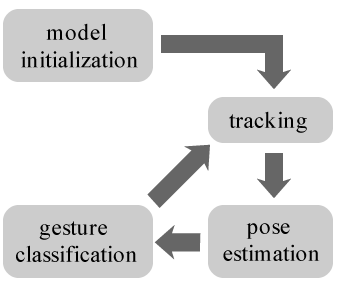
\includegraphics[width=0.3\textwidth]{images/seminar/4steps.png}
\caption{Four main steps in gesture recognition}
\label{fig:4steps}
\end{figure}

%%%-%-%-%-%-%-%-%-%-%-%-%%-%-%-%-%-%-%-%-%-%-%-%%%
%\section{History of gesture recognition}
%\label{sec:history-of-gesture-recognition}

%%%-%-%-%-%-%-%-%-%-%-%-%%-%-%-%-%-%-%-%-%-%-%-%%%
\section{Tracking}
\label{sec:tracking}

The visual tracking techniques in gesture recognition aim at extracting certain features or visual cues for posture estimation and gesture classification. While most of the feature extraction algorithms work principally on images from a single camera \cite{Schmidt}, many setups nowadays use stereoscopic vision from two or more cameras \cite{Chien, VandenBergh}. The depth information gained from stereoscopic vision helps to surpass the big challenge of tracking body parts that are self-occluding in a monocular setting. But stereoscopic vision still has the disadvantage of requiring higher processing speed of the hardware \cite{Schmidt}. %monocular->3dmodel

While most tracking techniques described in this section can be applied in other computer vision problems or gesture recognition applications, which focus on other body parts such as arms, faces or torso, they are also relevant for the gesture recognition topic of tracking hands.

In gesture recognition, tracking mainly consists of the two processes of \textit{figure-ground segmentation} and finding \textit{temporal correspondences} \cite{Moeslund}. Moeslund et al further classify the figure-ground segmentation into five categories: background subtraction, motion based, appearance based, shape based and depth based segmentation.

%------------------------------------------------%
\subsection{Figure-ground segmentation}
\label{sub:figure-ground-segmentation}

\subsubsection{Background segmentation}
The simplest way to separate background from foreground is to take the difference of an empty reference background image and an arbitrary frame. However, this approach is not used, because pixels aren't independent and time-varying background objects should also be considered as background.

In PFinder, Wren et al. \cite{Wren} represented (see figure \ref{fig:pfinder}) each pixel by a Gaussian described by a full covariance matrix, where each pixel is updated recursively with the corresponding statistical properties. This allowed for changes in the background scene like waving curtains or moving objects. The pixels belonging to the figure can then be determined by the Mahalanobis distance. %Moeslund et al. mention that the idea of the mixture of Gaussians (MoG) was introduced by \cite{354}. 
But often the part that needs to be tracked is just a hand or the head in order to further refine a search area. In this case a color cue can be obtained by the same methods.
\begin{figure}[h!]
\center
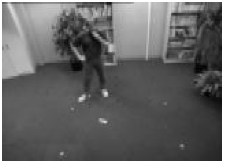
\includegraphics[width=0.4\textwidth]{images/seminar/pfinder1.png}

\includegraphics[width=0.4\textwidth]{images/seminar/pfinder2.png}
\caption{Background segmentation in PFinder \cite{Wren}}
\label{fig:pfinder}
\end{figure}

\subsubsection{Motion based segmentation}
Motion based segmentation does not find temporal correspondences but inspects the difference of two consecutive frames, like Sidenbladh did for the figure-ground segmentation of sequences containing a walking figure \cite{Sidenbladh}. Azoz et al. detect time varying edges as a motion cue to separate edges belonging to the figure from edges in the background.

\subsubsection{Appearance based segmentation}
Using the fact that the appearance of the searched body part can vary from person to person, but is definitively different from the appearance of the background, classifiers can be trained with sets of images containing the appearance of positives and sets with negatives for the background. These classifiers can then be used to detect that type of figure in the scene. Usually, this technique gives no figure-ground segmentation but indicates the location in the scene with a bounding box. 

\subsubsection{Shape based segmentation}
Shape based segmentation often refers to silhouette based segmentation which relies on a good background subtraction. Agarwal and Triggs use silhouettes, because they are easily obtained and because shadowing in the figure, clothing and texture is not encoded in the information. But silhouettes have several disadvantages like occlusion problems or shadow attachments that can distort the shape. 
Takahashi et al. \cite{Takahashi} and Chu and Cohen \cite{Chu} also extract shape from multiple cameras to construct a visual hull of the figure. But shape based segmentation is not always silhouette based: Mori et al. use shapes obtained by edge detection \cite{Mori-a} and in \cite{Mori} by a normalized cuts segmentation in order to identify \textit{salient} limbs \ref{fig:normalizedcuts}, which are later assembled into a posture. Azoz et al. use shape filters to detect clusters of colors \cite{Azoz}. 
\begin{figure}[h!]
\center
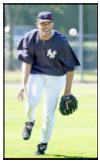
\includegraphics[width=0.2\textwidth]{images/seminar/normalizedcuts1.png}
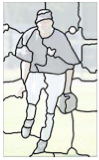
\includegraphics[width=0.2\textwidth]{images/seminar/normalizedcuts2.png}
\caption{Normalized cuts segmentation \cite{Mori}}
\label{fig:normalizedcuts}
\end{figure}

\subsubsection{Depth based segmentation}
Using two ore more cameras, a depth map or a complete three-dimensional reconstruction can be estimated. A depth map \ref{fig:depthmap} can be computed with a disparity map, which is obtained by a correspondence algorithm. Due to the estimation, occlusions or lens geometry problems, depth maps do not always reflect the 3D scene accurately. In \cite{Chien}, Chien et al. refines the accuracy of the correspondence algorithm with epipolar geometry, using the pointing direction from several images.
In \cite{Chu,Takahashi,VandenBergh} silhouettes of the figure from multiple cameras are used to obtain a three-dimensional visual hull with a voxel reconstruction algorithm.
\begin{figure}[h!]
\center
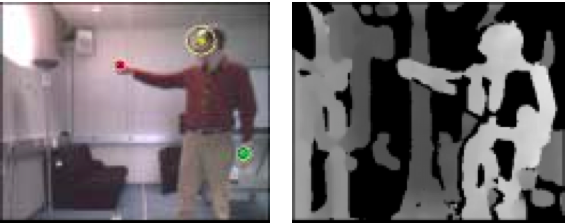
\includegraphics[width=0.8\textwidth]{images/seminar/depthmap.png}
\caption{Scene with estimated depth map \cite{Nickel}}
\label{fig:depthmap}
\end{figure}

%------------------------------------------------%
\subsection{Temporal correspondences}
\label{sub:temporal-correspondences}

Finding the temporal correspondences resolves ambiguities while tracking objects or figures in an image, given their states in past frames. Temporal correspondences can help, when multiple tracked objects occlude each other,  or simply to correctly distinguish two nearby objects.

Commonly, the task of tracking objects across frames is done with an estimator, which first predicts the location of the object for the next frame, based on previous tracking results and secondly reconciles the measured location of the object with the predictions. A broader class of estimators called condensation algorithms, on which the particle filters are based, can also take occlusions into account by representing multiple possibilities as hypotheses or "particles" to predict future locations of the tracked objects.

Schmidt and Fritsch use a kernel based particle filter \cite{Schmidt}, which has the advantage over standard particle filters of avoiding a huge number of particles required for tracking the upper body and arms with 14 degrees of freedom.

%%%-%-%-%-%-%-%-%-%-%-%-%%-%-%-%-%-%-%-%-%-%-%-%%%
\section{Pose estimation}
\label{sec:pose-estimation}

Once the searched limbs or figure features are tracked, pose estimation or model matching adds a layer of abstraction by assembling features into a superstructure which can later be classified. The main goal of pose estimation is to recover an underlying skeletal structure. Moeslund et al. propose a separation of pose estimation methods according to their use of a model \cite{Moeslund}:

%------------------------------------------------%
\subsection{Model-free}
\label{sub:model-free}

Model-free methods do not use a-priori knowledge of the body configuration. The limb or parts are either assembled dynamically or their constellation can be matched to a pose by comparing them to a database of examples.

Agarwal and Triggs presented a method which recovered a 3D pose from monocular images without using manually labeled examples or templates nor using a body model. The pose is estimated by inferring joint angles from silhouettes with a Relevance Vector Machine (RVM) regression \cite{Agarwal}

One of the first model-free pose estimations was PFinder \cite{Wren}. Wren et al. dynamically added blobs to the pose, either by contour matching or a color splitting process. 

Another approach is to dynamically decompose a visual hull into 3D Haarlets (see figure \ref{fig:haarlet}) using Linear Discriminant Analysis (LDA) \cite{VandenBergh} or into shape descriptor atoms with a matching pursuit algorithm and Singular Value Decomposition (SVD) resulting in shape descriptors with the largest eigenvalues \cite{Chu}. Both methods have a key advantage: the atomic shape description and the 3D Haarlets have an additive property (see figure \ref{fig:visualhull}), drastically reducing the number of possible poses to which the measured visual hull can be matched.
\begin{figure}[h!]
\center
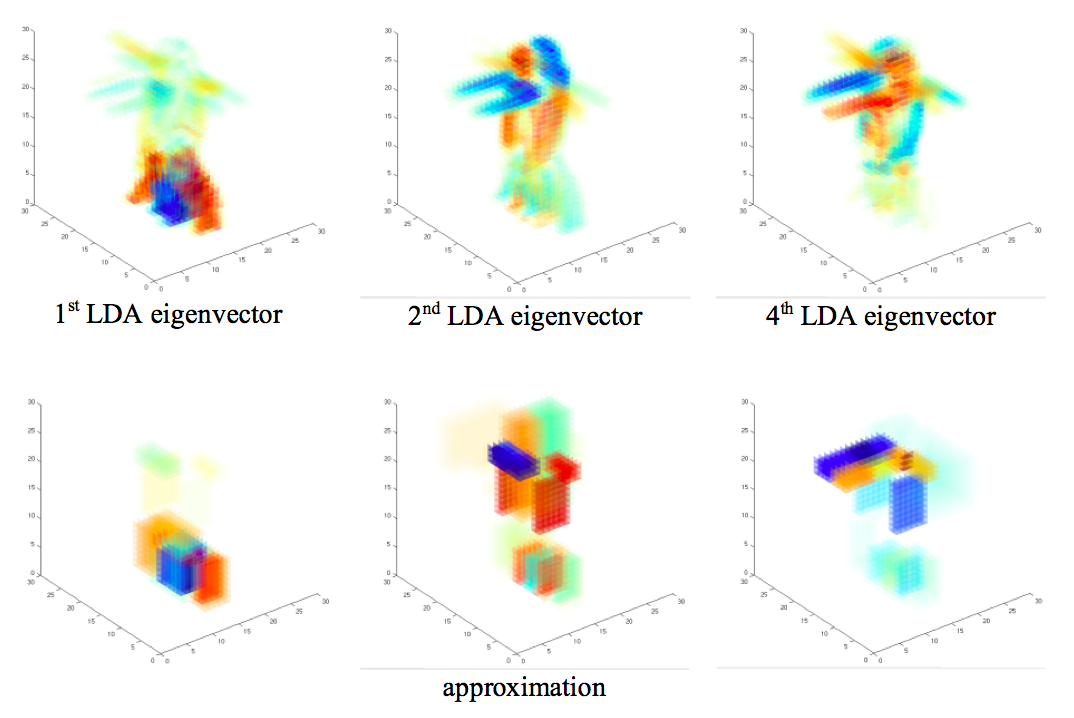
\includegraphics[width=0.8\textwidth]{images/seminar/ldaeigenvectors.png}
\caption{3D Haarlets and their approximation\cite{VandenBergh}}
\label{fig:haarlet}
\end{figure}
\begin{figure}[h!]
\center
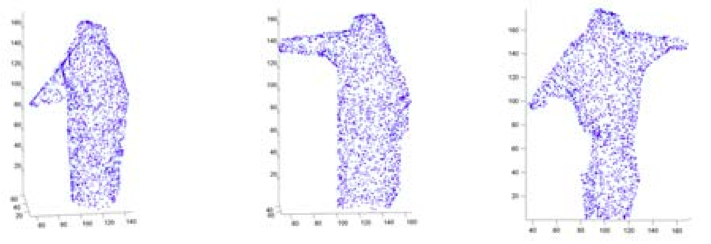
\includegraphics[width=0.8\textwidth]{images/seminar/visualhullcomposition.png}
\caption{Additive property of visual hulls \cite{Chu}}
\label{fig:visualhull}
\end{figure}

%------------------------------------------------%
\subsection{Indirect model use}
\label{sub:indirect-model-use}

This category does not directly map the tracked information onto a model, but rather guides the interpretation. Information like joints, limb length ratios, etc. is labelled into the examples.

Mori et al. use multiple constraints like torso length ratio, adjacency to torso or joints and a-priori body configuration and clothing properties \cite{Mori}. In another approach Mori et al. recover the pose from labelled silhouette examples by deforming the measured shape and therein the skeletal structure to match the labelled example \cite{Mori-a} (see figure \ref{fig:deformable}).
\begin{figure}[h!]
\center
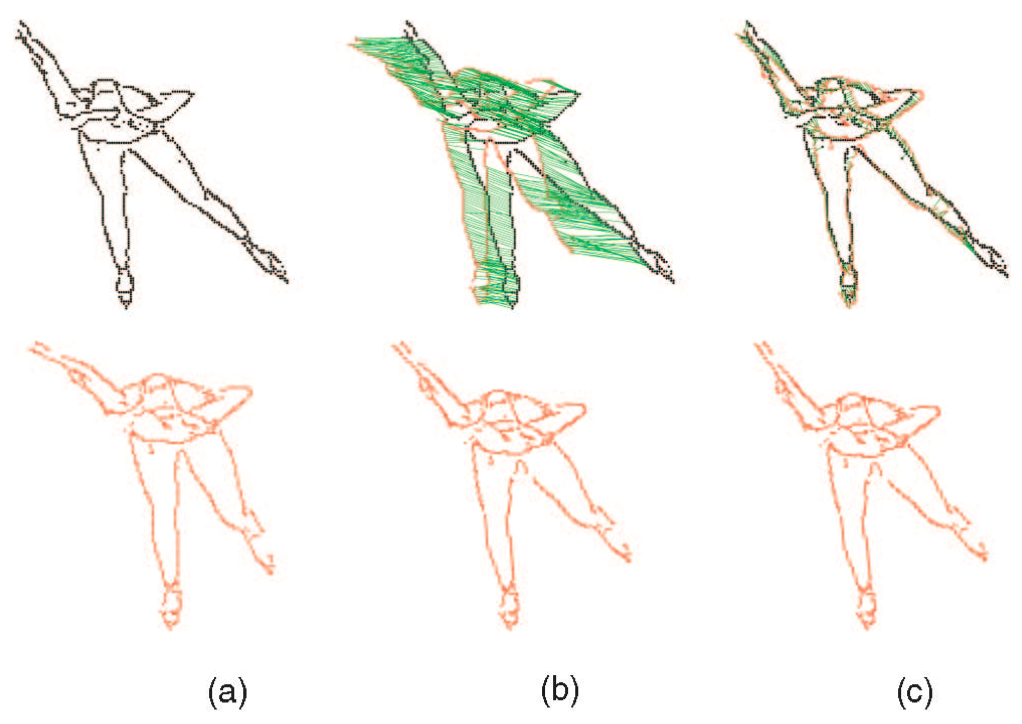
\includegraphics[width=0.8\textwidth]{images/seminar/shapecontextmatching.png}
\caption{Deformable shape context matching \cite{Mori-a}}
\label{fig:deformable}
\end{figure}

%------------------------------------------------%
\subsection{Direct model use}
\label{sub:direct-model-use}

With the direct model approach, the geometric representation of the figure is known beforehand, and the measured data is matched against the model. In newer approaches the model contains human motion constraints to further eliminate ambiguities.

Bray et al. use a smart particle filter (SPF) to fit the tracked results on to a hand model with 15 degrees of freedom and modelling the hand surface in 3D \cite{bray} while respecting the physical model constraints. 
\begin{figure}[h!]
\center
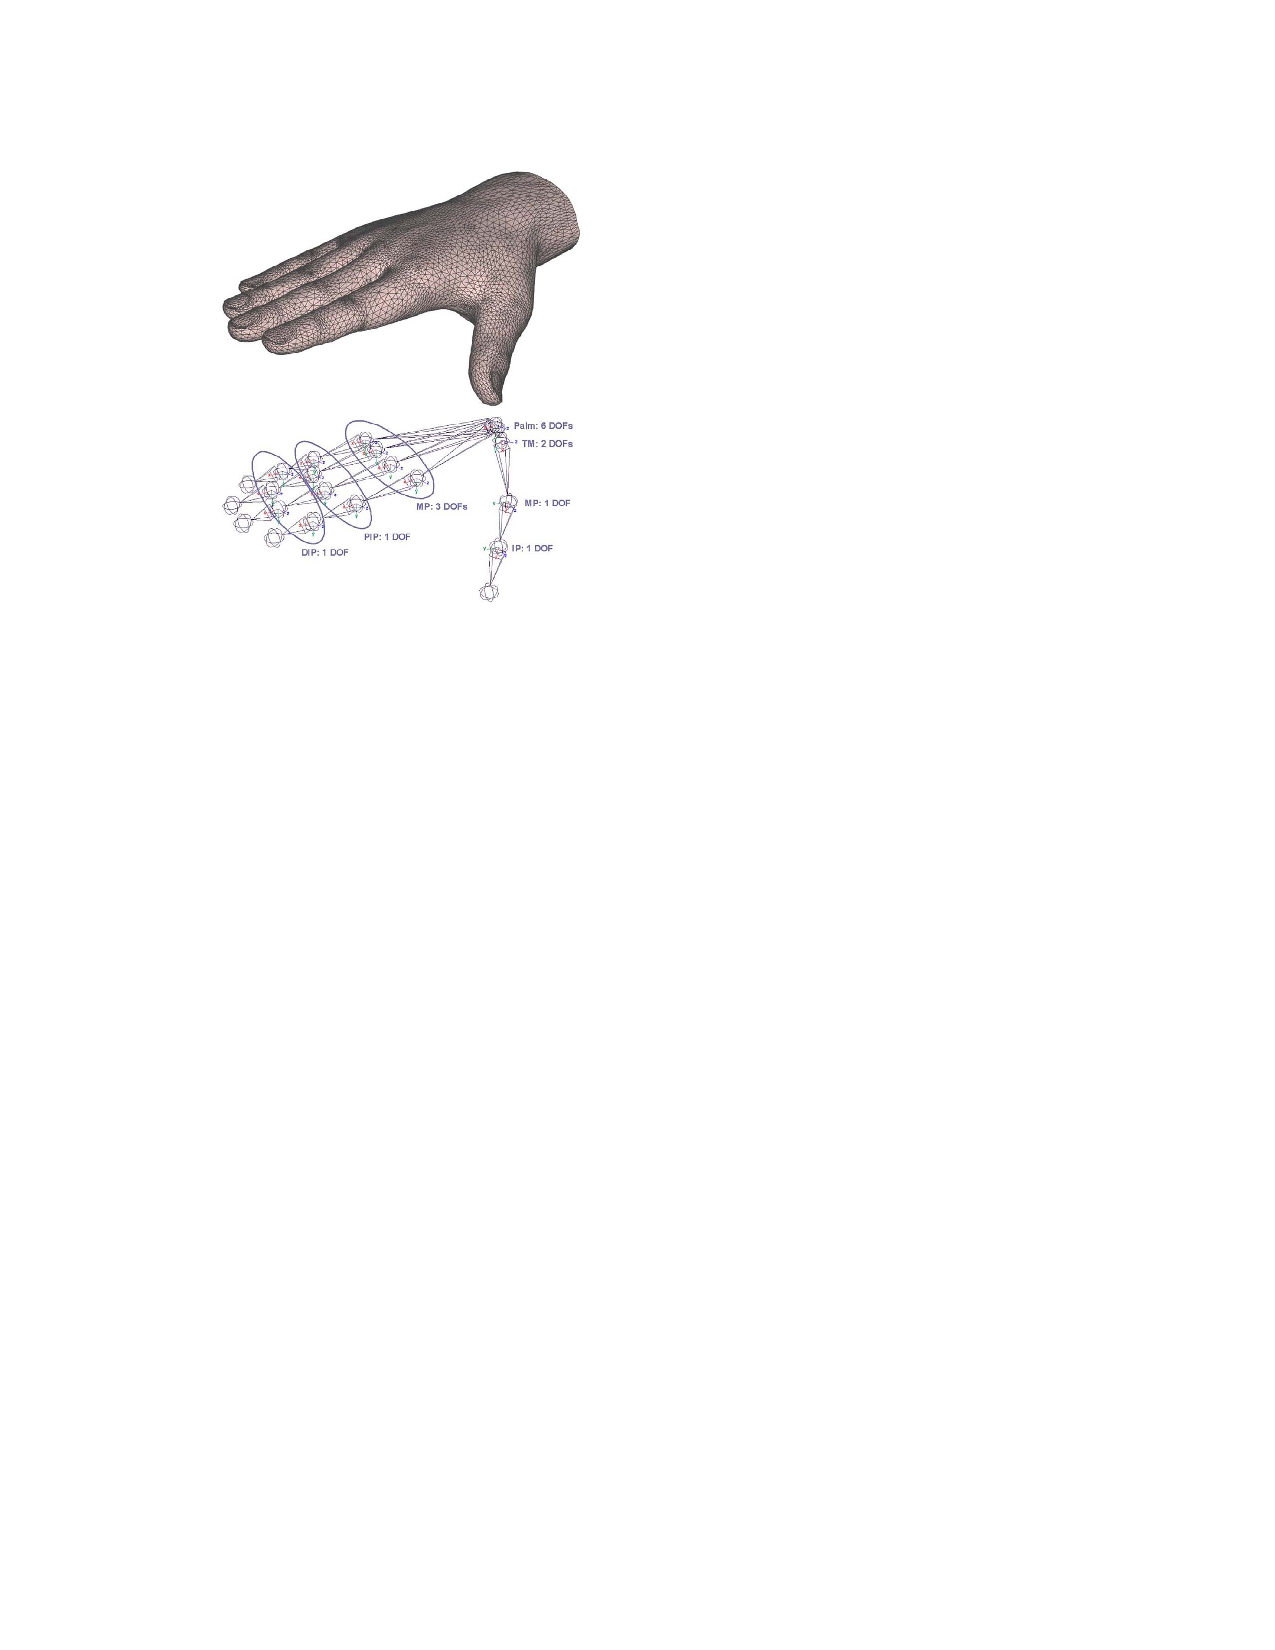
\includegraphics[width=0.5\textwidth]{images/bray_gool_handmodel}
\caption{Hand model as polygonal surface and its skeleton with 15 degrees of freedom \cite{bray}}
\label{fig:bray-gool-hand}
\end{figure}

%%%-%-%-%-%-%-%-%-%-%-%-%%-%-%-%-%-%-%-%-%-%-%-%%%
\section{Recognition}
\label{sec:recognition}

There are several approaches to classify gestures, depending on what information to classify. Because gestures can be viewed as sequence of postures in time, the most widely used classification method is a Hidden Markov Model (HMM). HMMs are suited for the classification of gestures, they try to model the spatio-temporal variability and to maximize the likelihood of generating all examples of a gesture class \cite{Yang}.
 
Yang et al. trained a HMM for spotting specific body gestures like raising a hand, jumping etc., but also presented the concept of the garbage gesture model (see figure \ref{fig:garbage}) and the key gesture spotting model (see figure \ref{fig:gesturespotter}). The garbage gesture model is an ergodic model and tied in the the key gesture spotter model at the beginning of a gesture and at the end \cite{Yang}.
\begin{figure}[h!]
\center
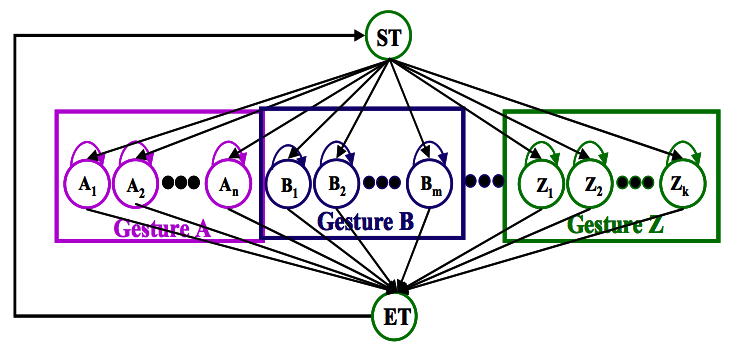
\includegraphics[width=0.5\textwidth]{images/seminar/garbage.png}
\caption{Garbage gesture model \cite{Yang}}
\label{fig:garbage}
\end{figure}
\begin{figure}[h!]
\center
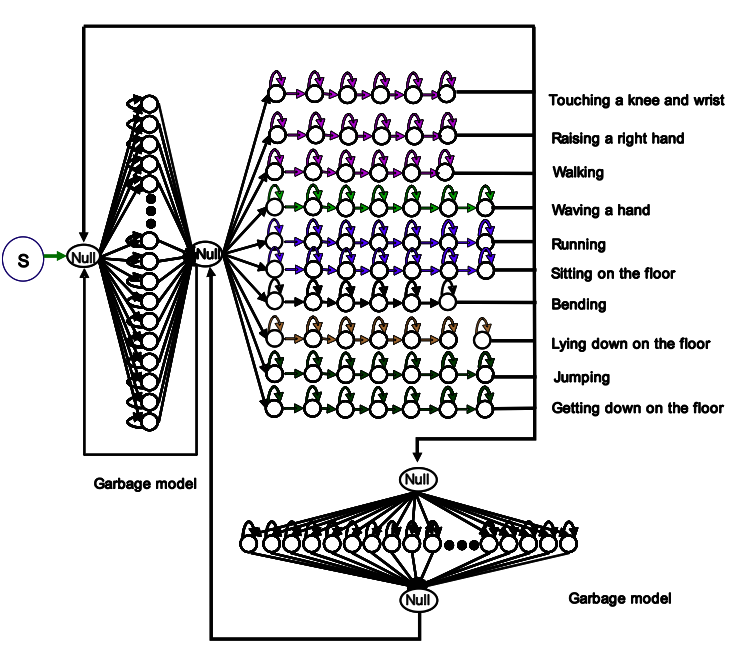
\includegraphics[width=0.6\textwidth]{images/seminar/gesturespotter.png}
\caption{Key gesture spotter model \cite{Yang}}
\label{fig:gesturespotter}
\end{figure}

Both Willson et al. and Chu and Cohen used the concept of a multiphasic gesture: in a sequence of postures, there is at least a transition to the key posture and a transition leaving it. Gestures can also have several key postures identifying a gesture. While Willson et al. did not use hidden states but a simpler markovian chain, Chu and Cohen used a dual-state HMM for a primary and secondary decomposition of gestures, which also gives smaller set of atoms and a HMM state space of linear complexity \cite{Chu,Wilson}.

Wang et al. introduce a powerful approach for gesture classification: hidden conditional random fields (HCRF) (see figure \ref{fig:hcrf}). HCRFs incorporate hidden states variables in a discriminative multi-class random field. It is an extension of the spatial Conditional Random Fields and takes the main advantage of HMMs, the capability of modelling temporal sequences. HCRFs can be used like HMMs (see figure \ref{fig:hmm}), but the hidden states can be shared among different gesture classes \cite{Wang}. 
\begin{figure}[h!]
\center
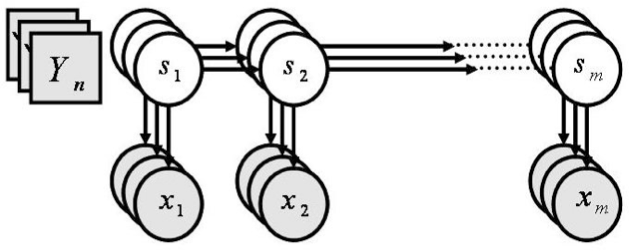
\includegraphics[width=0.45\textwidth]{images/seminar/hmm.png}
\caption{Hidden Markov Model \cite{Wang}}
\label{fig:hmm}
\end{figure}
\begin{figure}[h!]
\center
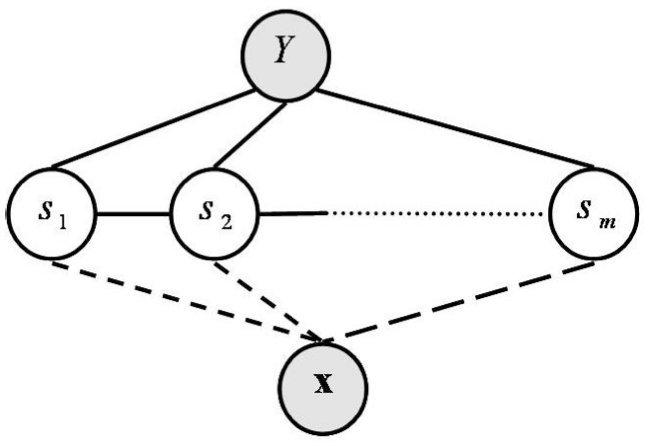
\includegraphics[width=0.3\textwidth]{images/seminar/hcrf.png}
\caption{Hidden Conditional Random Field \cite{Wang}}
\label{fig:hcrf}
\end{figure}

%\subsection{Hidden markov models}
%\label{sub:hidden-markov-models}

%\subsection{Bayesian networks}
%\label{sub:bayesian networks}

%%%-%-%-%-%-%-%-%-%-%-%-%%-%-%-%-%-%-%-%-%-%-%-%%%
%\section{Current development}
%\label{sec:current-development}

%After this general overview of the steps generally used in gesture recognition, the field of hand recognition has something something.

%particlefilter
%->mit

\section{Our approach}
\label{sec:our-approach}

Erol et al. \cite{hand-review} mention the difficulties in hand gesture recognition: 
\begin{itemize}
\item high-dimensional problem
\item self-occlusion
\item uncontrolled environment
\item rapid hand movements
\item processing speed
\end{itemize}
There is an approach from Wang and Popovic from MIT, where the processing requirements are circumvented by generating a nearest neighbours lookup database for scaled-down 40$\times$40 pixel images of a color marked glove (see figure \ref{fig:mit}) \cite{mit}.
\begin{figure}[h!]
\center
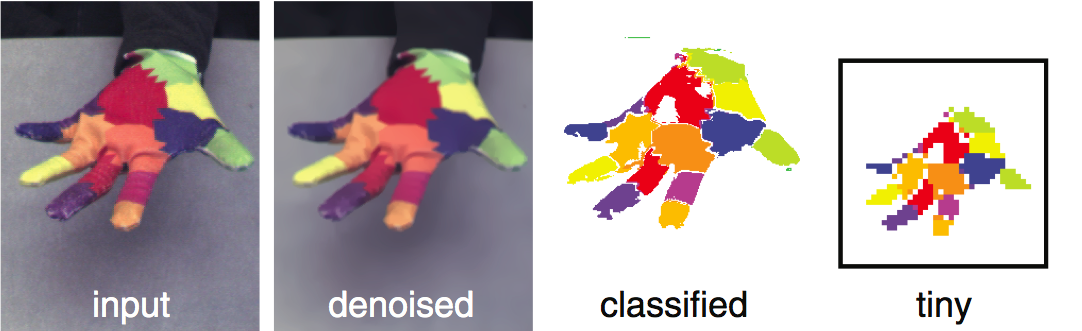
\includegraphics[width=0.6\textwidth]{images/mit}
\caption{Pose estimation with a color-marked glove and its 40$\times$40 pixels representation (tiny) \cite{mit}}
\label{fig:mit}
\end{figure}

However many tracking algorithms widely used in gesture recognition are confronted with real-time problems. Preliminary tests with advanced algorithms have been done in OpenCV \cite{opencv} -- a computer vision library that includes over 500 algorithms from research -- using optical flow algorithm or background subtraction with mixtures of gaussians. While the results are real-time capable for smaller images, the frame-rate often drops to under 10 frames per second for bigger images.

Our approach aims at using simple techniques focusing on speed with some constraints limiting the scope of the project and still having an architecture where an real-time ergonomic gestural  interface is possible.
%realtime focus
%%%%%%%%%%%%%%%%%%%%%%%%%%%%%%%%%%%%%%%%%%%%%%%%%%
\chapter{Setup and frameworks}
\label{chap:setup-and-frameworks}

Following the overview of existing gesture recognition techniques in the previous chapter (chapter \ref{chap:gesture-recognition}), this chapter focuses on the hardware and software requirements necessary for implementing a gesture recognition architecture. These requirements will lead to a choice of hardware components and of an ensemble of software libraries to be used in this project. Since there are many software libraries capable of performing the individual tasks of tracking or classification, but not all of them are suited for a real-time-capable integrated architecture, the choice of camera, environment constraints and libraries is greatly influenced by the main requirement of the real-time, or quasi-real-time component of ergonomic gestures.

%%%-%-%-%-%-%-%-%-%-%-%-%%-%-%-%-%-%-%-%-%-%-%-%%%
\section{Hardware}
\label{sec:hardware}

The main task of the hardware is to see a user's hand and fingers positions and movements while this user is sitting in front of the interface. While there are approaches based on accelerometer and gyroscopic sensors 
\cite{dataglove}, this project will focus on a vision-based setup and will therefore use a camera. The interface can be anything from an LCD display to a beamer, as long it is in front of the user and not obstructing the field of view of the camera. In order for a camera to \textit{see} the fingers, several important requirements have to be met for the camera:

\begin{itemize}
\item Resolution: \\ The camera frame must contain enough information about the fingers in order to localize and distinguish them from each other. As ad-hoc tests have shown, resolutions of 320$\times$240 pixels may work, depending of the user's action space and the distance between the camera and the user, but often overstep the threshold of being distinguishable or simply the threshold of detection of the fingers.

\item Frame rate: \\ Even if the recognition of a gesture can operate at a much lower sampling rate while still having enough consecutive samples to identify a gesture reliably (in the range of 5 to 20 frames per second), the articulated and sudden or rapid movements of the hand result in blurred fingers in a single frame taken at up to 30 frames per second \cite{blurry}. Therefore, the camera should acquire the images at a speed where rapid movements can be captured without motion blur (even if each second or third frame will be skipped in the video processing loop).

\item Color and image fidelity: \\ Movements of hands and fingers should not result in distorted images often seen in conventional web-cams. In order to prevent difficulties in the tracking algorithms, the 
camera should have low color shifts and a low noise ratio;
\end{itemize}

Given a camera that meets these requirements and providing a solid basis for the video processing steps, this project further constrains the goal regarding the tracked object: in order to meet the requirement of being able to localize the finger positions in a given image, the user is wearing a glove with marked finger extremeties.

%------------------------------------------------%
\subsection{Camera}
\label{sub:camera}

While most of the conventional USB Web-cameras do not meet the camera requirements established above, the following three cameras, often used in computer vision systems, do.
\begin{itemize}
\item Point Grey FireFly MV (752$\times$480 at 60 FPS) \cite{pointgrey}
\item Unibrain Fire-i (501 Model: 640$\times$480 at 86 FPS) \cite{unibrain}
\item Sony PS3 Eye (640$\times$480 at 75 FPS) \cite{ps3eye}
\end{itemize}

While each of these cameras could be used in this project, the choice fell on the Sony PS3 Eye camera (see figure \ref{fig:ps3-eye}). Its main advantage is its cost, subsidized by Sony for the use with Playstation games, which is under CHF 70.- in most electronics stores.

\begin{figure}[H]
\center
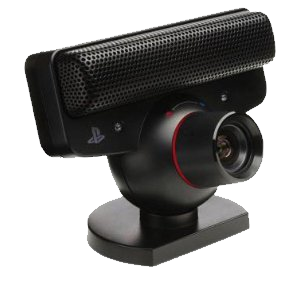
\includegraphics[width=0.3\textwidth]{images/ps3eye} 
\caption{Sony PS3 Eye camera}
\label{fig:ps3-eye}
\end{figure}

While Sony does not provide a driver, a member of the Natural User Interface group \cite{nuigroup} provided a Windows driver that supports frame rates up 75 FPS in VGA (640$\times$480) resolution and up to 120 FPS in QVGA (320$\times$240) resolution \cite{codelab}. The driver is also capable of grabbing frames from multiple cameras in OpenCV under Windows, which could be a requirement for stereoscopy, whereas under other Operating Systems, only one camera was recognized in OpenCV.
 
%------------------------------------------------%
\subsection{Glove}
\label{sub:glove}

The use of a glove facilitates the tracking of the fingers: for the scope of this project, tracking color-based markers on the fingertips presented a acceptable shortcut to obtain the finger positions. \\
The glove was initially designed to put it on and off quickly, without having the disadvantage of placing all the color markers each time on the hand. The design also went through several versions optimizing the placement and color of the markers for better tracking results (see figure \ref{fig:glove}).
The main improvement was obtained by placing the markers on the fingertips in a way that did not cover the whole circumference of the finger, which provided the ability to distinguish the fingers for the tracking phase.

\begin{figure}[H]
   \centering
   \subfloat[1$^{\text{st}}$ version]{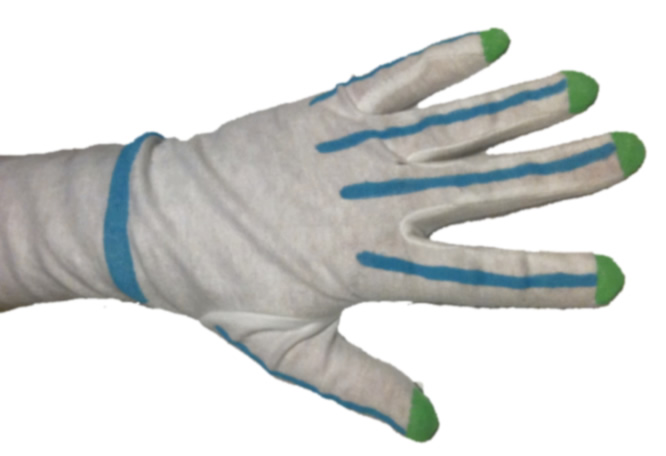
\includegraphics[width=0.25\textwidth]{images/glovev1}}
      \hspace{0.05\textwidth}
   \subfloat[2$^{\text{nd}}$ version]{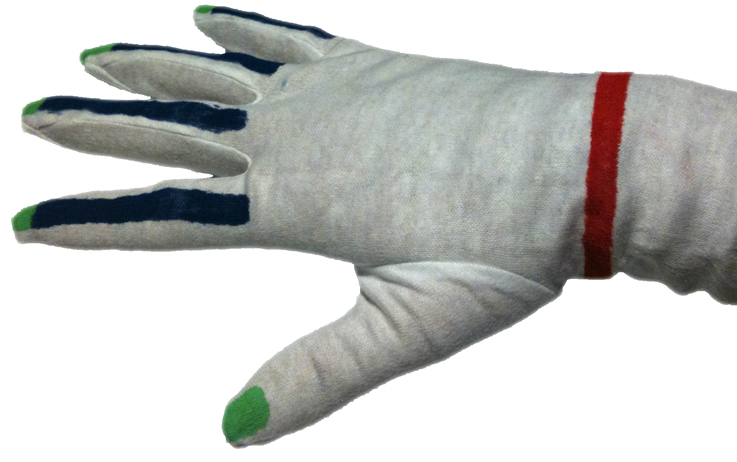
\includegraphics[width=0.25\textwidth]{images/glovev2}}
   	\hspace{0.05\textwidth}
   \subfloat[3$^{\text{rd}}$ version]{
\includegraphics[width=0.25\textwidth]{images/glovev3}}
   \caption{Color-marked textile glove}
   \label{fig:glove}
\end{figure}

%------------------------------------------------%
\subsection{Environmental constraints}
\label{sub:environmental-constraints}

Initially, the following setup had been proposed:
\begin{itemize}
	\item the user is sitting in front of the interface,
	\item while sitting and resting the elbows on the table,
	\item and the camera being placed at a distance where the gestural action space is contained in the field of view of the camera (see figure \ref{fig:setup}).
\end{itemize}

\begin{figure}[H]
\center
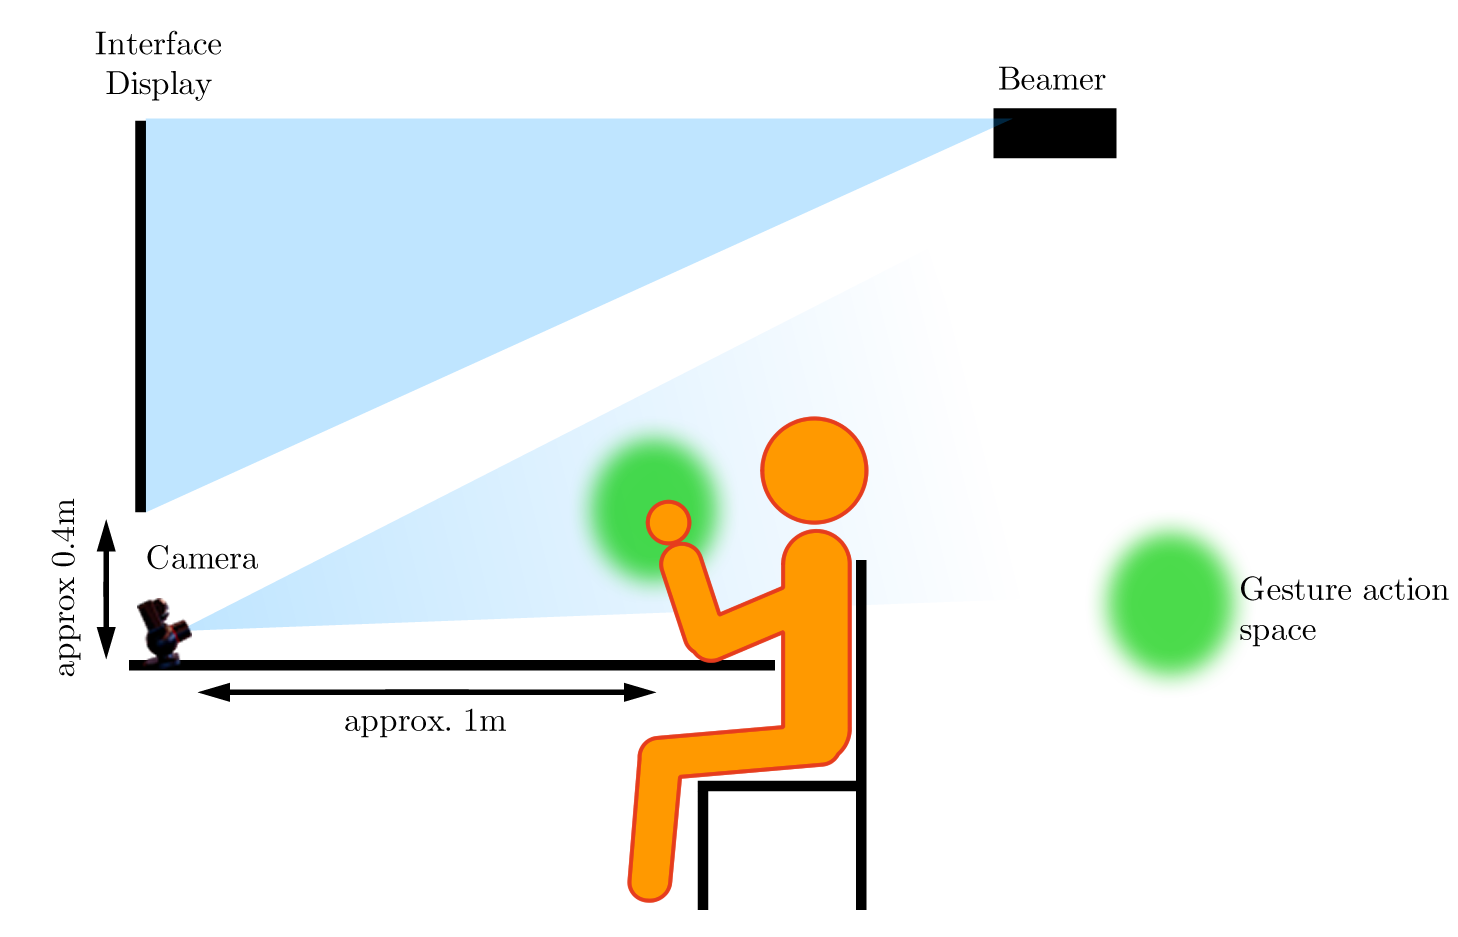
\includegraphics[width=0.9\textwidth]{images/setup} 
\caption{Setup of the interface}
\label{fig:setup}
\end{figure}

While this project aims at recognising hand postures and gestures without too much restricting the setup, some constraints have to be further imposed in order to reliably obtain good tracking and classification results. 

Even if the tracker algorithm operates in a color space that is less dependent of the luminance of the color like HSL or Lab color space, there are some limits due to the gain of the camera: in a very dim lit environment the noise is too much amplified by the gain and the colors are more indistinguishable. Equally, with very bright spots or in direct sunlight, the pixels of the color markers lose their color information, turning to a color value close to white.

The glove's design was optimized for frontal control gestures. The placement of the wrist marker imposes a further environmental constraint: the camera has to be placed lower than the display, allowing it to film in a slightly rising direction and ensuring to capture the wrist markers whenever executing a gesture. But of course color markers on the glove also means that neither the user nor the background can contain these colors.

%%%-%-%-%-%-%-%-%-%-%-%-%%-%-%-%-%-%-%-%-%-%-%-%%%
\section{Software}
\label{sec:software}

The main requirement of the software is to allow real-time tracking and classification. To this regard, the tracking and classification algorithms should be written in C/C++. Of course, other languages might be viable for real-time image processing algorithms, capable of managing threads and offering helping mechanisms like a garbage collector. But initial library tests have shown, especially for image processing algorithms, that with a slightly heightened awareness for memory management, thread management and algorithm execution times, better performances could be achieved more easily with C/C++.

%------------------------------------------------%
\subsection{Overview}
\label{sub:overview}

A library or set of libraries is needed, where the following tasks are covered:

\begin{itemize}
\item fast image processing algorithms
\item ability to train a classifier
\item easily design a performant GUI for rapid application development
\item take advantage of a multicore hardware architecture
\end{itemize}

Due to the chosen hardware (see section \ref{sub:camera}) for which the device driver operates best in the Windows operating system, the choice of the development environment falls to the Visual Studio 2008 IDE. 

%------------------------------------------------%
\subsection{Libraries and frameworks}
\label{sub:libraries-and-frameworks}

\subsubsection{OpenCV}
OpenCV \cite{opencv} is a library containing a large set of algorithms covering computer vision and machine learning tasks. It is a cross-platform library initially developed by Intel and now maintained under active development by Willow Garage \cite{opencv-web}. Its goal was to advance computer vision research and provide a basic infrastructure for computer vision. This library was chosen for its focus on real-time image processing.
The current version is 2.2, however this project used the version 2.0, because at the time of the first integration of the OpenCV algorithms, the tracking was optimized for multithreading using OpenMP instructions. OpenCV abandoned its built-in OpenMP optimizations in favour of TBB (Thread Building Blocks).

\subsubsection{dlibc++}
The dlib library \cite{dlib} was chosen for its well documented usage of Support Vector Machines (SVM). It provides a C++ API for a multitude of binary classifiers and regression tools: Relevance Vector Machines (RVM), kernel recursive least squares (KRLS), kernel ridge regression (KRR) and several implementations of Support Vector Machines.

\subsubsection{QT}
QT \cite{qt} was favored over Windows forms (.NET or MFC) because of the extension possibilities like the integration of OpenGL within QT widgets. The use of OpenGL to display enhanced video frames greatly improves the performance in combination with an OpenGL capable graphics hardware. Furthermore it is an multi-platform and open-source GUI framework.

\subsubsection{libconfig}
Initially the tracker program featured Boost object serialization for saving the states and parameters of the image processing steps. But due to consistency problems a simpler solution was needed. libconfig is a library for reading and writing structured configuration files, with type-awareness, groups, lists, arrays, strings and numbers.


\chapter{Chosen gestures}
\label{chap:chosen-gestures}

This chapter introduces the gestures that this project aims to recognize. The establishement of a ground truth is discussed in section \ref{sec:wizard-of-oz-experiment} and the selected gestures for this project presented in section \ref{sec:gestures}.

\section{Wizard of Oz experiment}
\label{sec:wizard-of-oz-experiment}

In collaboration with Caroline Biewer and Thomas Holdener writing a master thesis in psychology \cite{psychology} a setup was designed, where probands of a Wizard of Oz experiment would sit in front of a beamer screen and control an application (Google Earth and Powerpoint) through gestures (see figure \ref{fig:survey}). In this setup the probands were recorded in stereo according to the environmental constraints established in section \ref{sub:environmental-constraints} and wearing two gloves of the first version. This study had the goal of analyzing movements with regard to the comprehensiveness, comfort and learnability of their use in a usability evaluation. For this, the illusion of a working gesture recognition system was created, where in fact the "wizard of oz" was directly controlling the application with the keyboard and the mouse. The ergonomic gestures project helped provide this illusion by positioning two PS3 cameras in front of the probands and let them wear the color-marked gloves.

The stereoscopic recordings were intended to be used as a ground truth as well as to determine wich types of gestures were preferred for controlling a visual application. Unfortunately, due to unfavorable lighting conditions and several redesigns of the glove, the recordings were incompatible with later versions of the Ergonomic Gestures Recognition architecture.
\begin{figure}[H]
   \centering
   \subfloat{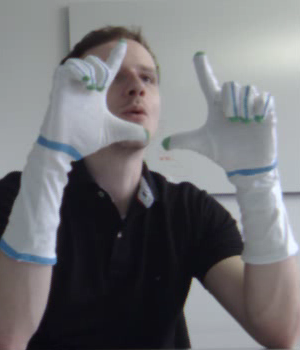
\includegraphics[width=0.235\textwidth]{images/survey1}}
      \hspace{0.01\textwidth}
   \subfloat{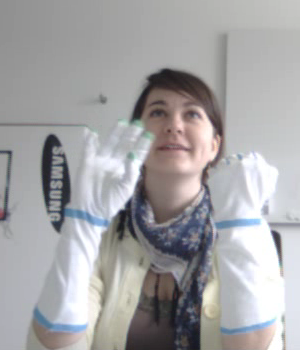
\includegraphics[width=0.235\textwidth]{images/survey2}}
      \hspace{0.01\textwidth}
   \subfloat{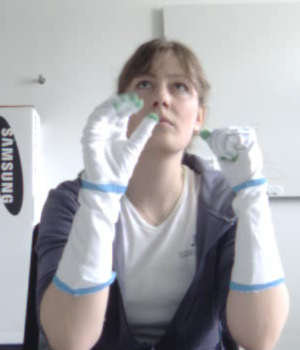
\includegraphics[width=0.235\textwidth]{images/survey3}}
      \hspace{0.01\textwidth}
   \subfloat{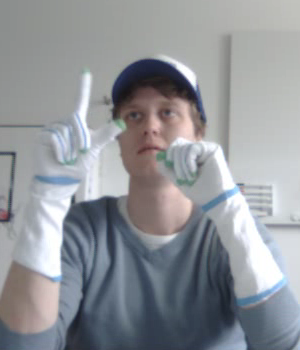
\includegraphics[width=0.235\textwidth]{images/survey4}}
   \caption{Participants performing gestures}
   \label{fig:survey}
\end{figure}

\section{Gestures}
\label{sec:gestures}

After several glove redesigns and the use of monocular videos instead of stereoscopic videos, this project focused to recognize the following gestures, performed by the right hand:
\begin{itemize}
\item Pointing gesture: Index finger pointing upwards, other fingers contracted but with visible markers
\item Zooming gesture: Index an thumb finger pointing upwards, zoom line between index and thumb more horizontal than vertical
\item Horizontal swiping gesture: swiping motion mostly carried out by wrist, not the whole arm.
\end{itemize}

\begin{figure}[H]
	\centering
	\subfloat[Pointing]{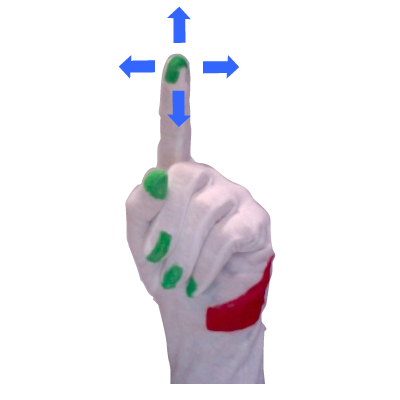
\includegraphics[width=0.22\textwidth]{images/gesture_pointing}}
	\hspace{0.03\textwidth}
	\subfloat[Zooming]{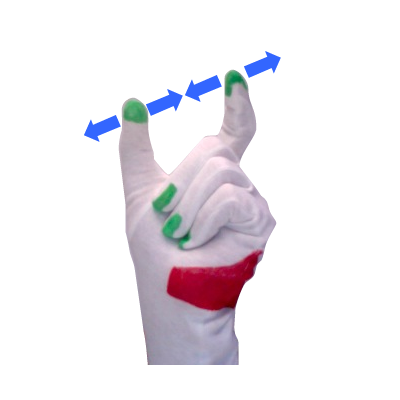
\includegraphics[width=0.22\textwidth]{images/gesture_zooming}}
	\hspace{0.03\textwidth}
	\subfloat[Swiping]{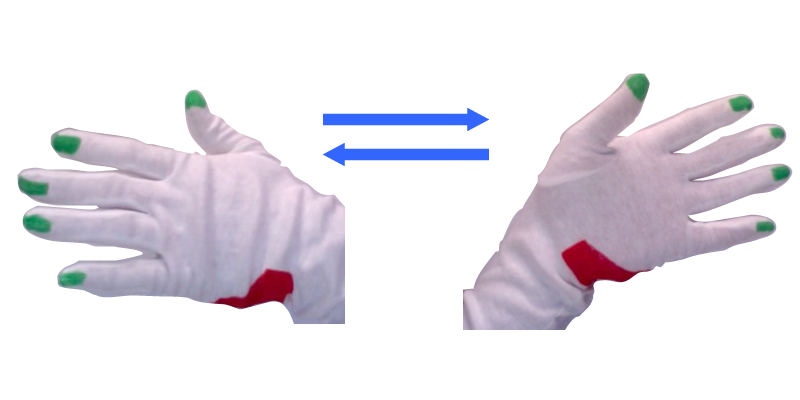
\includegraphics[width=0.44\textwidth]{images/gesture_swiping}}
	
	\caption{Gestures with motions labeled as arrows}
	\label{fig:gestures}
\end{figure}

These gestures were recorded in different videos containing all three gestures with no particular order and containing a single type of gesture repeated several times. In each video the gestures were performed exactly according to the specifications, but while trying maximize the wrist position variability.

%%%%%%%%%%%%%%%%%%%%%%%%%%%%%%%%%%%%%%%%%%%%%%%%%%
\chapter{Design and implementation}
\label{chap:design-and-implementation}

This chapter describes the architecture and implementation of the EGR project. The general three phases for gesture recognition, namely tracking, pose estimation and gesture classification, represents also the basis for this project (see chapter \ref{chap:gesture-recognition}). Using the camera, the glove and the software libraries presented in chapter \ref{chap:setup-and-frameworks}, an architecture that aims at recognizing the gestures chosen in chapter \ref{chap:chosen-gestures} is presented in section \ref{sec:architecture}. In the sections \ref{sec:tracker-configuration}, \ref{sec:model-mapping} and \ref{sec:training-and-classification} implementation details of the tracking phase, the pose estimation phase and the classification phase are presented.

%%%-%-%-%-%-%-%-%-%-%-%-%%-%-%-%-%-%-%-%-%-%-%-%%%
\section{Architecture}
\label{sec:architecture}

The separation of the three gesture recognition phases into separate but linked modules allows a better understanding of the mechanisms involved and offers the possibility to replace a module by an alternate future version, which accomplishes the same task. 
There are two main modules and three applications: 
\begin{itemize}
	\item Tracking module
	\item Model module
	\item Recorder application
	\item Training application
	\item Demo application
\end{itemize}

The tracking module is implemented as a C library, which runs a continuous loop in a thread, and performs the image transformations and blob detection algorithms for each new frame from a video source. The hand model module is implemented as a C++ class object, which maps the information obtained from the tracker in a defined structure and optionally can classify a posture, assuming a decision function obtained from the training application is present. This hand object can then be directly instantiated in a potential gesture recognition application and initialized with the necessary information.


\begin{figure}[H]
\center
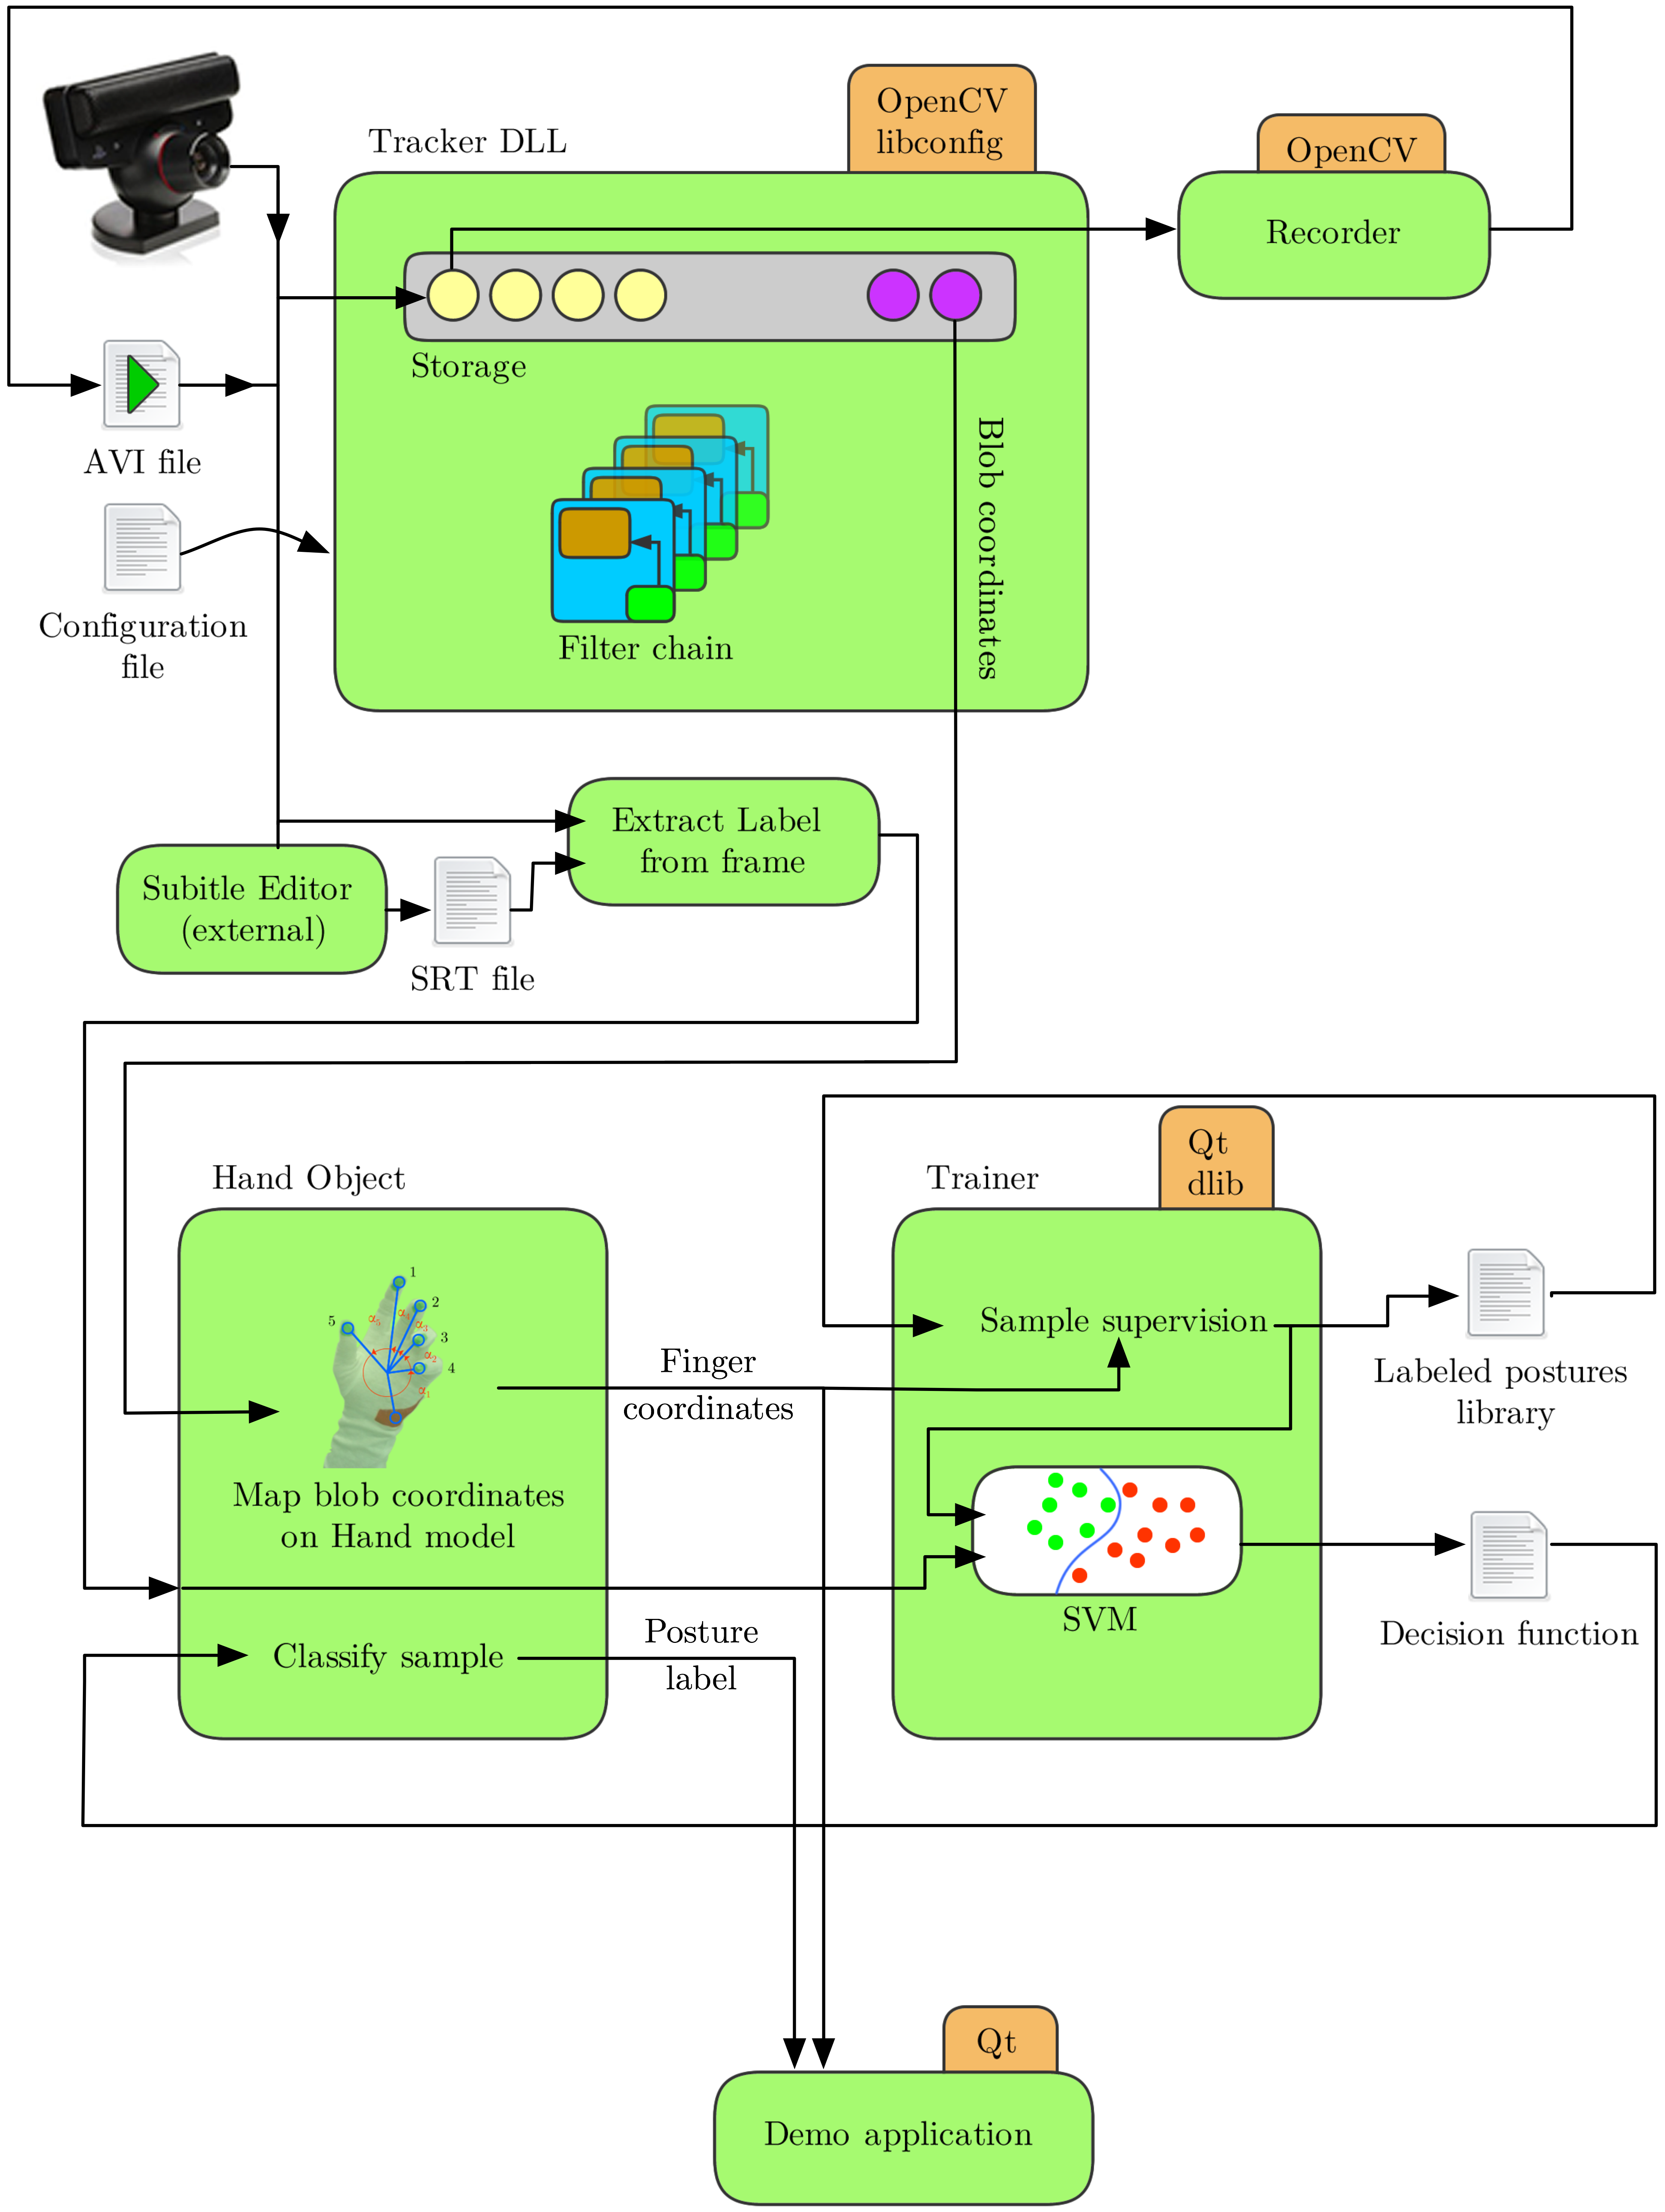
\includegraphics[width=1\textwidth]{images/arch} 
\caption{General architecture of the Ergonomic Gestures Recognition system}
\label{fig:architecture}
\end{figure}

%%%-%-%-%-%-%-%-%-%-%-%-%%-%-%-%-%-%-%-%-%-%-%-%%%
\section{Tracker configuration}
\label{sec:tracker-configuration}

The tracker module is implemented as a library that can be dynamically linked from an another program. This tracker is optimized for speed: it has to run several image processing filters for each frame and achieve a reasonable frame-rate of 10 to 30 FPS. However the frame-rate depends entirely on the optimizations of each image processing algorithm.

The tracker consists of three parts: a storage object, a filter chain and a camera thread. The camera thread acquires the images from the PS3 Eye camera at 60 frames per second in a separate thread. 

The storage object is a simple key-value storage, or more precisely a "key-anything" storage. Its only purpose is to eliminate the need to supervise each allocation and release of memory for the images at each iteration of the filter chain. It has also locking mechanisms implemented to ensure data consistency when an external thread accesses the memory in the storage object. The storage object is accessible from everywhere in the tracker: for example in the initialization phase, the camera descriptors are stored in it, but each image processing algorithm can also access it for its own purposes.

%------------------------------------------------%
\subsection{Filter chain}
\label{sub:filter-chain}

The filter chain allows an arbitrary configuration on how the image processing algorithms are linked. Each element in the chain, called step, can have one image processing algorithm, called filter, associated to it.
Each step has also an overlay object, that can, whenever it is displayed, adjust the parameters and specify the input images of the filter. The filter object itself declares how many input images it needs, and upon executing its function returns a result image. These resulting images can now be used as input images, or sources, to each filter (see figure \ref{fig:chain-general}).

\begin{figure}[H]
\center
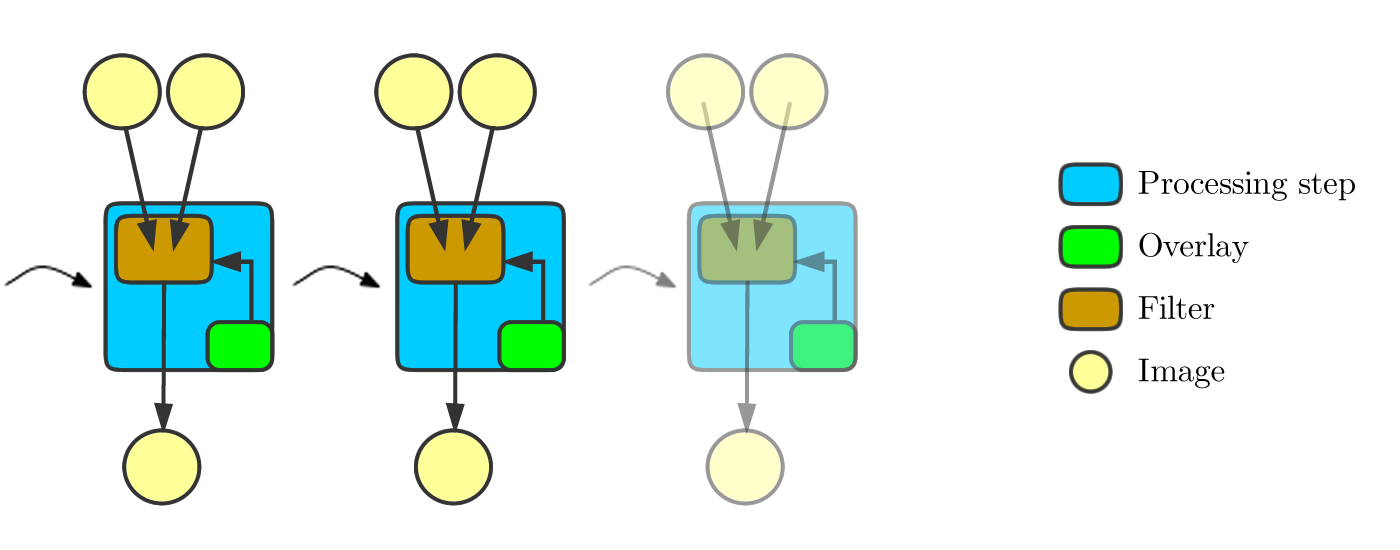
\includegraphics[width=0.9\textwidth]{images/steps} 
\caption{Image processing chain with reconfigurable processing steps: the filter and source image(s) can be specified using the overlay object belonging to the step. }
\label{fig:chain-general}
\end{figure}

The execution of the filter chain is sequential, but the specification of the input sources allow an arbitrary and reconfigurable order of image processing operations. 
To improve the execution speed, there is no GUI control elements used from QT or the built-in OpenCV GUI controls. Instead the user interface is directly in overlay mode with the result image of the selected step (see figure \ref{fig:lab-overlay}).

\begin{figure}[H]
\center
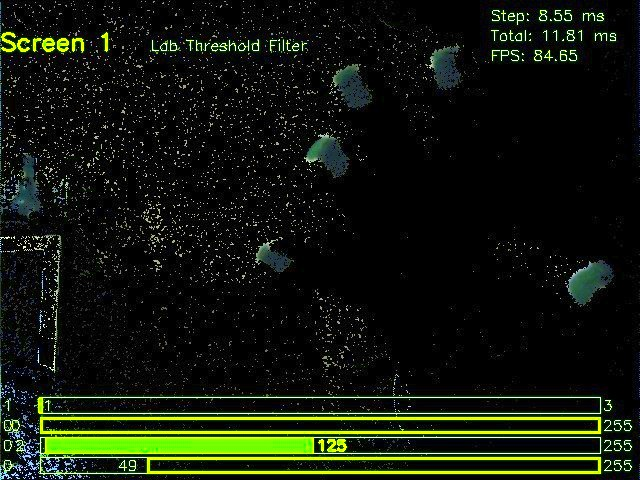
\includegraphics[width=0.7\textwidth]{images/step_lab} 
\caption{Lab threshold filter with overlay interface}
\label{fig:lab-overlay}
\end{figure}

As mentioned in \ref{sec:tracker-configuration}, each filter has access to the global storage object, and can store temporary images in it, but also other objects like vectors containing the positions of the detected blobs. Knowing the identifying key to this vector of points, an external program linked to the tracker DLL can retrieve this information.

%------------------------------------------------%
\subsection{Image processing filters}
\label{sub:image-processing-filters}

The tracker provides a small but easily extensible list of filters:
\begin{itemize}
\item Lab threshold: convert from the RGB color space to the Lab color space, and threshold each plane with a value range.
\item RGB threshold: threshold each RGB plane with a value range.
\item Binary threshold: converts an image into a gray image if needed, and performs a binary threshold.
\item Erosion: convolution directly implemented in OpenCV with a 3$\times$3 kernel.
\item Dilation: convolution directly implemented in OpenCV with a 3$\times$3 kernel.
\item Gaussian smooth: : convolution directly implemented in OpenCV with a gaussian kernel.
\item Add: overlays non-zero parts of a first source image onto a second source image.
\item Blob detection (see below)
\item Fast corner detection (see below)
\end{itemize}

The blob detection and the fast corner detection filters use external algorithms, but the others are implemented with OpenCV functions. The blob detection filter uses the cvBlobsLib available at the OpenCV Wiki \cite{cvblobslib}. The blob detection itself is based on the linear-time component labeling algorithm using contour tracing technique by Chang et al. \cite{blobs}. Tests have shown, that this algorithm performs well, as long the number of blobs remains small. However when the color thresholding filter and the erosion filter leave enough noise in the resulting image, the blob detection algorithm takes up to a second and thus impeaching the fast real-time execution. 
In order to circumvent this possible delay, other detection algorithms were investigated. The most promising was the FAST corner detection algorithm from Rosten and Drummond \cite{fast, fast2}. This algorithm is capable of detecting corners at the same speed with noisy and clear images. However this approach was not continued, because the interpretation of the found corners would take more time than the blob detection filter.

%\subsubsection{Lab threshold filter}
%Each filter has to implement a filter function which takes a vector of images as arguments and return an image. Additionally, the constructor has to declare the parameters that can be adjusted in the overlay and a cloning function that ensures the filter is instantiated correctly. 

\subsection{Chosen filter chain}
\label{sub:chosen-filter-chain}

In this project three consecutive operations for each marker color of the glove (red and green) were empirically selected (see figure \ref{fig:chain-specific}):
\begin{enumerate}
\item Lab Threshold filter
\item Erosion filter
\item Blob detection
\end{enumerate} 

\begin{figure}[H]
\center
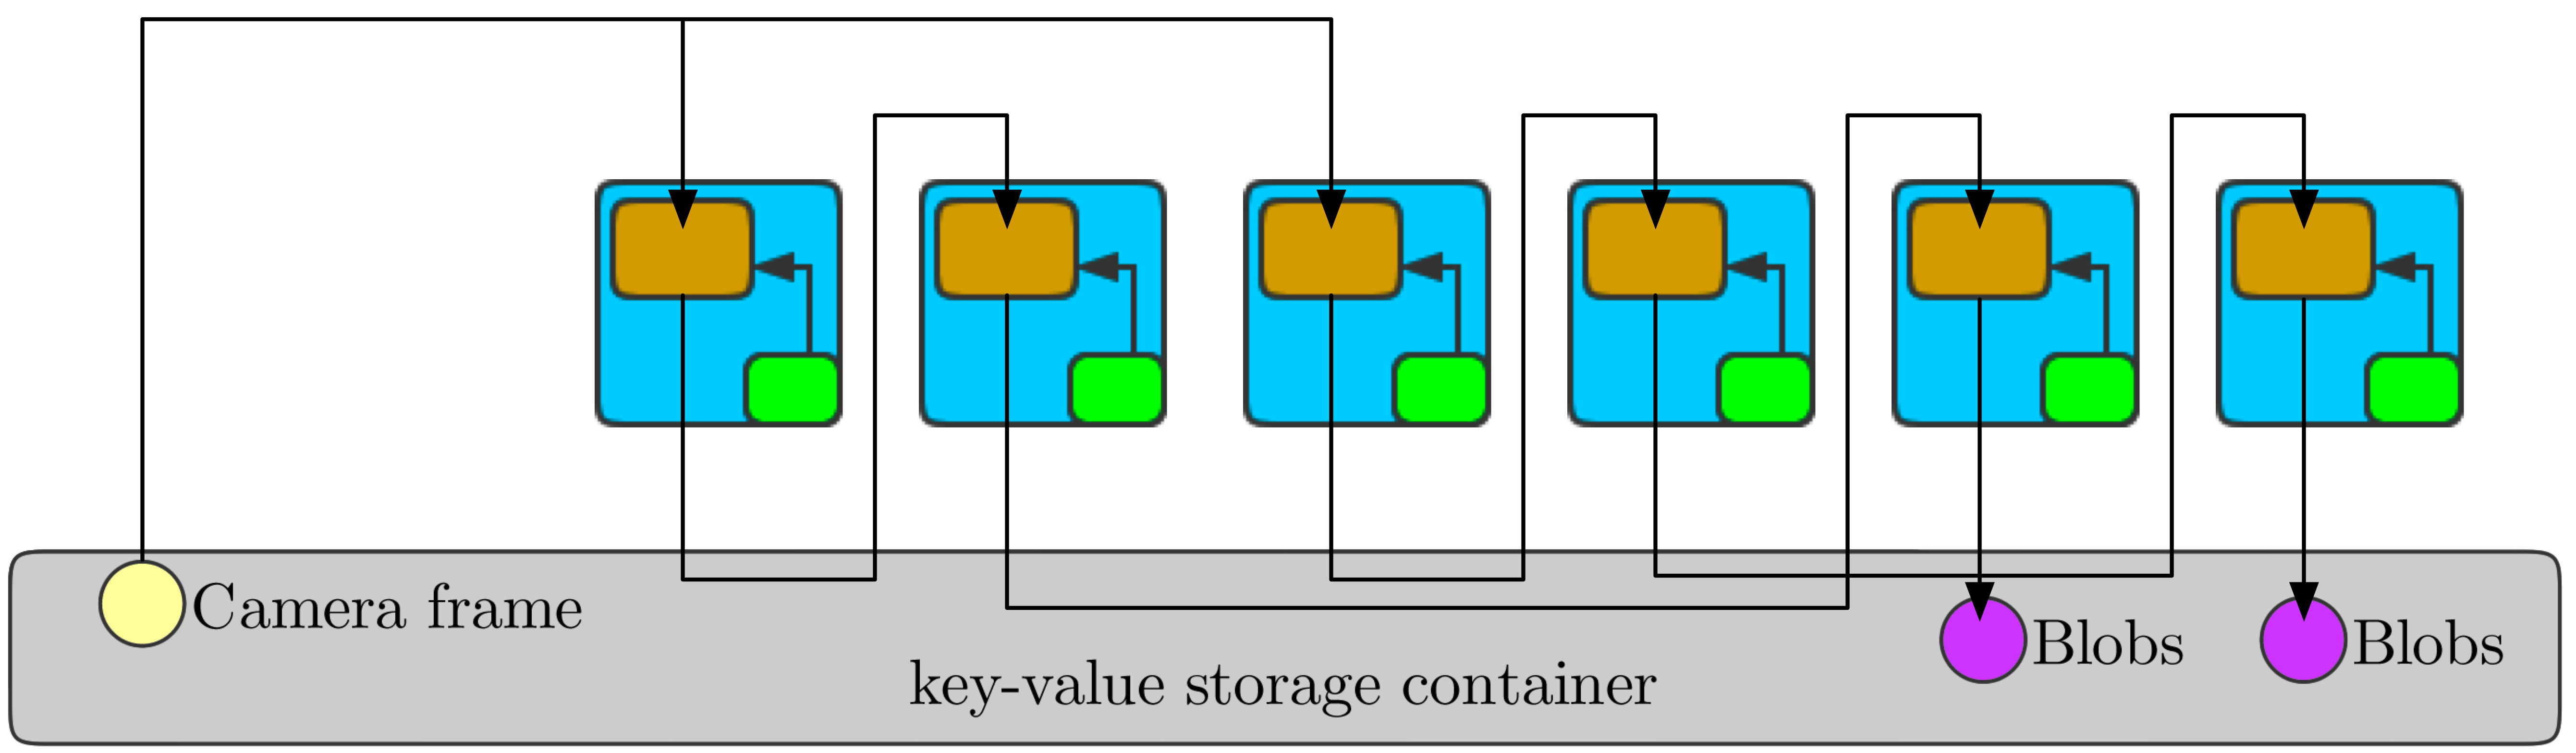
\includegraphics[width=0.8\textwidth]{images/steps_egr} 
\caption{Specific chain used in this project: sequential execution order independent of input/output cross linking. Each output image is automatically stored in the global storage but filters can specify additional storage objects (like a vector of blob coordinates)}
\label{fig:chain-specific}
\end{figure}

The six image processing algorithms could run on an average of 25 frames per second on a Macbook with an Intel Core Duo at 2.5 Ghz, and with a PS3 Eye camera providing 640$\times$480 pixels frames at 60 frames per second. Initially the tracker loop was slightly faster, but had no locking mechanisms on the storage object. Counterintuitively, without locking mechanisms used the CPU up to 90\% with an average of 29 frames per second, but with locking mechanisms the CPU utilization averaged at 45\% and 25 frames per second.
However the locking mechanisms were indispensable: without them random crashes occurred frequently. 

The following table presents the filter chain CPU utilization in milliseconds:

\begin{table}[h]
\caption{Filter processing times}
\tablestyle
\begin{tabular}{*{2}{v{0.3\textwidth}}}
\toprule
   \tablehead Filter &
   \tablehead Processing time \tabularnewline
\midrule
Lab threshold filter (green) & 9.7 ms \tabularnewline
Erosion filter (green) &  1.5 ms \tabularnewline
Blob detection (green) & 6.6 ms \tabularnewline
Lab threshold filter (red) & 9.8 ms \tabularnewline
Erosion filter (red) & 1.2 ms \tabularnewline
Blob detection (red) & 5.5 ms \tabularnewline
Add filter & 1.5 ms \tabularnewline
Add filter & 0.4 ms \tabularnewline
Tracker overhead & 2.1 ms \tabularnewline
\bottomrule
\textbf{Total} & \textbf{38.3 ms} \tabularnewline
\bottomrule
\end{tabular}
\label{tbl:filters-time}
\end{table}

The resulting filtered images of this specific filter chain are presented in chapter \ref{chap:evaluation} (see figure \ref{fig:tracker-chain}).

%%%-%-%-%-%-%-%-%-%-%-%-%%-%-%-%-%-%-%-%-%-%-%-%%%
\section{Model mapping}
\label{sec:model-mapping}

The model mapping is a step in gesture recognition that is not always necessary, depending on the recognition process. But it is helping to accumulate information gathered from the tracker in a structured way, eventually with some transformations applied, in order to exploit physical constraints of the hand. 
In this project, several simple physical constraints are implemented, but the model of the hand could implement more complex constraints, like generalised constraints for the degrees of freedom for the fingers or the distinction of the left and right hand.

%------------------------------------------------%
\subsection{Hand model}
\label{sub:hand-model}

In chapter \ref{chap:chosen-gestures} the interface control gestures of pointing, pinching (zoom) and swiping were chosen. These can be decomposed in the following distinct postures:
\begin{itemize}
\item Pointing posture
\item Pinching posture
\item Posture with all the fingers on the left side (part of the swiping gesture)
\item Posture with all the fingers on the right side (part of the swiping gesture)
\end{itemize}

\begin{figure}[H]
	\centering
	\subfloat[Pointing]{
\includegraphics[width=0.22\textwidth]{images/hand_pointing}}
	\hspace{0.03\textwidth}
	\subfloat[Pinching]{
\includegraphics[width=0.22\textwidth]{images/hand_zooming}}
	\hspace{0.03\textwidth}
	\subfloat[Fingers left]{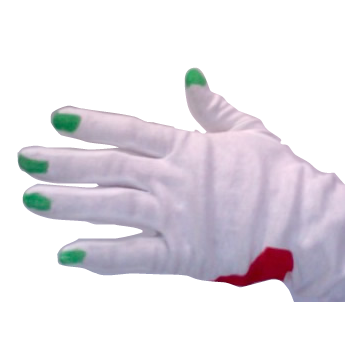
\includegraphics[width=0.22\textwidth]{images/hand_left}}
	\hspace{0.03\textwidth}
	\subfloat[Fingers right]{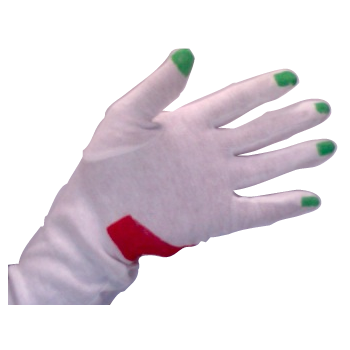
\includegraphics[width=0.22\textwidth]{images/hand_right}}
	\caption{Postures of hand with glove}
	\label{fig:glove-postures}
\end{figure}

The hand model should adhere to the following simple generalisations:

\begin{itemize}
\item A hand has five fingers.
\item A hand has one wrist.
\item Though crossing of fingers is physically possible, it is not very natural and easy to do: there is a circular order of the fingers and the model asserts that it remains (mostly) constant.
\item The index finger and the thumb are the most articulated fingers, while the little finger, the ring finger, and sometimes the middle finger follow the same motion patterns (synchronously): the positions of the little finger and the ring finger can be estimated together.
\end{itemize}

A hand model constructed according to these generalisations should at least contain the following properties:
\begin{itemize}
\item Five finger coordinates
\item Wrist coordinate
\item Order to the fingers: index finger follows the middle finger, thumb follows the index finger
\item Velocity vectors of fingers and wrist
\end{itemize}

%------------------------------------------------%
\subsection{Mapping}
\label{sub:mapping}

To map the unordered vector of finger coordinates and the wrist coordinates obtained from the tracker to the model described in \ref{sub:hand-model}, several mechanisms involving prediction of the coordinates for the next frame, along with an algorithm that finds the best permutation of recognized fingers to the prediction of the previous finger coordinates have been investigated. But the most robust mapping followed the generalization property, that the fingers have a specific order: once the index finger has been identified, the next fingers are mapped according to a circular path along the mass center of all the points (see figure \ref{fig:hand-model}):

\begin{enumerate}
\item Calulate mass center of all points. The wrist has double wheight.
\item Calculate angles $\alpha_{1\ldots n}$ of the vectors from the mass center to each finger coordinate.
\item Sort the fingers according to this angle $\alpha_{1\ldots n}$ in descending order.
\item Cycle the finger vectors in order to position the index finger as the first finger.
\item Missing fingers are calculated as an average of all the fingers without index finger and thumb (first and last finger of the fingers vector).
\end{enumerate}

\begin{figure}[H]
\center
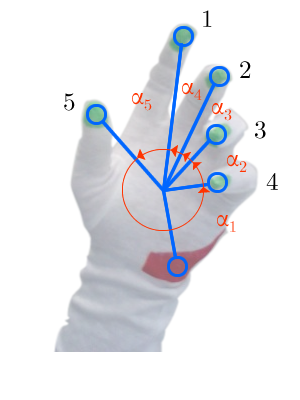
\includegraphics[width=0.275\textwidth]{images/hand-model} 
\caption{Glove with overlayed hand model. $\alpha_{1\ldots n}$ indicates the angle of the vectors from the mass center to each finger coordinate. }
\label{fig:hand-model}
\end{figure}

%%%-%-%-%-%-%-%-%-%-%-%-%%-%-%-%-%-%-%-%-%-%-%-%%%
\section{Training and classification}
\label{sec:training-and-classification}

Initially, attempts were made to directly classify the gesture using a Hidden Markov Model (HMM) as classifier and the set of coordinates of the fingers, or alternatively some other features best describing the gesture in question, as input of this classifier. For this, a test program was implemented, where different features of gesture could be temporally inspected: beside the coordinates, a feature that look promising was the distance of each finger to the wrist or the mass center. This length would also, in a general way, characterize the contraction of the finger, reducing the degree of freedom of each finger in a physical, two-dimensional model to one.

However, it became clear that even if this approach would eventually work, it still was not viable for real-time control gestures. Imagine a scenario where a trained classifier was fed with samples of finger coordinates for each new frame. Two common problems of gesture recognition would arise: when does a gesture begin, and when does it end? But assuming these key moments could somehow be identified, the HMM would still only classify the gesture correctly at its end. At a closer inspection of the gestures defined in section \ref{sec:gestures}, it appeared, that the interface needed to know that the user was pointing somewhere, as soon the he entered a key posture (namely the pointing posture). Equally, as soon the user would stop pointing, the interface does not need to update a cursor position. This led to another approach, which follows more closely the definition of gestures being a sequence of postures.

The recognition approach implemented in this project consists of two parts: 
\begin{enumerate}
\item Posture training and classification from finger coordinates
\item Gesture classification from posture sequences.
\end{enumerate}
This separation allows real-time interaction, as posture classification is frame-based and could have an effect on the interface nearly instantaneously, whereas gestures are time-dependent and require several frames to take effect.

%------------------------------------------------%
\subsection{Sample collection}
\label{sub:sample-collection}

The process of sample collection requires one or more recorded videos containing sequences of postures selected in section \ref{sub:hand-model} and conforming to the constraints of section \ref{sub:environmental-constraints}. Additionally, a way of pre-labeling the postures semi-automatically was put in place, which eliminated the need of manually labeling each posture. This was not strictly necessary, but helped substantially for labeling one minute of video: 60 seconds $\times$ 25 frames per second results in 1500 frames, or approximately 1200 usable postures. The pre-labeling process included a file for the labels, which consisted in a simple text-based subtitle file. This subtitle file had the advantage that it could be edited in any subtitle editor (see figure \ref{fig:subtitle-editor}). The combination of a video and its subtitle file containing the labels of postures makes it also possible to view and inspect the posture-label mapping in any video player capable of displaying subtitles. With this pre-labeling technique the process of sample collection consisted of:

\begin{enumerate}
\item Roughly pre-label postures in a video with a subtitle editor, resulting in a SRT subtitle file,
\item Set the video as the source of the tracker,
\item Map the resulting blobs to a hand model and label it according to the corresponding frame in the subtitle file (see figure \ref{fig:collect-samples}),
\item Save the supervised collection of labeled postures to a posture database file.
\end{enumerate}

\begin{figure}[H]
\center
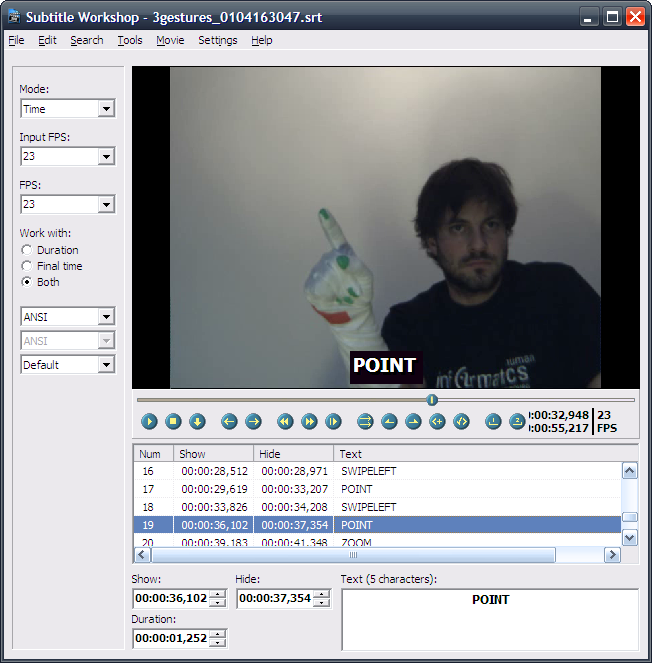
\includegraphics[width=0.67\textwidth]{images/subtitle-editor} 
\caption{Posture labeling with an external subtitle editor. Each posture is labeled with the beginning and the end (in ms) of its presence in the video sequence. This demarcation is the basic structure of a subtitle file. }
\label{fig:subtitle-editor}
\end{figure}

\begin{figure}[H]
\center
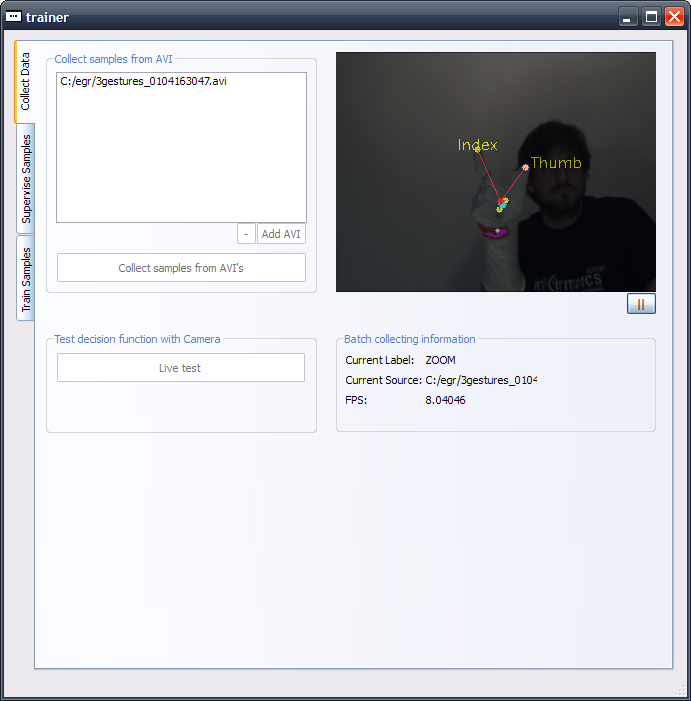
\includegraphics[width=0.67\textwidth]{images/collect-samples} 
\caption{Posture sample collection}
\label{fig:collect-samples}
\end{figure}

%------------------------------------------------%
\subsection{Sample supervision}
\label{sub:sample-supervision}

In a first attempt a support vector machine was trained with the posture samples database obtained from section \ref{fig:collect-samples}. But even the parameter estimation for the support vector machine with a cross validation algorithm did not finish to run in days. At a closer inspection of the collected samples, it became apparent that some samples have been mislabeled, due to the rough boundary of beginning and end of a posture sequence obtained from the subtitle file. Other samples included unusable tracking results from background noise or occluded finger positions. In order to provide a correctly labeled sample database to a classifier, a graphical user interface for quick relabeling and posture inspection was implemented (see figure \ref{fig:sample-supervision}). It allowed to view only samples from one label class, relabel them, or remove the sample altogether from the database, due to inconsistent finger coordinates. In a filtered mode, where only one label class was visible, a cumulative view of all the finger positions in this label class was displayed, helping to inspect the overall finger coordinate distribution of this label class (see figure \ref{fig:cumulative-coordinates}). Each view of a sample displays the finger coordinates relative to the wrist position, giving a easily identifiable representation of a posture.

\begin{figure}[H]
\center
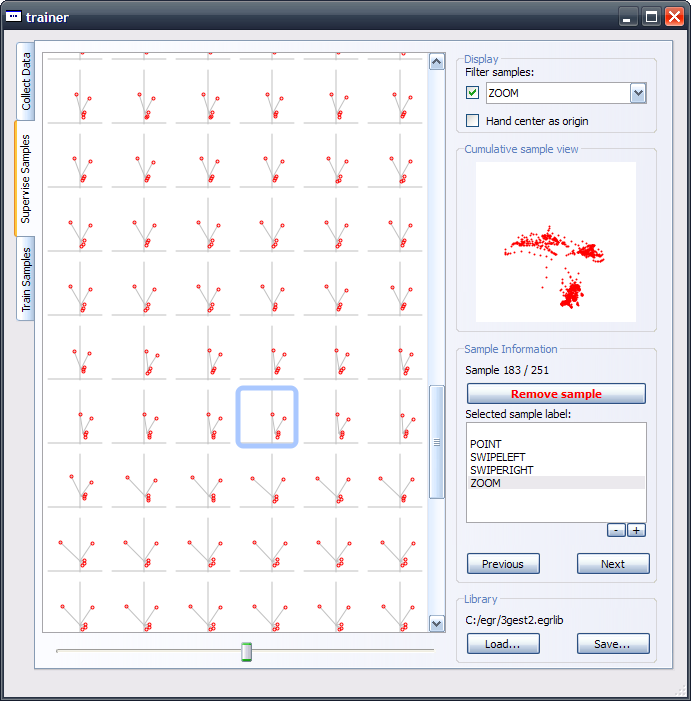
\includegraphics[width=0.67\textwidth]{images/sample-supervision} 
\caption{Sample supervision}
\label{fig:sample-supervision}
\end{figure}

\begin{figure}[H]
	\centering
	\subfloat[Pinching]{
\includegraphics[width=0.18\textwidth]{images/allsamples-zoom}}
	\hspace{0.01\textwidth}
	\subfloat[Pointing]{
\includegraphics[width=0.18\textwidth]{images/allsamples-point}}
	\hspace{0.01\textwidth}
	\subfloat[Fingers on the left]{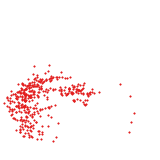
\includegraphics[width=0.18\textwidth]{images/allsamples-left}}
	\hspace{0.01\textwidth}
	\subfloat[Fingers on the right]{
\includegraphics[width=0.18\textwidth]{images/allsamples-right}}
	\hspace{0.01\textwidth}
	\subfloat[Garbage]{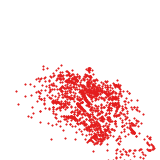
\includegraphics[width=0.18\textwidth]{images/allsamples-empty}}
	\caption{Cumulative view of finger positions for each label}
	\label{fig:cumulative-coordinates}
\end{figure}

%------------------------------------------------%
\subsection{Posture training}
\label{sub:posture-training}

The training of a classifier is done using the dlib C++ library, which packages many classification, regression and clustering algorithms in its machine learning module:
\begin{itemize}
\item Classification (binary): Relevance Vector Machine (RVM), C-Support Vector Machine (C-SVM), C-SVM using empirical kernel maps, linear C-SVM, $\nu$-SVM, Pegasos-SVM
\item Regression: Kernel Recursive Least Squares (KRLS), Kernel Ridge Regression (KRR), Multilayer Perceptron (MLP), $\epsilon$ Support Vector Regression ($\epsilon$-SVR)
\item Kernels: linear kernel, polynomial kernel, radial basis function kernel, sigmoid kernel
\end{itemize}

For this project a multi-class $\nu$-SVM will be used to train a decision function, in order to distinguish between the different classes of postures. A non-linear support vector machine with a kernel function  is ideally suited for this task: a support vector machine separates a set of objects using a linear boundary, or decision plane. However not every classification problem is linearly separable: but the kernel function can rearrange, or transform the objects in a higher-dimensional space, known as feature-space, so that a hyperplane in this higher-dimensional space can linearly separate these objects \cite{svmbook} (see figure \ref{fig:svm-boundary}).

\begin{figure}[H]
	\centering
	\subfloat[Non-linear decision boundary]{\includegraphics[scale=0.5]{images/svm1}}
	\hspace{0.03\textwidth}
	\subfloat[Linear decision boundary in feature space]{\includegraphics[scale=0.5]{images/svm2}}
	\caption{Example of a non-linearly separable classification \cite{svmbook}}
	\label{fig:svm-boundary}
\end{figure}

The feature vector $\textbf{v}$ used to train the $\nu$-SVM is a 10-dimensional vector containing the two-dimensional coordinates of the five fingers:
\[ \textbf{v} = \begin{pmatrix} x_1 \\ y_1 \\ \vdots \\ x_5 \\ y_5  \end{pmatrix} \]

The decision function is trained using a one versus one training structure: since the classifiers provided by dlib are binary classifiers, this structure creates for $n$ possible classes $\frac{n\cdot(n-1)}{2}$ binary classifiers to vote on the identity of a test sample. For the 4 possible postures defined in section \ref{sub:hand-model} there will be 5 classes, including a garbage posture representing everything not belonging to the other 4 postures.

This trained classifier produces a decision function that has an accuracy of 94\% on the training data.

%------------------------------------------------%
\subsection{Posture classification}
\label{sub:posture-classification}

In a cross-validation test the decision function obtained in section \ref{sub:posture-training} produces a confusion matrix, represented in table \ref{tbl:confusion}. This confusion matrix qualitatively gives an indication if the classifier will work on similar test samples. 

\begin{table}[h]
\caption{Confusion matrix of the trained decision function}
\tablestyle
\begin{tabular}{*{6}{v{0.12\textwidth}}}
\toprule
    Identified as: &
    Garbage &
    Pointing &
    Left &
    Right &
    Zoom \tabularnewline
\midrule
\tablehead Garbage & 283 & 11 & 8 & 12 & 3  \tabularnewline
\tablehead Pointing & 14 & 383 & 0 & 0 &0  \tabularnewline
\tablehead Left & 6 & 0 & 71 & 1 & 0 \tabularnewline
\tablehead Right & 8 & 0 & 0 & 166 & 0  \tabularnewline
\tablehead Zoom & 4 & 1 & 0 & 0 & 247  \tabularnewline

\bottomrule
\end{tabular}
\label{tbl:confusion}
\end{table}

In a live test with the camera, the accuracy is subjectively very good for the postures of pinching, with all the fingers on the left and with all the fingers on the right. However there are more misclassifications of the pointing posture, identified as a posture with all the fingers on the right. Going back to section \ref{sub:sample-supervision}, a simple comparison of the cumulative finger positions for each label class does not reveal large overlaying areas for the finger coordinates distribution of these postures (see dark regions in figure \ref{fig:cumulative-comparision}).

\begin{figure}[H]
	\centering
	\subfloat[Left (blue), garbage (orange), right (green)]{\includegraphics[scale=0.55]{images/allsamples-left-nothing-right}}
	\hspace{0.01\textwidth}
	\subfloat[Pointing (red), pinching (green)]{\includegraphics[scale=0.55]{images/allsamples-point-zoom}}
	\hspace{0.01\textwidth}
	\subfloat[Pointing (red), right (green)]{\includegraphics[scale=0.55]{images/allsamples-point-right}}

	\caption{Overlayed cumulative view of finger positions}
	\label{fig:cumulative-comparision}
\end{figure}

But these misclassifications can be filtered out with simple majority filter with a window size that is still acceptable for real-time posture classification. With a window size of 10 frames, which equals 0.4 seconds at 25 FPS, a majority can often be reached in 0.2 seconds, therefore providing a more robust posture classification, that still has a very low reaction time.

%------------------------------------------------%
\subsection{Gesture classification}
\label{sub:gesture-classification}

The recognition of a gesture can be achieved with an Hidden Markov Model (HMM) for each gesture. The state diagram for the pointing gesture (see figure \ref{fig:pointing-states}) has exactly the same structure as the zooming gesture, where there is only one state for the gesture and the only transition allowing to remain in that state is the key posture to this gesture. 

\begin{figure}[H]
	\centering
	\includegraphics[width=0.5\textwidth]{images/states-pointing}
	\caption{State diagram of pointing gesture}
	\label{fig:pointing-states}
\end{figure}

The swiping gesture has a temporal dependency: the only way to reach the final swiping gesture state is to have  right postures follow left postures, or vice versa for a swiping gesture in the opposite direction (see figure \ref{fig:swiping-states}).
\begin{figure}[H]
	\centering
	\includegraphics[width=0.7\textwidth]{images/states-swipe}
	\caption{State diagram of swiping (from left to right) gesture}
	\label{fig:swiping-states}
\end{figure}

These HMM's could be implemented using the HMM Toolkit \cite{htk}. But for the scope of this project and because of the low complexity of the gesture states the recognition was implemented programmatically without HMM's but respecting the transition logic of the gesture state diagrams.

However, gestures with more complex spatial or temporal dependencies would definitively require of the use of an appropriate structure like a HMM. As a simple example, a gesture with more complex spatial dependencies would be a certain hand posture, i.e. the pointing posture, following a specific trajectory, i.e. a circle, that has a symbolic meaning and is not used for the direct control of a cursor following this trajectory. The feature vector for this specific HMM would not only require the posture label, but also the coordinates of the normalized index finger position.

\chapter{Evaluation}
\label{chap:evaluation}

Following chapter \ref{chap:design-and-implementation} which discusses the design and implementation of the gesture recognition architecture, this chapter presents the results obtained with this system. The results of the chosen filter chain (see section \ref{sub:chosen-filter-chain}) can be seen in figure \ref{fig:tracker-chain}. The results of training a classifier for the postures is discussed in section \ref{sec:evaluation-results}. 
\begin{figure}[H]
	\centering
	\subfloat[Lab thresholding filter]{\includegraphics[width=0.23\textwidth]{images/lab_green}}
	\hspace{0.005\textwidth}
	\subfloat[Erosion filter]{\includegraphics[width=0.23\textwidth]{images/erosion_green}}
	\hspace{0.005\textwidth}
	\subfloat[Lab thresholding filter]{\includegraphics[width=0.23\textwidth]{images/lab_red}}
	\hspace{0.005\textwidth}
	\subfloat[Erosion filter]{\includegraphics[width=0.23\textwidth]{images/erosion_red}}
	\hspace{0.005\textwidth}
	\subfloat[Blob detection filter]{\includegraphics[width=0.23\textwidth]{images/blob_green}}
	\hspace{0.005\textwidth}
	\subfloat[Blob detection filter]{\includegraphics[width=0.23\textwidth]{images/blob_red}}
	\hspace{0.005\textwidth}
	\subfloat[Add filter]{\includegraphics[width=0.23\textwidth]{images/add}}
	\hspace{0.005\textwidth}
	\subfloat[Add filter]{\includegraphics[width=0.23\textwidth]{images/overlay}}
	\caption{Resulting steps from tracker with filter chain from section \ref{sub:chosen-filter-chain}}
	\label{fig:tracker-chain}
\end{figure}


\section{Evaluation results}
\label{sec:evaluation-results}

The different modules and programs have been tested qualitatively with a 55 seconds video recorded at 23 frames per second and containing 23 gestures (5 pointing gestures, 6 zooming gestures and 12 swiping gestures). These 55 seconds of video resulted in 1251 postures and after the sample supervision (see section \ref{sub:sample-supervision})  1219 of them were used for the training (see table \ref{tbl:eval}).

\begin{table}[h]
\caption{Postures and gestures of training video}
\tablestyle
\begin{tabular}{*{3}{v{0.2\textwidth}}}
\toprule
   \tablehead gesture name &
   \tablehead number of gestures & 
   \tablehead number of postures \tabularnewline
\midrule
Nothing & 24 & 317\tabularnewline
Pointing & 5 & 397 \tabularnewline
Zooming & 6 & 253 \tabularnewline
Swiping & 12 & 78 (left) \tabularnewline
 &  & 174 (right) \tabularnewline
\bottomrule
\textbf{Total} & \textbf{47} & \textbf{1219} \tabularnewline
\bottomrule
\end{tabular}
\label{tbl:eval}
\end{table}

Once the trainer has a decision function loaded, either by directly training on a sample library or by loading it from a file, it can directly be tested within the trainer using live images from the camera. Analogue to the display of the label from the subtitle during the sample collection (see section \ref{sub:sample-collection}) the label obtained from the decision function is displayed in the same position, indicating the posture that is currently recognized. The filtered posture (see section \ref{sub:posture-classification}) worked remarkably well as long the setup constraints (see section \ref{sub:environmental-constraints}) and the gesture definitions (see section \ref{sec:gestures}) were respected:

\begin{itemize}
\item the distance between glove and camera during the live test should be similar to this distance in the recorded gestures.
\item the lightning conditions are not extreme: the auto-exposure and the auto-gain of the camera have their limits.
\item no background elements should contain green or red colors.
\item tracker can see the characteristic finger blobs of a posture as well as the wrist blob.
\end{itemize}

However, the posture classification is not working well in the following situations:
\begin{itemize}
\item Sometimes when pointing very low, the red marker can not be detected.
\item Pointing to the far right side, without moving the wrist can be classified as a right posture.
\item During the zooming gesture, when thumb and index fingers almost touch each other the classification can result in a posture that is either classified as the pointing posture or the garbage posture.
\end{itemize}

\section{Use case}
\label{sec:use-case}

For the demonstration of an interface controlled by gestures, a small program was implemented (see figure \ref{fig:demo}). This demo program mapped the three gestures from section \ref{sec:gestures} to the following behaviors:

\begin{itemize}
\item Pointing gesture: moves the cursor
\item Zooming gesture: updates a bar indicating the zoom factor
\item Swiping gesture: lets the interface slide in or out on the right side.
\end{itemize}

\begin{figure}[H]
\center
\includegraphics[width=0.7\textwidth]{images/demo} 
\caption{Demo application}
\label{fig:demo}
\end{figure}

This program has no real function other than to demonstrate the recognition of the control gestures. This program was also tested with several other users, who mentioned the following feedback:
\begin{itemize}
\item the reaction time is very fast,
\item the gestures are easy to learn,
\item a real gestural interface would require more gestures, of the same complexity level (i.e. a vertical swipe or grabbing gesture)
\end{itemize}  


\chapter{Conclusion and outlook}
\label{chap:conclusion-and-outlook}

This chapter will recapitulate the master thesis, point out the achievements and mention areas of improvement and problems. \\
In chapter \ref{chap:introduction} a definition of \textit{ergonomic gestures} and the goals of this project have been presented. In an overview, chapter \ref{chap:gesture-recognition} illustrated the different steps involved in gesture recognition, each with some examples from research. It also outlined the general structure and the focus that this project will have on an implementational level. Chapter \ref{chap:setup-and-frameworks} presented the necessary hardware and software, as well as the constraints limiting the scope of this project. With the proposition of the gestures that this project is focusing on (see chapter \ref{chap:chosen-gestures}), all the preliminary informations were present to propose an architecture for real-time gesture recognition. The design and implementation details of this architecture were further discussed in chapter \ref{chap:design-and-implementation}, whereas chapter \ref{chap:evaluation} evaluated this architecture.

This master thesis project achieved its main goal, namely to design and implement a real-time capable gesture recognition system. 
The most important aspects for ergonomic application control gestures that were also obtained in the evaluation study \cite{psychology} (see section \ref{sec:wizard-of-oz-experiment}) were:
\begin{itemize}
\item Fast reaction time
\item Gestures that are easy to learn and can be generalized into an execution of motions and key postures that can be shared among multiple users
\end{itemize}
Additionally to these achievements, the system is also able to recognize small differences and track precisely the small-grained (i.e. zoom factor of the pinching gesture), articulated nature of ergonomic gestures. 

For more complex gestures several future developments can be considered as extensions to this master thesis:
\begin{itemize}
\item train more postures and investigate the SVM parametrization to obtain distinguishable posture classification results,
\item use HMM's to classify gestures with complex temporal or spatial dependencies,
\item replace the tracking module with some other real-time capable hand tracking system that does not need the use of a color-marked glove
\end{itemize}



\bibliography{bib/egr}
\clearpage
\listoffigures
\listoftables

\clearpage
\appendix
\phantomsection
\addcontentsline{toc}{part}{Appendix}
% \input{content/Z-Anhang-01-Herleitungen}

%\chapter*{Danksagung}
\chapter*{Appendix}

The appendix contains the following sections:
\begin{itemize}
\item Installation
\item Train a new posture
\item Create a new tracker filter
\item Write an application with EGRHand
\end{itemize}

\section*{Installation}
All the required files are on the CD-ROM in the Prerequisites directory (except Visual Studio 2008).
\subsection*{Visual Studio}
Install Visual Studio 2008 Professional with standard installation options.

\subsection*{OpenCV 2.0}
\begin{enumerate}
\item Download and install the newest 32-bit binary package for CMake  from \\ \url{http://www.cmake.org}
\item Download OpenCV 2.0 from \\ \url{http://sourceforge.net/projects/opencvlibrary/files/opencv-win/2.0/}
\item During the installation, select to add the OpenCV to the system path
\item Make sure the source is also installed (\textit{src}) 
\item Open CMake
\item Set the source code to \texttt{C:\textbackslash OpenCV2.0} and the build directory to \texttt{C:\textbackslash OpenCV2.0\textbackslash build} \\
\includegraphics[scale=0.75]{images/cmake.png} 
\item Click Configure, use the VS2008 C++ compiler\\
\includegraphics[scale=0.75]{images/cmake_compiler.png} 
\item In the build options make sure OpenMP is selected\\
\includegraphics[scale=0.75]{images/cmake_openmp.png} 
\item Click Configure again, and then Build
\item Under \texttt{C:\textbackslash OpenCV2.0\textbackslash build} open \texttt{OpenCV.sln} 
\item Build the solution in Visual Studio under the Debug target and the Release target
\item In Visual Studio, under Tools $\rightarrow$ Options $\rightarrow$ Projects and Solutions $\rightarrow$ VC++ Directories, add the OpenCV library directories and the OpenCV include directory:\\
\includegraphics[scale=0.75]{images/opencv_vs.png}  \vspace*{1cm}\\
\includegraphics[scale=0.75]{images/opencv_vs_i.png} 
\item Add the following line to the system PATH environment variable: \\ \texttt{C:\textbackslash OpenCV2.0\textbackslash build\textbackslash bin\textbackslash Debug;C:\textbackslash OpenCV2.0\textbackslash build\textbackslash bin\textbackslash Release;} \\(In Computer $\rightarrow$ Properties $\rightarrow$ Advanced $\rightarrow$ Environment Variables)
\end{enumerate}

\subsection*{libconfig}
\begin{enumerate}
\item Download libconfig 1.4.6 from \\ \url{http://www.hyperrealm.com/libconfig/}
\item Extract it to \texttt{C:\textbackslash libconfig-1.4.6}
\item Open \texttt{C:\textbackslash libconfig-1.4.6\textbackslash libconfig.sln} and build the solution under the Debug and Release target.
\item Add the following line to the system PATH environment variable: \\ \texttt{C:\textbackslash libconfig-1.4.6\textbackslash Debug;C:\textbackslash libconfig-1.4.6\textbackslash Release;} \\(In Computer $\rightarrow$ Properties $\rightarrow$ Advanced $\rightarrow$ Environment Variables) 
\end{enumerate}
\subsection*{cvBlobsLib}
\begin{enumerate}
\item Download cvBlobsLib from \\ \url{http://opencv.willowgarage.com/wiki/cvBlobsLib}
\item Extract it to \texttt{C:\textbackslash cvblobslib}
\item Open \texttt{C:\textbackslash cvblobslib\textbackslash cvblobslib.dsp} and convert to a VS 2008 Solution
\item Build the solution under the Debug and Release target
\end{enumerate}
\subsection*{dlib}
\begin{enumerate}
\item Download dlib C++ from \\ \url{http://dlib.net}
\item Extract the entire archive to \texttt{C:\textbackslash dlib-17.34}
\end{enumerate}
\subsection*{PS3 Eye}
\begin{enumerate}
\item Download the CL Eye Platform Driver and the CL Eye Platform SDK from \\ \url{http://codelaboratories.com/downloads}
\item Install the driver and the SDK
\item Add the CL Eye SDK library directory to the system PATH environment variable: \\ \texttt{C:\textbackslash Program Files\textbackslash Code Laboratories\textbackslash CL-Eye Platform SDK\textbackslash Bin;} (In Computer $\rightarrow$ Properties $\rightarrow$ Advanced $\rightarrow$ Environment Variables) 
\end{enumerate}
\subsection*{Qt 4.7.1}
These installation instructions were taken from \\ \url{https://dcsoft.wordpress.com/2010/01/30/}
\begin{enumerate}
\item Download Qt from \\ \url{http://get.qt.nokia.com/qt/source/qt-everywhere-opensource-src-4.7.1.zip}
\item Extract the archive to \texttt{c:\textbackslash qt\textbackslash 4.6.1-vc}
\item Add the environment variable QTDIR: \texttt{QTDIR=c:\textbackslash qt\textbackslash 4.6.1-vc} and the following line to the system PATH environment variable: \texttt{\%QTDIR\%\textbackslash bin} (In Computer $\rightarrow$ Properties $\rightarrow$ Advanced $\rightarrow$ Environment Variables) 
\item Open a Visual Studio Command Prompt and navigate to the \texttt{c:\textbackslash qt\textbackslash 4.6.1-vc} directory
\item Type \texttt{configure -platform win32-msvc2008 } and follow the instructions
\item Type \texttt{nmake} to build Qt.
\item Make sure the following line is added to the system PATH environment variable: \texttt{c:\textbackslash qt\textbackslash 4.6.1-vc\textbackslash bin} (In Computer $\rightarrow$ Properties $\rightarrow$ Advanced $\rightarrow$ Environment Variables) 
\item Download the Visual Studio Qt Addin from \\ \url{http://qt.nokia.com/downloads/visual-studio-add-in}
\item Install the VS Qt Addin
\item In Visual Studio under Qt $\rightarrow$ Qt Options, add the Qt version 4.7.1-vc: \\ \texttt{c:\textbackslash qt\textbackslash 4.6.1-vc}

\end{enumerate}
\subsection*{EGR}
\begin{enumerate}
\item Create the \texttt{c:\textbackslash egr} directory
\item Copy the the files \texttt{tracker.cfg} and \texttt{3gest.egrdf} to this directory
\end{enumerate}
\clearpage

\section*{Train a new posture}
\begin{enumerate}
\item Record a video with \texttt{recorder.exe} (in \texttt{EGR\textbackslash Release})\\
\includegraphics[scale=0.75]{images/recorder} 
\item Edit the posture labels with a subtitle editor (i.e. Subtitle Workshop from \url{http://www.urusoft.net}):
As soon the posture is visible as it is intended to be captured, set the beginning of a new subtitle label. Set the end of the subtitle label when the posture is not anymore in the intended arrangement.
\item Save the posture subtitle file in SubRip (*.srt) format, with the exact same name as the video file.
\item Launch \texttt{trainer.exe} (in \texttt{EGR\textbackslash Release}) \\
\includegraphics[scale=0.75]{images/collect-samples} 
\item Add the Video file and click \textit{Collect Samples from AVI's}
\item When the sample collection is finished, go to the \textit{Supervise samples} tab and save the samples library.\\
\includegraphics[scale=0.75]{images/sample-supervision} 
\item Make sure one label class contains all and only correct postures: 
\begin{itemize}
\item erase postures with coordinates far off the usual area
\item navigate with a click on the posture representation or with \textit{Previous} and \textit{Next}
\item change the label of a posture sample by clicking on the correct label in the list \textit{Selected sample label}
\end{itemize}
\item Save the supervised sample library again and go to the \textit{Train Samples} tab\\
\includegraphics[scale=0.75]{images/train} 
\item Click Train. When the training is finished the progress bar indicates the accuracy in a cross-validation and the text area contains the confusion matrix of the trained decision function
\item Save the decision function
\end{enumerate}
\clearpage

\section*{Create new tracker filter}
\begin{enumerate}
\item Create a new C++ class for \texttt{NewFilter} (\texttt{NewFilter.cpp} and \texttt{NewFilter.h}) in the tracker project.
\item \texttt{NewFilter.h}:\\
\begin{lstlisting}
#pragma once
#include "filter.h"
#include "global.h"

class NewFilter :
	public Filter
{
public:
	NewFilter(void);
	~NewFilter(void);
	NewFilter* clone();
	IplImage* filter(std::vector<IplImage* > images);
}
\end{lstlisting}
\item \texttt{NewFilter.cpp}:\\
\begin{lstlisting}
#include "stdafx.h"
#include "NewFilter.h"

NewFilter::NewFilter(void)
{
	name = "New Filter"; //this name is displayed in the overlay
	sourceCount=1; //number of input images to the filter
    params.push_back(new Parameter(0.0f, 1.0f, 5.0f)); //specify range (minimum, lower bound, upper bound, maximum) with 4 float parameters
}

NewFilter::~NewFilter(void)
{
}

NewFilter* NewFilter::clone(){
	NewFilter *nf = new NewFilter();
    nf->params.clear();
    for(int i=0;i<(int)params.size();i++)
        nf->params.push_back(new Parameter(this->params[i]));
    return nf;
}

IplImage* NewFilter::filter(std::vector<IplImage*> images){
	IplImage *img = 0;
	if(images.size()>0)
		img = images[0];

	Parameter *p = params[0];
	float value = p->getVal();
	if(p != 0 ){
		//do something
	}
	return img;

}
\end{lstlisting}
\item Add the Filter to the \texttt{initFilters()} method in \texttt{main.cpp}. Make sure the name of the filter and the filter object have the same index in the \texttt{strFilterList} and the \texttt{filterList} vectors!
\begin{lstlisting}
void initFilters(){
	strFilterList.push_back("New Filter");
	strFilterList.push_back("Empty Filter");
	strFilterList.push_back("Lab Threshold Filter");
	strFilterList.push_back("Erosion Filter");
	strFilterList.push_back("Dilation Filter");
	strFilterList.push_back("Blob Filter");
	strFilterList.push_back("Add Filter");
	strFilterList.push_back("Threshold Filter");
	strFilterList.push_back("RGB Threshold Filter");
	strFilterList.push_back("Split Filter");
	strFilterList.push_back("Fast Corner Filter");
	strFilterList.push_back("Smooth Filter");
		
	filterList.push_back(new NewFilter());
	filterList.push_back(new EmptyFilter());
	filterList.push_back(new LabThresholdFilter());
	filterList.push_back(new ErosionFilter());
	filterList.push_back(new DilationFilter());
	filterList.push_back(new BlobFilter());
	filterList.push_back(new AddFilter());
	filterList.push_back(new ThresholdFilter());
	filterList.push_back(new RGBThresholdFilter());
	filterList.push_back(new SplitFilter());
	filterList.push_back(new FastCornerFilter());
	filterList.push_back(new SmoothFilter());
	
	
}
\end{lstlisting}
\item Include the new filter header file in \texttt{tracker.h}
\begin{lstlisting}
...
#include "NewFilter.h"
#include "EmptyFilter.h"
...
\end{lstlisting}
\end{enumerate}
\clearpage

\section*{Write application with EGRHand}
\begin{enumerate}
\item In Visual Studio, create a new Project within the EGR solution
\item Under Project Properties $\rightarrow$ Configuration Properties $\rightarrow$ C/C++ $\rightarrow$ General, add the following Include directories:
\begin{itemize}
\item \verb+$(SolutionDir)\model+
\item \verb+$(SolutionDir)\trainer+
\item \verb+c:\dlib-17.34+
\end{itemize}
\item Under Project Properties $\rightarrow$ Configuration Properties $\rightarrow$ Linker $\rightarrow$ General, add the following Library directory: 
\verb+$(OutDir)+
\item Under Project Properties $\rightarrow$ Configuration Properties $\rightarrow$ Linker $\rightarrow$ Input, add the following library dependecies: 
\begin{lstlisting}
model.lib
cv200.lib
highgui200.lib
cvaux200.lib
cxcore200.lib
cxts200.lib
ml200.lib
opencv_ffmpeg200.lib
\end{lstlisting}
\item Include the following header files:
\begin{lstlisting}
#include "EGRHand.h"
#include "egr_dlib.h"
#include "dlib/svm.h"
#include <iostream>
\end{lstlisting}
\item The EGRHand object is initialized as follows:
\begin{lstlisting}
EGRHand *hand = createEGRHand();
//blobs_5: the finger blobs are detected in step 5
//blobs_6: the wrist blob is detected in step 6
hand->init("c:\\egr\\tracker.cfg", "blobs_5", "blobs_6");
//load the decision function 
ifstream fin("c:\\egr\\3gest.egrdf", ios::binary);
deserialize(df, fin);
hand->setClassifier(df);
hand->start();
\end{lstlisting}
\clearpage
\item Retreive information from the EGRHand object as follows:
\begin{lstlisting}
IplImage *tracker_frame = (IplImage *) hand->getTrackerImage("Screen 8");
string posture = hand->getClassifiedPosture();
\end{lstlisting}
\item Take a look at the methods \texttt{handleGesture(string)} and \texttt{filterPostures(string, int)} in the mouse project of the EGR solution.
\end{enumerate}

\IfDefined{printindex}{\printindex}
\IfDefined{printnomenclature}{\printnomenclature}

\end{document}